\documentclass[11pt]{article}
\usepackage[margin=2cm]{geometry}
\usepackage{amsmath,amssymb}
\usepackage{graphicx}
\usepackage{booktabs}
\usepackage{array}
\usepackage{xcolor}
\usepackage[breakable]{tcolorbox}
\usepackage{enumitem}
\usepackage[hidelinks]{hyperref}
\allowdisplaybreaks
\setlength{\parindent}{0pt}
\setlength{\parskip}{4pt}
\definecolor{stepc}{HTML}{1F4E9E}
\definecolor{ansc}{HTML}{0B6E4F}
\newcommand{\solstep}[2]{\par\medskip{\color{stepc}\textbf{Step #1 --- #2}}\par\nopagebreak}
\newtcolorbox{probbox}[1]{colback=white,colframe=black!55,fonttitle=\bfseries,title={#1}}
\newtcolorbox{ansbox}{breakable,colback=ansc!6,colframe=ansc,fonttitle=\bfseries,title={Answer}}
\newtcolorbox{cardbox}[1]{breakable,colback=stepc!4,colframe=stepc,fonttitle=\bfseries,title={#1}}
\graphicspath{{../../../output/lecture4/4D_small_signal/}}
\title{Set 4D: BJT Amplifiers --- Small-Signal Analysis}
\author{ECEN 325 --- Lecture 4 (Bipolar Junction Transistors) practice set}
\date{}
\begin{document}
\maketitle

\textbf{What this set trains.} The small-signal transfer function of single- and multi-stage BJT amplifiers with the
node-impedance method: $r_e$ of every transistor, the input resistance of every stage (from the last one
backwards), and the product of the node-to-node gains along the signal path. Then the Bode plot and the
steady-state output. $\beta = 100$, $V_T = 25$\,mV, $r_o = \infty$; capacitors marked $\infty$ are shorts at the signal
frequencies. The DC collector currents are given (they follow from a DC analysis as in sets 4A/4B). Problems 1--6
are easy, 7--12 medium, 13--18 hard. Try each problem before looking at its solution.


\begin{cardbox}{The Lecture-4 pipeline (use it for every problem in this lecture)}
\textbf{Tools --- this is all the theory you need (plus the Lecture-1--3 tools):}
\begin{enumerate}[label=\textbf{T\arabic*},leftmargin=2.2em,itemsep=1pt]
\item \emph{Active BJT at DC:} npn $V_{BE}=0.7$\,V, pnp $V_{EB}=0.7$\,V; $I_C=\beta I_B$, $I_E=(\beta+1)I_B$, so
      $I_C\approx I_E$ and, when $\beta$ is large, $I_B\approx 0$. Active needs $|V_{CE}|\ge 0.2$\,V.
\item \emph{Current mirror:} transistors with the same base node and the same emitter node have the same $V_{BE}$,
      hence the same $I_C$.
\item \emph{Small-signal parameters:} $r_e = \frac{V_T}{I_C}$ ($V_T=25$\,mV), $\alpha=\frac{\beta}{\beta+1}$, $r_o=\infty$.
      For AC, DC supplies are ground and ``$\infty$'' capacitors are shorts.
\item \emph{Node impedances and gains:} $Z_{base}=(\beta+1)(r_e+Z_E)$, $Z_{emitter}=r_e+\frac{Z_B}{\beta+1}$,
      $Z_{collector}=\infty$;\ \ CE $\frac{v_c}{v_b}=-\alpha\frac{Z_C}{r_e+Z_E}$, CB $\frac{v_c}{v_e}=\alpha\frac{Z_C}{Z_{emitter}}$,
      CC $\frac{v_e}{v_b}=\frac{Z_E}{r_e+Z_E}$. $Z_C$, $Z_E$, $Z_B$ are everything else hanging on that node
      (including the input resistance of the next stage).
\end{enumerate}
\textbf{Steps:}
\begin{enumerate}[leftmargin=2.2em,itemsep=1pt]
\item \emph{DC:} assume every transistor active and $I_B\approx0$; walk through the circuit node by node
      (dividers, $V_{BE}$, KCL for $I_E$, $I_C\approx I_E$, collector voltages); then \emph{verify}: $I_B\ll$ bias currents and
      $|V_{CE}|\ge0.2$\,V.
\item \emph{AC:} $r_e$ of every transistor; input resistance of every stage from the last one backwards; multiply the
      node-to-node gains along the signal path; then standard form, Bode plot and output as in Lecture 1.
\item \emph{Design:} run the same relations backwards, choosing the free quantities with the stated design rules, then
      check the result by analysing the finished circuit.
\end{enumerate}
\end{cardbox}

\section*{Problems}
\subsection*{Easy problems}
\begin{probbox}{Problem 4D.1 \hfill Easy}
For the amplifier below, find the small-signal transfer function $H(s)=\dfrac{V_o(s)}{V_i(s)}$ and sketch its magnitude Bode plot. Also find the steady-state output $V_o(t)$ for $V_i(t) = 0.005\sin\left(2\pi\cdot 1000\,t\right)$. $\beta = 100$, $V_T = 25$\,mV; the DC collector currents are $I_{C1} = 1\,\mathrm{m}\mathrm{A}$.
\begin{center}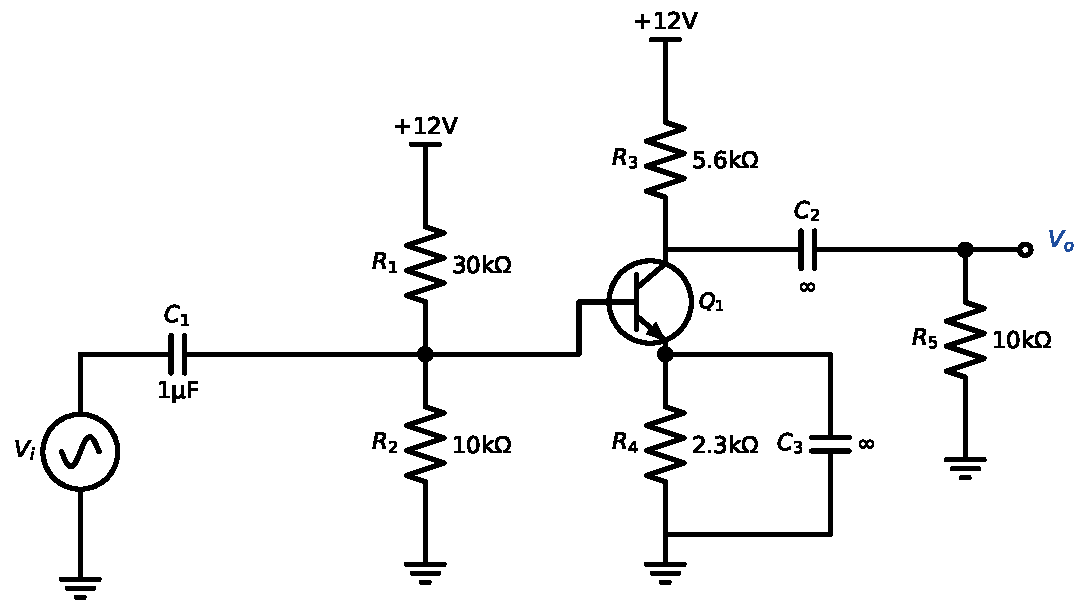
\includegraphics[width=\linewidth,height=7cm,keepaspectratio]{p01_circuit}\end{center}
\end{probbox}

\begin{probbox}{Problem 4D.2 \hfill Easy}
For the amplifier below, find the small-signal transfer function $H(s)=\dfrac{V_o(s)}{V_i(s)}$ and sketch its magnitude Bode plot. Also find the steady-state output $V_o(t)$ for $V_i(t) = 0.05\sin\left(2\pi\cdot 2000\,t\right)$. $\beta = 100$, $V_T = 25$\,mV; the DC collector currents are $I_{C1} = 1\,\mathrm{m}\mathrm{A}$.
\begin{center}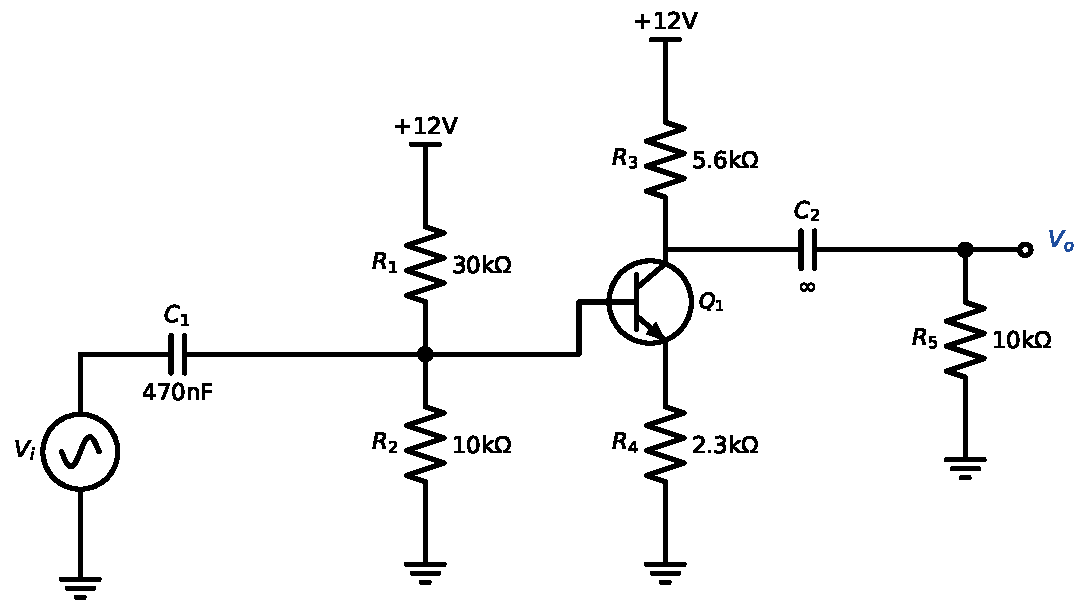
\includegraphics[width=\linewidth,height=7cm,keepaspectratio]{p02_circuit}\end{center}
\end{probbox}

\begin{probbox}{Problem 4D.3 \hfill Easy}
For the amplifier below, find the small-signal transfer function $H(s)=\dfrac{V_o(s)}{V_i(s)}$ and sketch its magnitude Bode plot. Also find the steady-state output $V_o(t)$ for $V_i(t) = 0.5\sin\left(2\pi\cdot 1000\,t\right)$. $\beta = 100$, $V_T = 25$\,mV; the DC collector currents are $I_{C1} = 2\,\mathrm{m}\mathrm{A}$.
\begin{center}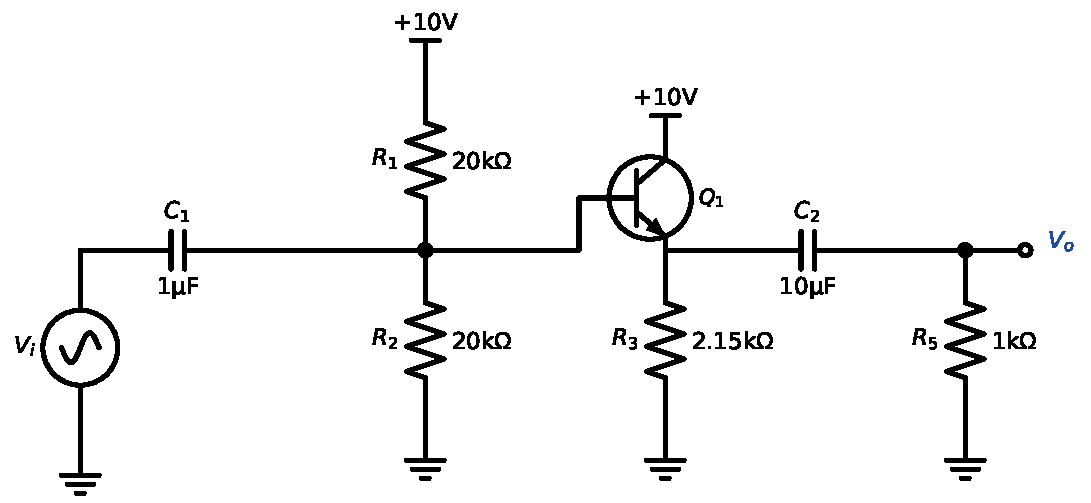
\includegraphics[width=\linewidth,height=7cm,keepaspectratio]{p03_circuit}\end{center}
\end{probbox}

\begin{probbox}{Problem 4D.4 \hfill Easy}
For the amplifier below, find the small-signal transfer function $H(s)=\dfrac{V_o(s)}{V_i(s)}$ and sketch its magnitude Bode plot. Also find the steady-state output $V_o(t)$ for $V_i(t) = 0.01\sin\left(2\pi\cdot 1000\,t\right)$. $\beta = 100$, $V_T = 25$\,mV; the DC collector currents are $I_{C1} = 1\,\mathrm{m}\mathrm{A}$.
\begin{center}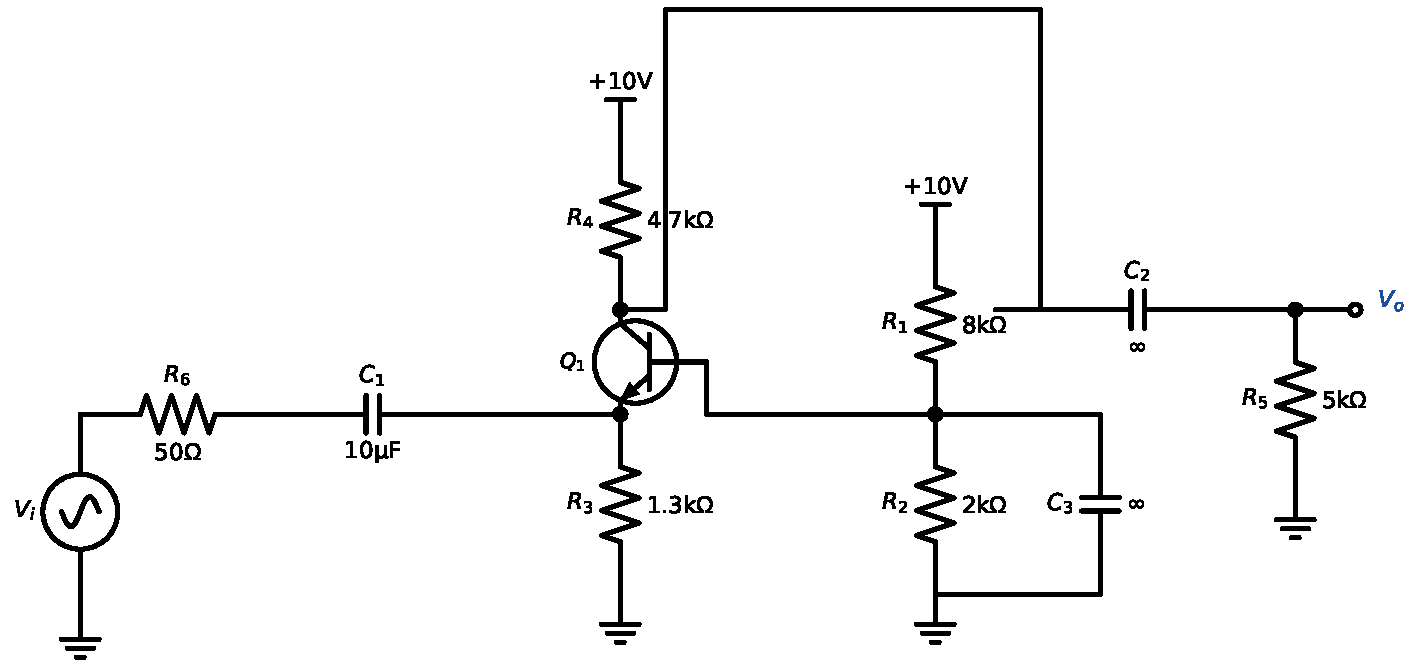
\includegraphics[width=\linewidth,height=7cm,keepaspectratio]{p04_circuit}\end{center}
\end{probbox}

\begin{probbox}{Problem 4D.5 \hfill Easy}
For the amplifier below, find the small-signal transfer function $H(s)=\dfrac{V_o(s)}{V_i(s)}$ and sketch its magnitude Bode plot. Also find the steady-state output $V_o(t)$ for $V_i(t) = 0.002\sin\left(2\pi\cdot 5000\,t\right)$. $\beta = 100$, $V_T = 25$\,mV; the DC collector currents are $I_{C1} = 1\,\mathrm{m}\mathrm{A}$.
\begin{center}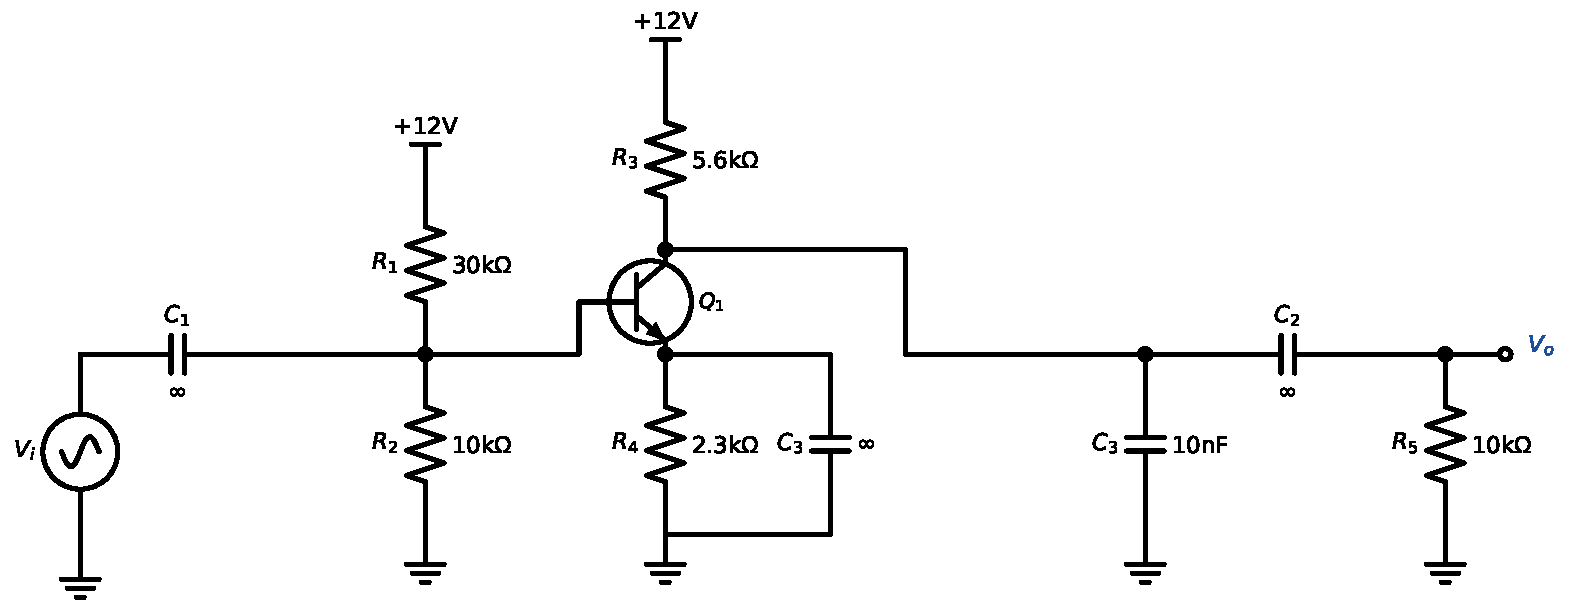
\includegraphics[width=\linewidth,height=7cm,keepaspectratio]{p05_circuit}\end{center}
\end{probbox}

\begin{probbox}{Problem 4D.6 \hfill Easy}
For the amplifier below, find the small-signal transfer function $H(s)=\dfrac{V_o(s)}{V_i(s)}$ and sketch its magnitude Bode plot. Also find the steady-state output $V_o(t)$ for $V_i(t) = 0.005\sin\left(2\pi\cdot 300\,t\right)$. $\beta = 100$, $V_T = 25$\,mV; the DC collector currents are $I_{C1} = 1\,\mathrm{m}\mathrm{A}$.
\begin{center}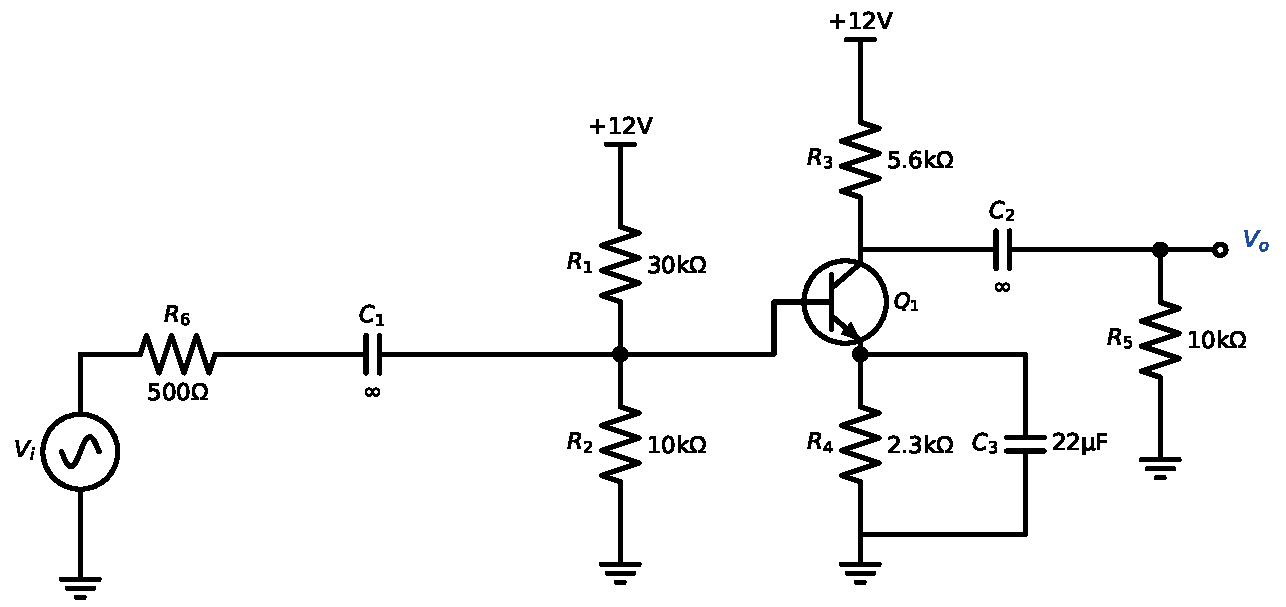
\includegraphics[width=\linewidth,height=7cm,keepaspectratio]{p06_circuit}\end{center}
\end{probbox}

\subsection*{Medium problems}
\begin{probbox}{Problem 4D.7 \hfill Medium}
For the amplifier below, find the small-signal transfer function $H(s)=\dfrac{V_o(s)}{V_i(s)}$ and sketch its magnitude Bode plot. Also find the steady-state output $V_o(t)$ for $V_i(t) = 0.01\sin\left(2\pi\cdot 2000\,t\right)$. $\beta = 100$, $V_T = 25$\,mV; the DC collector currents are $I_{C1} = 1\,\mathrm{m}\mathrm{A}$.
\begin{center}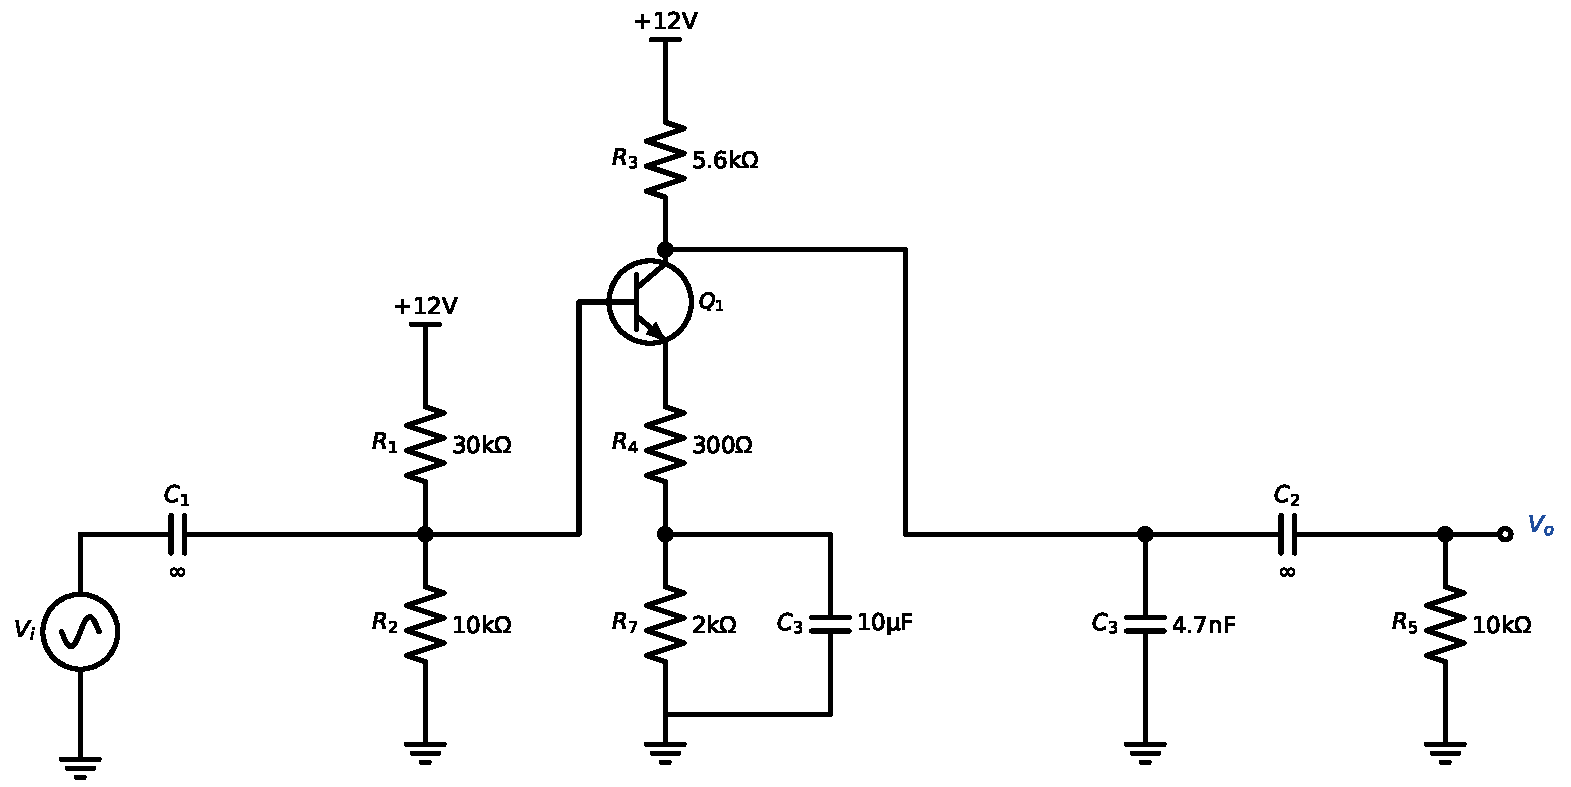
\includegraphics[width=\linewidth,height=7cm,keepaspectratio]{p07_circuit}\end{center}
\end{probbox}

\begin{probbox}{Problem 4D.8 \hfill Medium}
For the amplifier below, find the small-signal transfer function $H(s)=\dfrac{V_o(s)}{V_i(s)}$ and sketch its magnitude Bode plot. Also find the steady-state output $V_o(t)$ for $V_i(t) = 0.002\sin\left(2\pi\cdot 1000\,t\right)$. $\beta = 100$, $V_T = 25$\,mV; the DC collector currents are $I_{C1} = 1.41\,\mathrm{m}\mathrm{A}$, $I_{C2} = 2.13\,\mathrm{m}\mathrm{A}$.
\begin{center}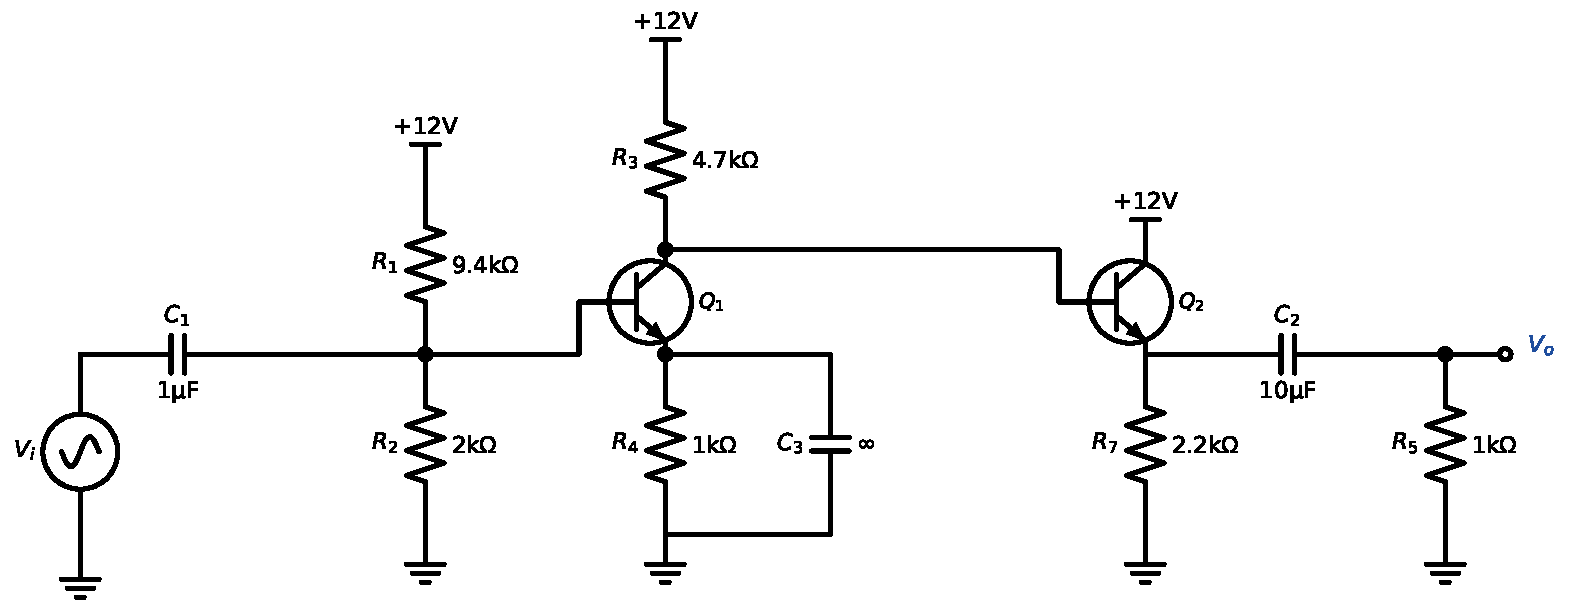
\includegraphics[width=\linewidth,height=7cm,keepaspectratio]{p08_circuit}\end{center}
\end{probbox}

\begin{probbox}{Problem 4D.9 \hfill Medium}
For the amplifier below, find the small-signal transfer function $H(s)=\dfrac{V_o(s)}{V_i(s)}$ and sketch its magnitude Bode plot. Also find the steady-state output $V_o(t)$ for $V_i(t) = 0.005\sin\left(2\pi\cdot 500\,t\right)$. $\beta = 100$, $V_T = 25$\,mV; the DC collector currents are $I_{C1} = 1\,\mathrm{m}\mathrm{A}$, $I_{C2} = 1.73\,\mathrm{m}\mathrm{A}$.
\begin{center}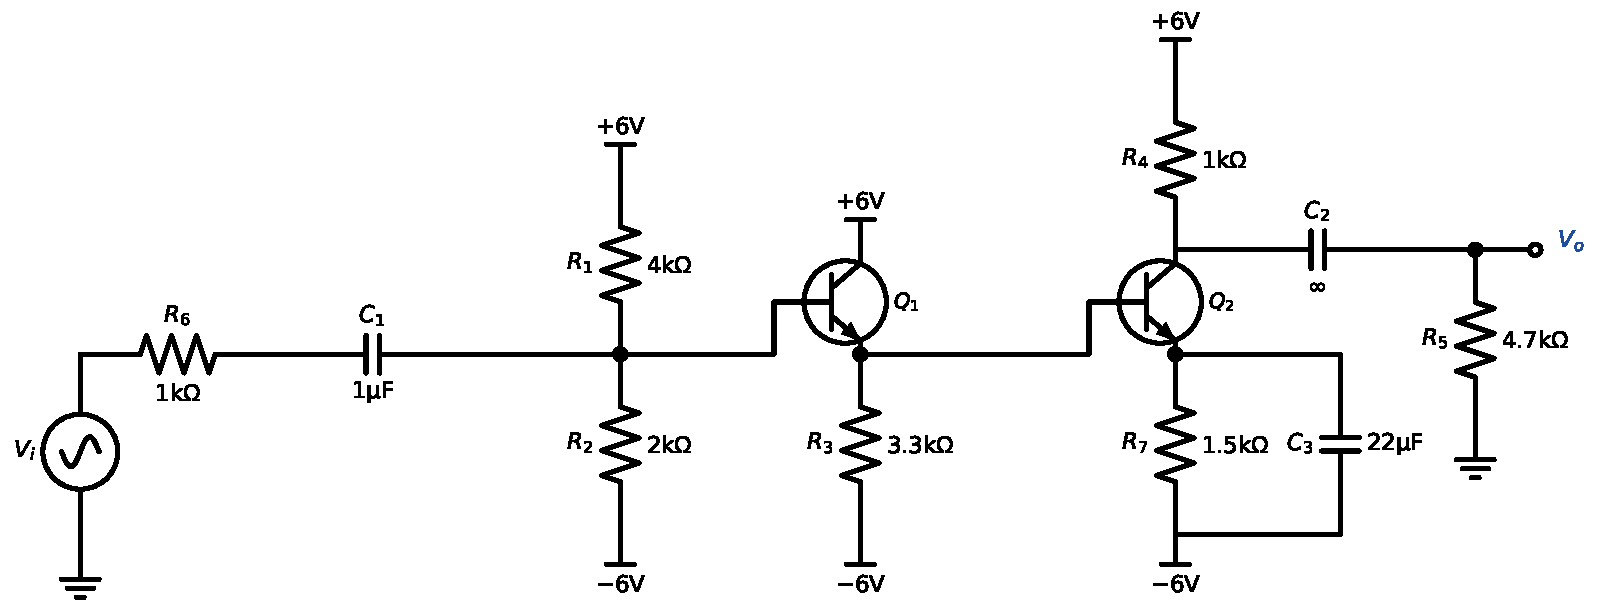
\includegraphics[width=\linewidth,height=7cm,keepaspectratio]{p09_circuit}\end{center}
\end{probbox}

\begin{probbox}{Problem 4D.10 \hfill Medium}
For the amplifier below, find the small-signal transfer function $H(s)=\dfrac{V_o(s)}{V_i(s)}$ and sketch its magnitude Bode plot. Also find the steady-state output $V_o(t)$ for $V_i(t) = 5\times 10^{-4}\sin\left(2\pi\cdot 1000\,t\right)$. $\beta = 100$, $V_T = 25$\,mV; the DC collector currents are $I_{C1} = 1\,\mathrm{m}\mathrm{A}$, $I_{C2} = 1\,\mathrm{m}\mathrm{A}$.
\begin{center}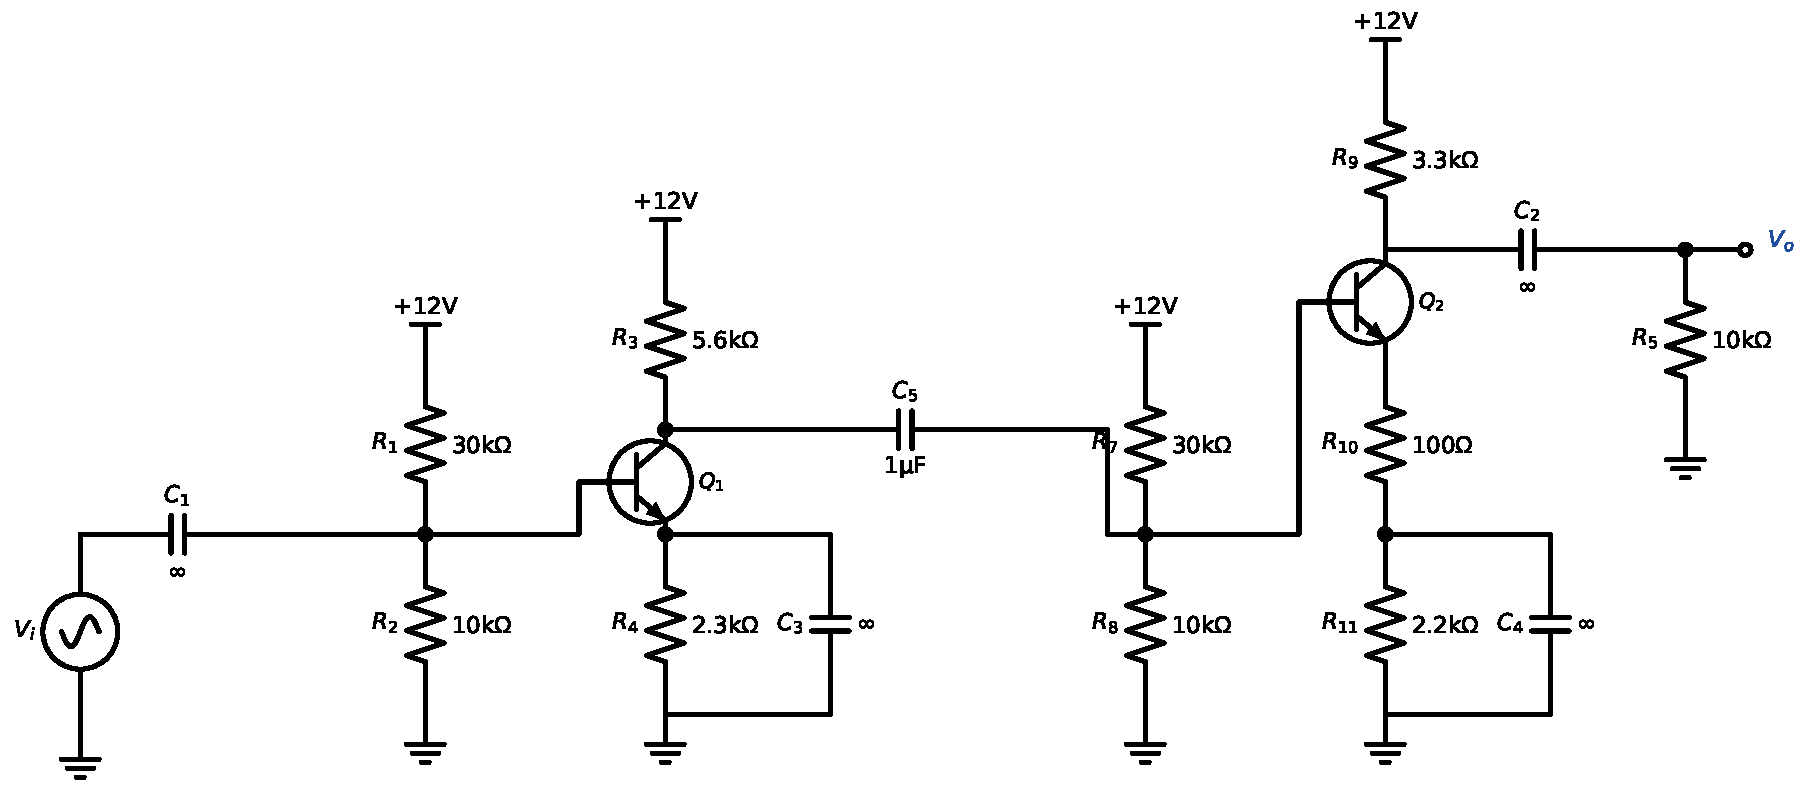
\includegraphics[width=\linewidth,height=7cm,keepaspectratio]{p10_circuit}\end{center}
\end{probbox}

\begin{probbox}{Problem 4D.11 \hfill Medium}
For the amplifier below, find the small-signal transfer function $H(s)=\dfrac{V_o(s)}{V_i(s)}$ and sketch its magnitude Bode plot. Also find the steady-state output $V_o(t)$ for $V_i(t) = 0.02\sin\left(2\pi\cdot 200\,t\right)$. $\beta = 100$, $V_T = 25$\,mV; the DC collector currents are $I_{C1} = 1\,\mathrm{m}\mathrm{A}$.
\begin{center}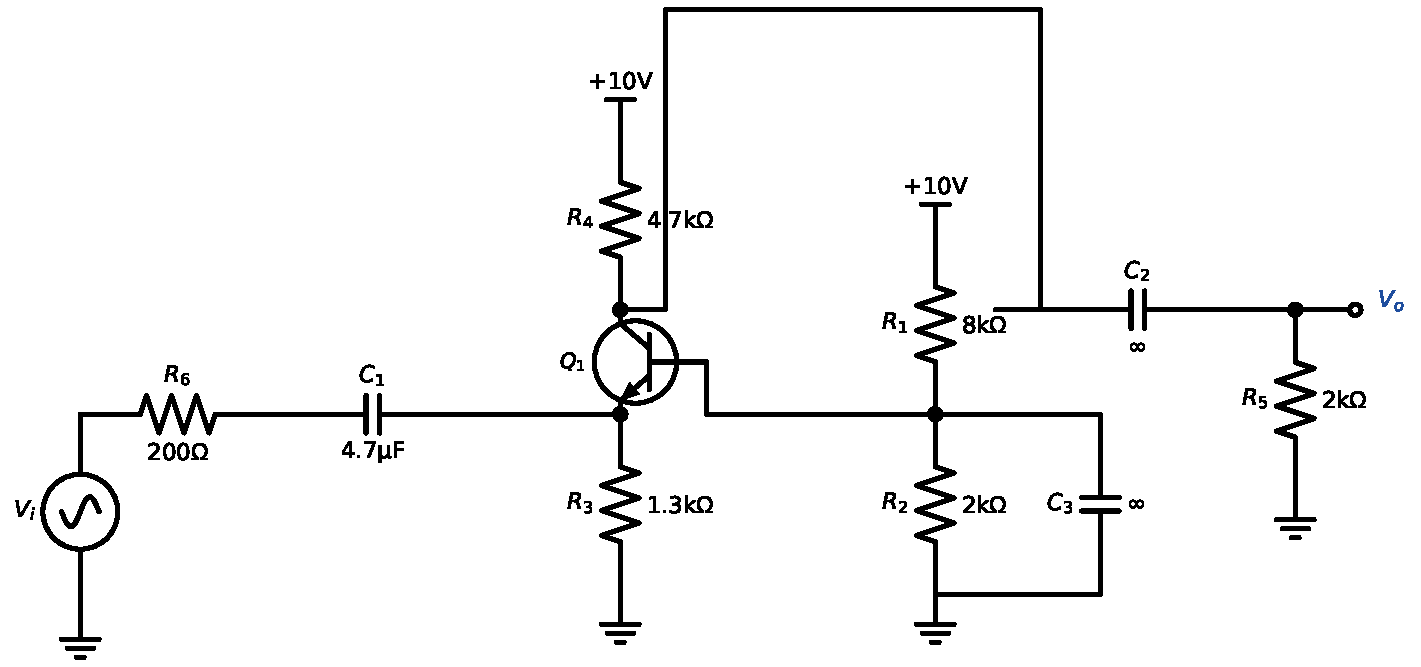
\includegraphics[width=\linewidth,height=7cm,keepaspectratio]{p11_circuit}\end{center}
\end{probbox}

\begin{probbox}{Problem 4D.12 \hfill Medium}
For the amplifier below, find the small-signal transfer function $H(s)=\dfrac{V_o(s)}{V_i(s)}$ and sketch its magnitude Bode plot. Also find the steady-state output $V_o(t)$ for $V_i(t) = 0.02\sin\left(2\pi\cdot 10000\,t\right)$. $\beta = 100$, $V_T = 25$\,mV; the DC collector currents are $I_{C1} = 800\,\mu \mathrm{A}$, $I_{C2} = 800\,\mu \mathrm{A}$, $I_{C3} = 3.1\,\mathrm{m}\mathrm{A}$.
\begin{center}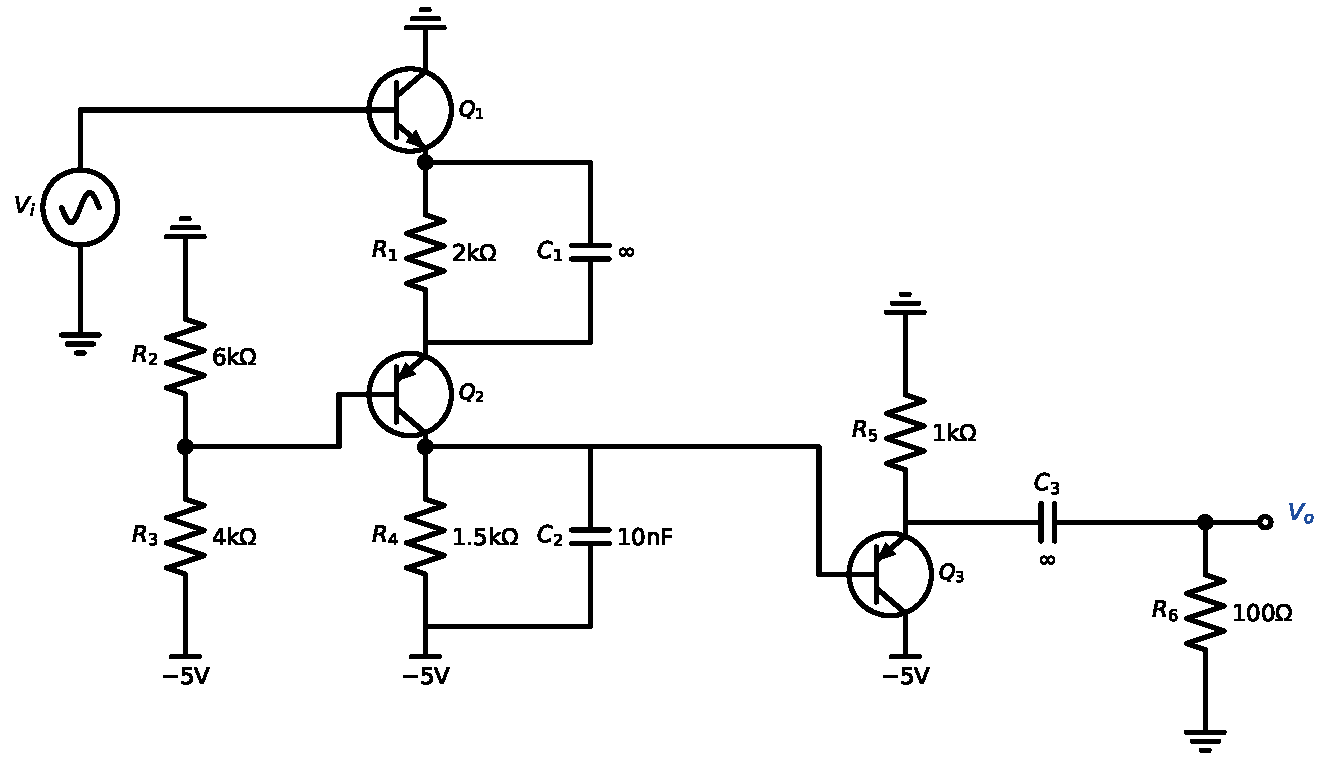
\includegraphics[width=\linewidth,height=7cm,keepaspectratio]{p12_circuit}\end{center}
\end{probbox}

\subsection*{Hard problems}
\begin{probbox}{Problem 4D.13 \hfill Hard}
For the amplifier below, find the small-signal transfer function $H(s)=\dfrac{V_o(s)}{V_i(s)}$ and sketch its magnitude Bode plot. Also find the steady-state output $V_o(t)$ for $V_i(t) = 0.005\sin\left(2\pi\cdot 2000\,t\right)$. $\beta = 100$, $V_T = 25$\,mV; the DC collector currents are $I_{C1} = 900\,\mu \mathrm{A}$, $I_{C2} = 2.4\,\mathrm{m}\mathrm{A}$.
\begin{center}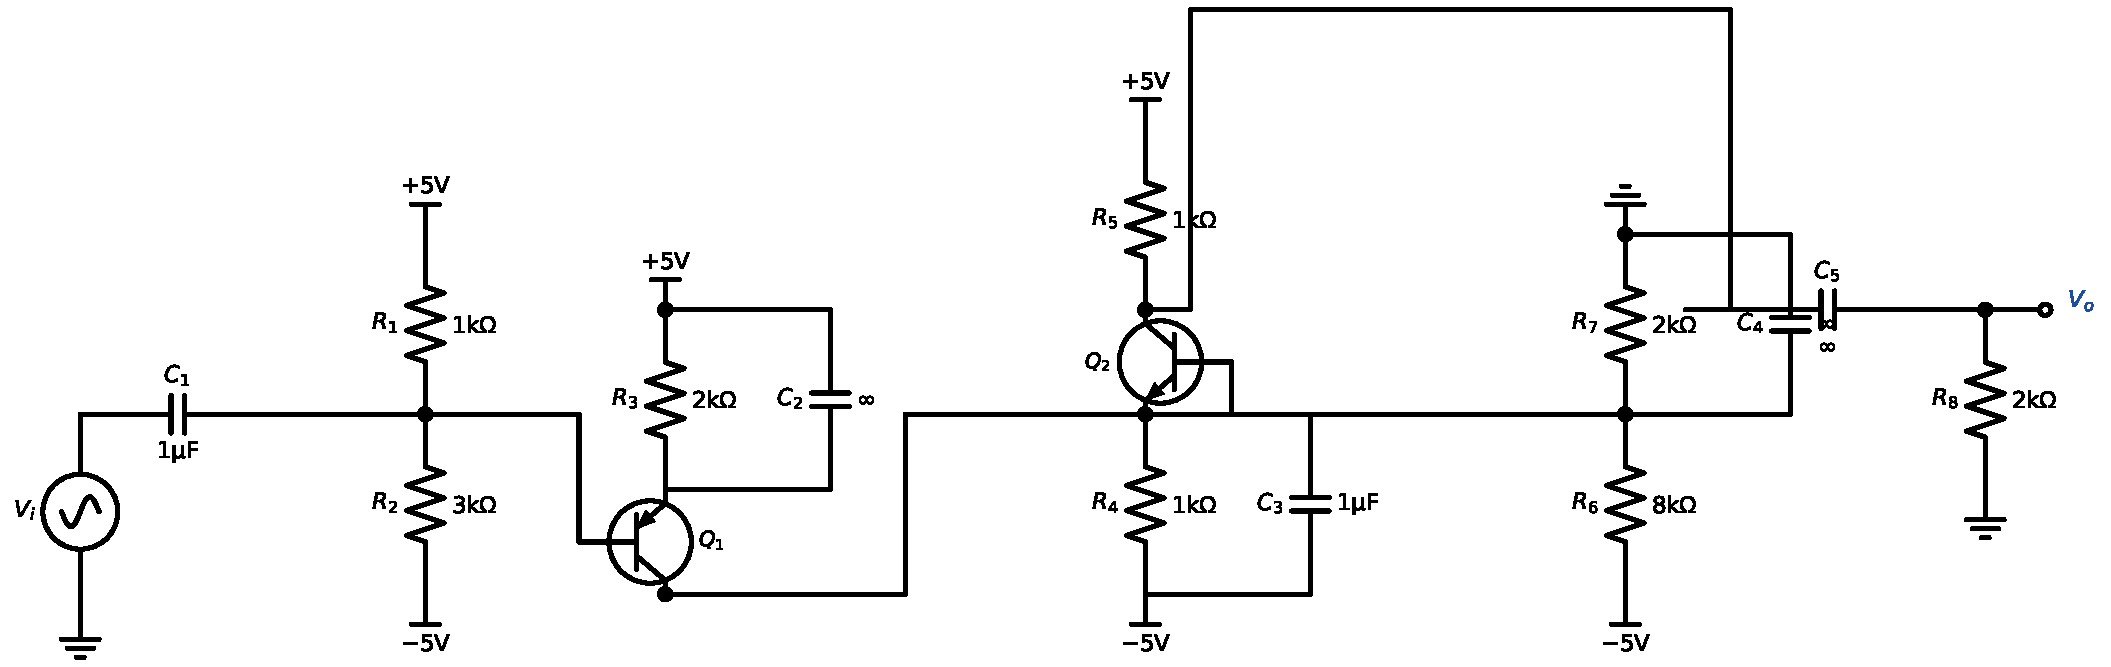
\includegraphics[width=\linewidth,height=7cm,keepaspectratio]{p13_circuit}\end{center}
\end{probbox}

\begin{probbox}{Problem 4D.14 \hfill Hard}
For the amplifier below, find the small-signal transfer function $H(s)=\dfrac{V_o(s)}{V_i(s)}$ and sketch its magnitude Bode plot. Also find the steady-state output $V_o(t)$ for $V_i(t) = 0.05\sin\left(2\pi\cdot 20000\,t+\frac{\pi}{4}\right)$. $\beta = 100$, $V_T = 25$\,mV; the DC collector currents are $I_{C1} = 800\,\mu \mathrm{A}$, $I_{C2} = 800\,\mu \mathrm{A}$, $I_{C3} = 3.34\,\mathrm{m}\mathrm{A}$.
\begin{center}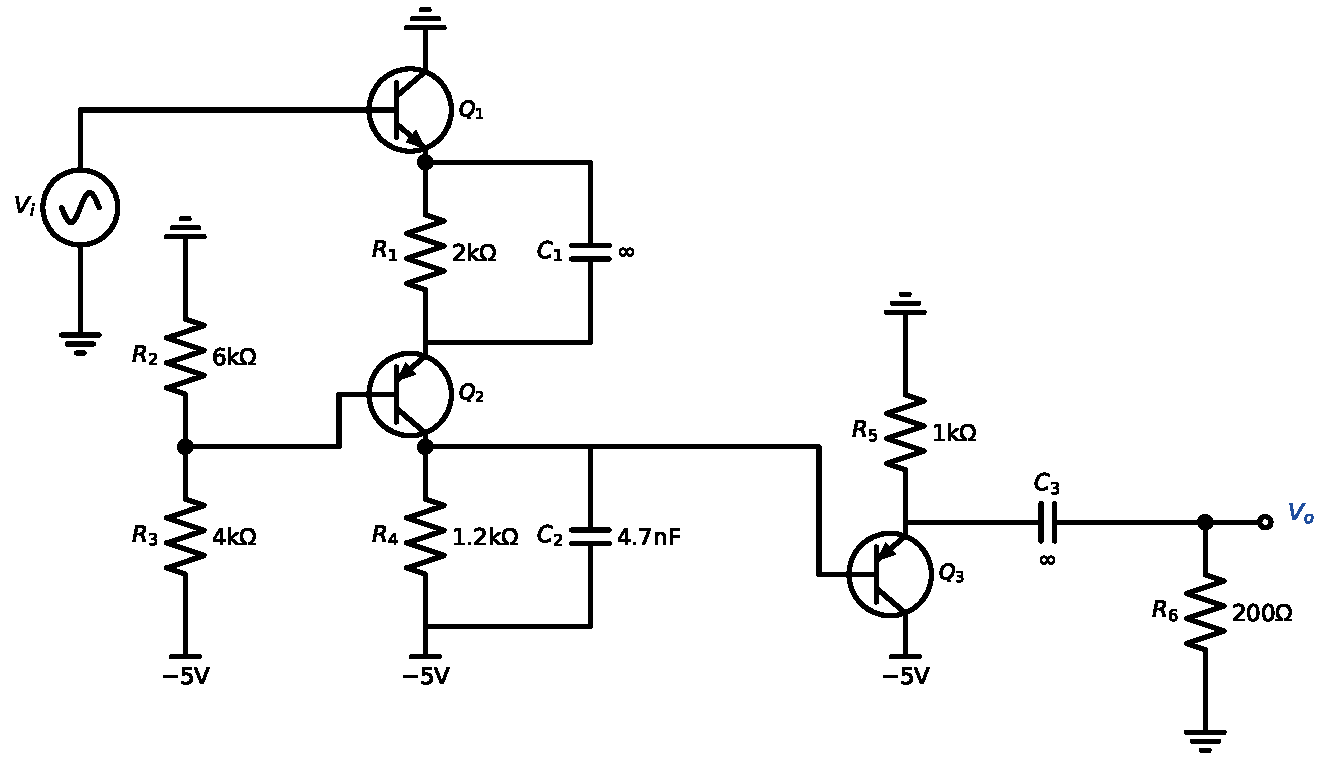
\includegraphics[width=\linewidth,height=7cm,keepaspectratio]{p14_circuit}\end{center}
\end{probbox}

\begin{probbox}{Problem 4D.15 \hfill Hard}
For the amplifier below, find the small-signal transfer function $H(s)=\dfrac{V_o(s)}{V_i(s)}$ and sketch its magnitude Bode plot. Also find the steady-state output $V_o(t)$ for $V_i(t) = 5\times 10^{-4}\sin\left(2\pi\cdot 2000\,t\right)$. $\beta = 100$, $V_T = 25$\,mV; the DC collector currents are $I_{C1} = 1\,\mathrm{m}\mathrm{A}$, $I_{C2} = 1\,\mathrm{m}\mathrm{A}$, $I_{C3} = 3\,\mathrm{m}\mathrm{A}$.
\begin{center}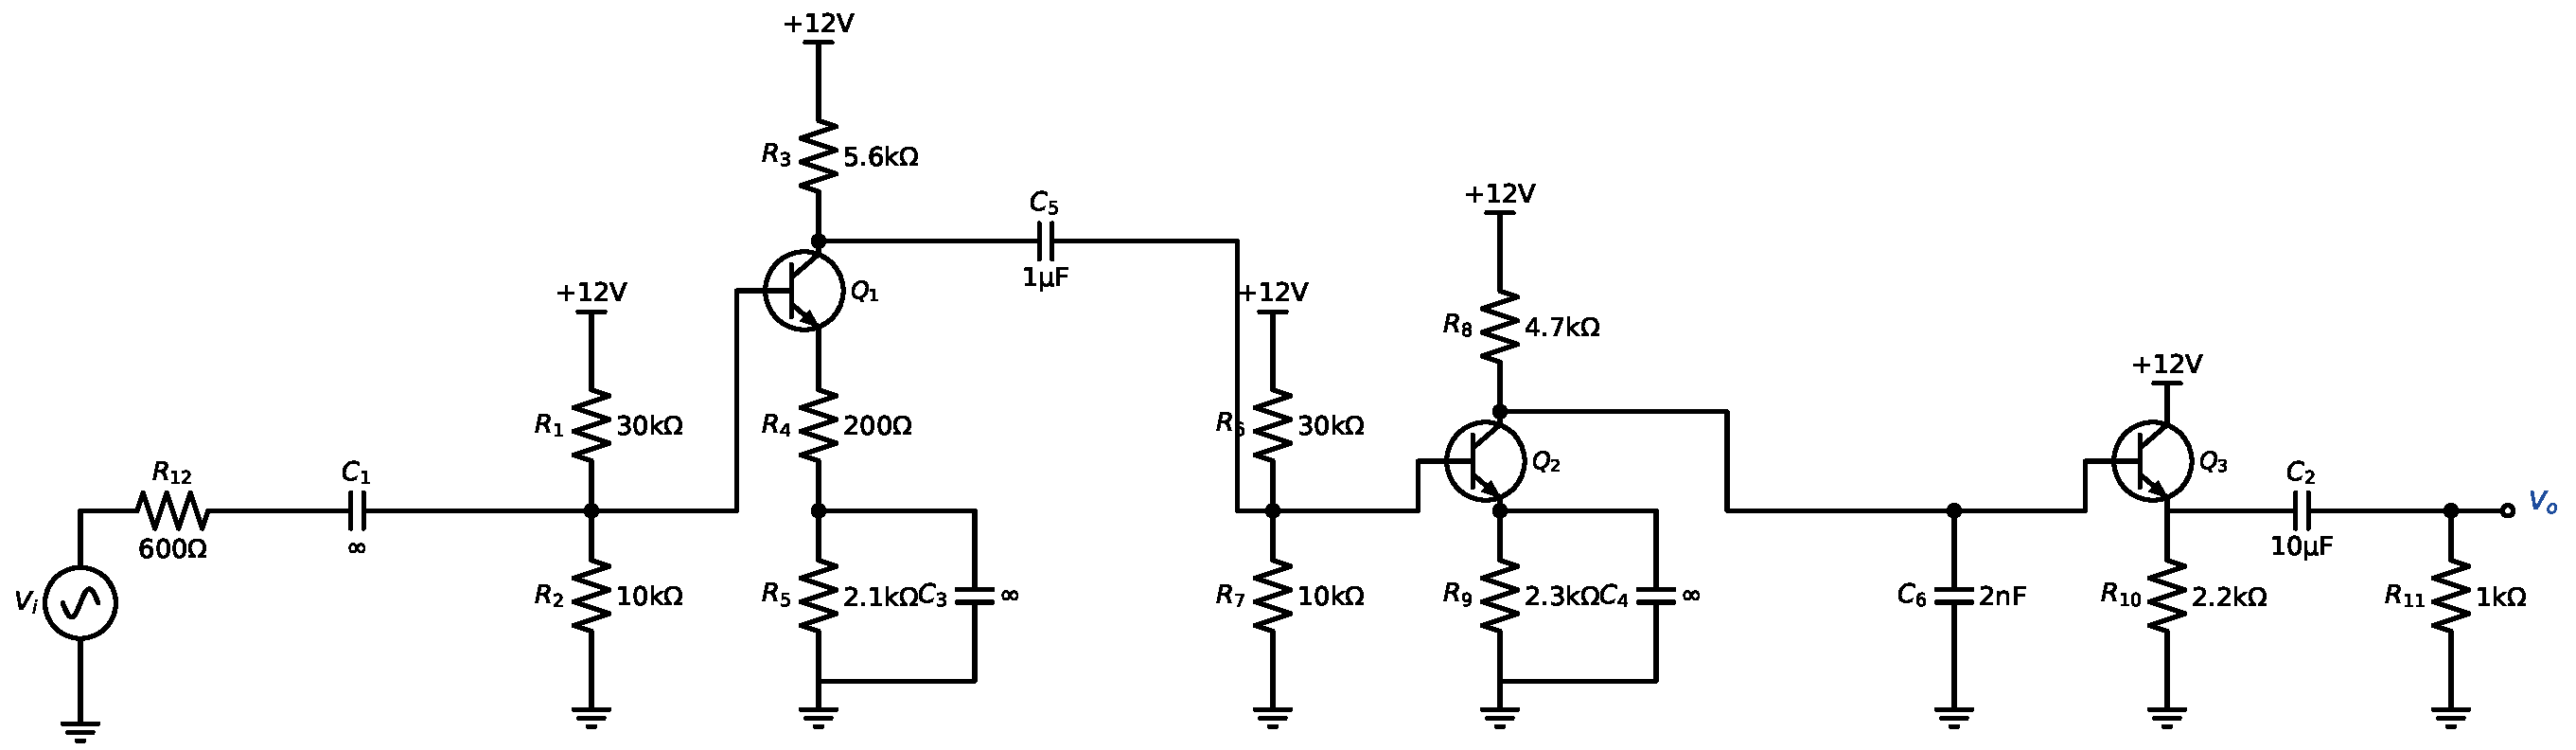
\includegraphics[width=\linewidth,height=7cm,keepaspectratio]{p15_circuit}\end{center}
\end{probbox}

\begin{probbox}{Problem 4D.16 \hfill Hard}
For the amplifier below, find the small-signal transfer function $H(s)=\dfrac{V_o(s)}{V_i(s)}$ and sketch its magnitude Bode plot. Also find the steady-state output $V_o(t)$ for $V_i(t) = 0.01\sin\left(2\pi\cdot 500\,t\right)$. $\beta = 100$, $V_T = 25$\,mV; the DC collector currents are $I_{C1} = 1\,\mathrm{m}\mathrm{A}$, $I_{C2} = 1.92\,\mathrm{m}\mathrm{A}$.
\begin{center}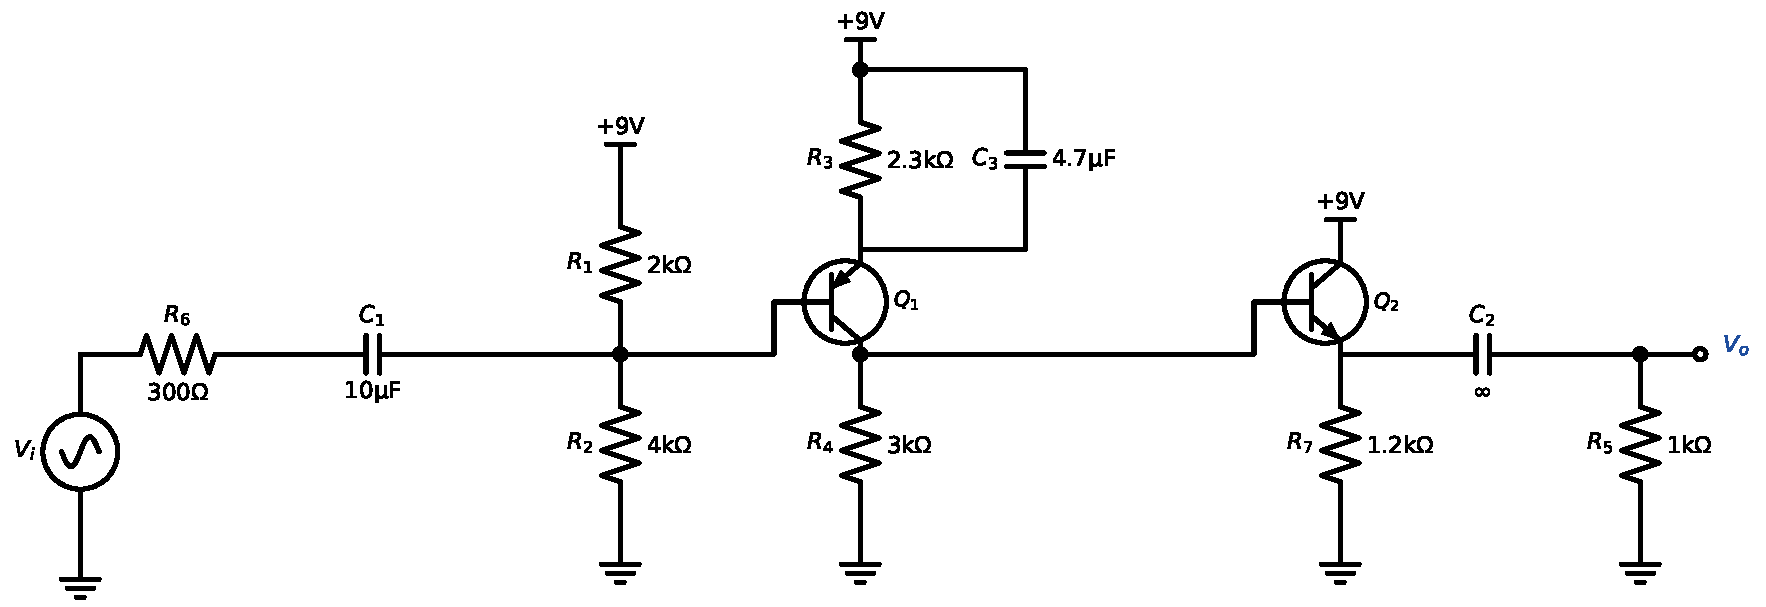
\includegraphics[width=\linewidth,height=7cm,keepaspectratio]{p16_circuit}\end{center}
\end{probbox}

\begin{probbox}{Problem 4D.17 \hfill Hard}
For the amplifier below, find the small-signal transfer function $H(s)=\dfrac{V_o(s)}{V_i(s)}$ and sketch its magnitude Bode plot. Also find the steady-state output $V_o(t)$ for $V_i(t) = 0.002\cos\left(2\pi\cdot 200\,t-\frac{\pi}{3}\right)$. $\beta = 100$, $V_T = 25$\,mV; the DC collector currents are $I_{C1} = 1.41\,\mathrm{m}\mathrm{A}$, $I_{C2} = 2.13\,\mathrm{m}\mathrm{A}$.
\begin{center}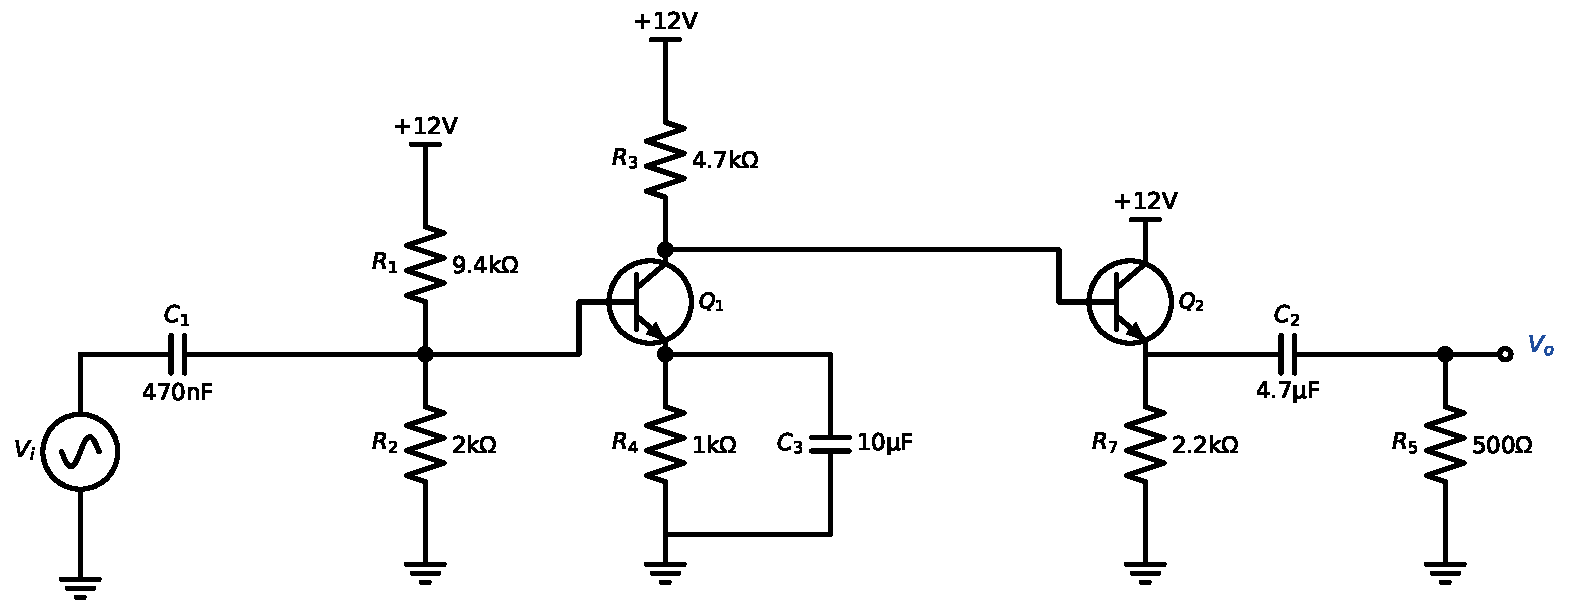
\includegraphics[width=\linewidth,height=7cm,keepaspectratio]{p17_circuit}\end{center}
\end{probbox}

\begin{probbox}{Problem 4D.18 \hfill Hard}
For the amplifier below, find the small-signal transfer function $H(s)=\dfrac{V_o(s)}{V_i(s)}$ and sketch its magnitude Bode plot. Also find the steady-state output $V_o(t)$ for $V_i(t) = 0.01\sin\left(2\pi\cdot 1000\,t\right)$. $\beta = 100$, $V_T = 25$\,mV; the DC collector currents are $I_{C1} = 1\,\mathrm{m}\mathrm{A}$, $I_{C2} = 1.73\,\mathrm{m}\mathrm{A}$, $I_{C3} = 3.56\,\mathrm{m}\mathrm{A}$.
\begin{center}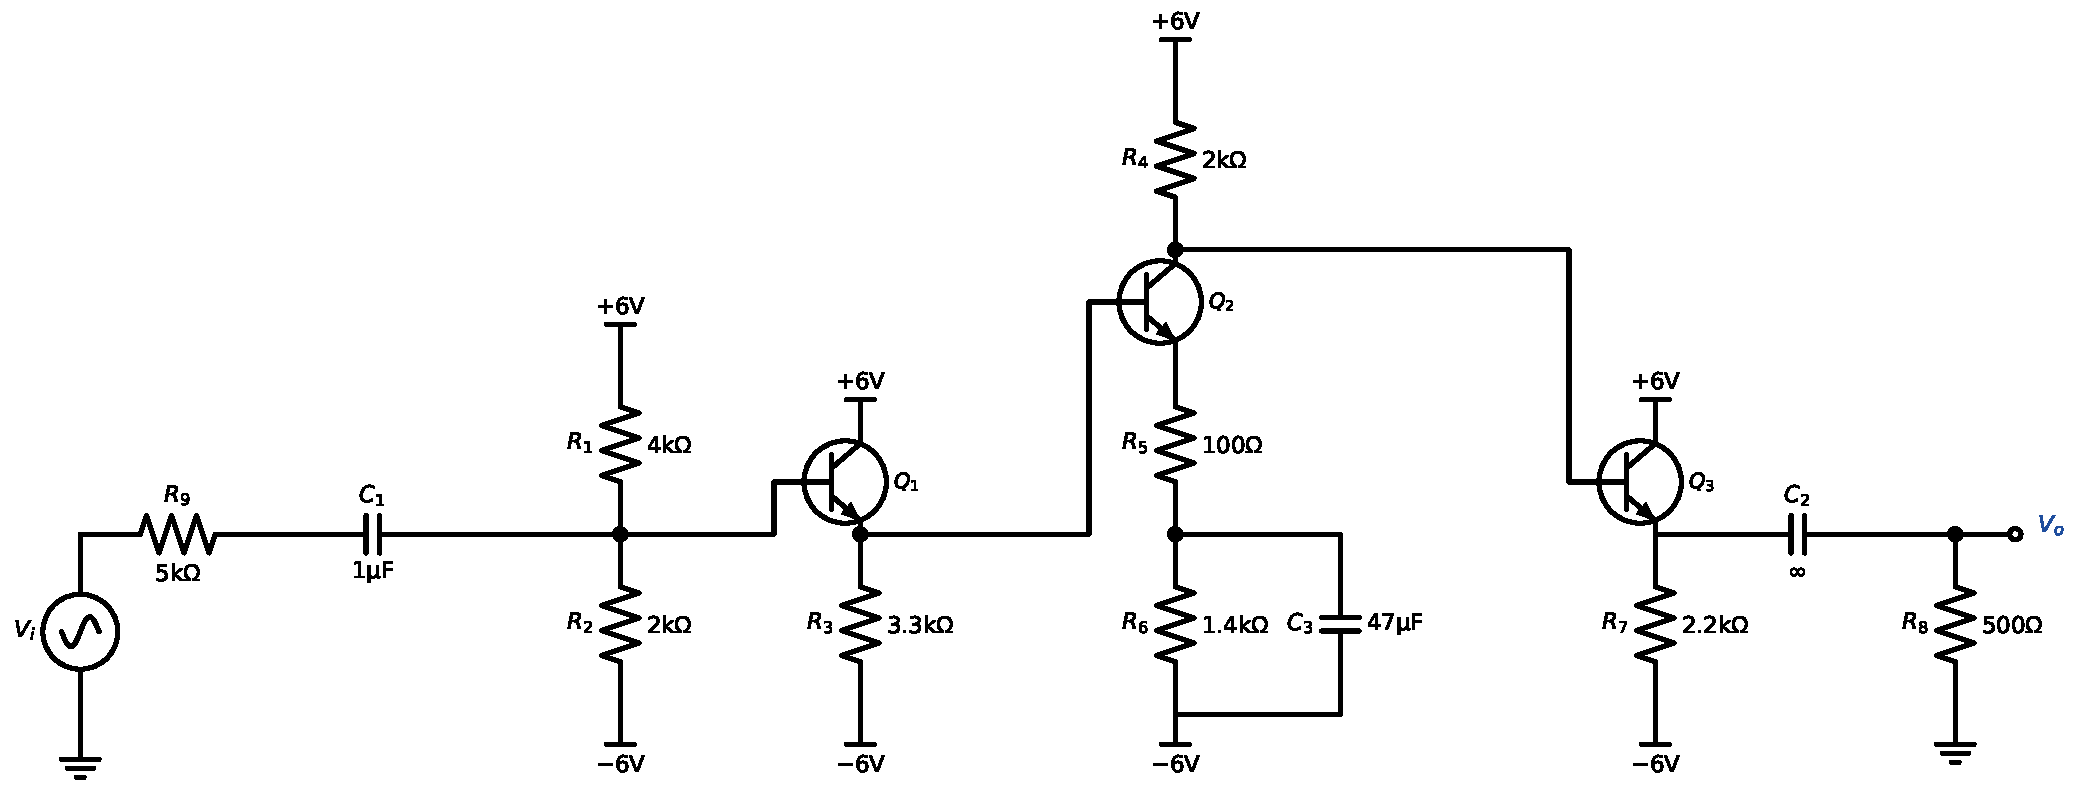
\includegraphics[width=\linewidth,height=7cm,keepaspectratio]{p18_circuit}\end{center}
\end{probbox}

\newpage
\section*{Solutions}
Every solution follows the steps of the Lecture-4 pipeline card.
\subsection*{Solution 4D.1 \hfill Easy}
\begin{center}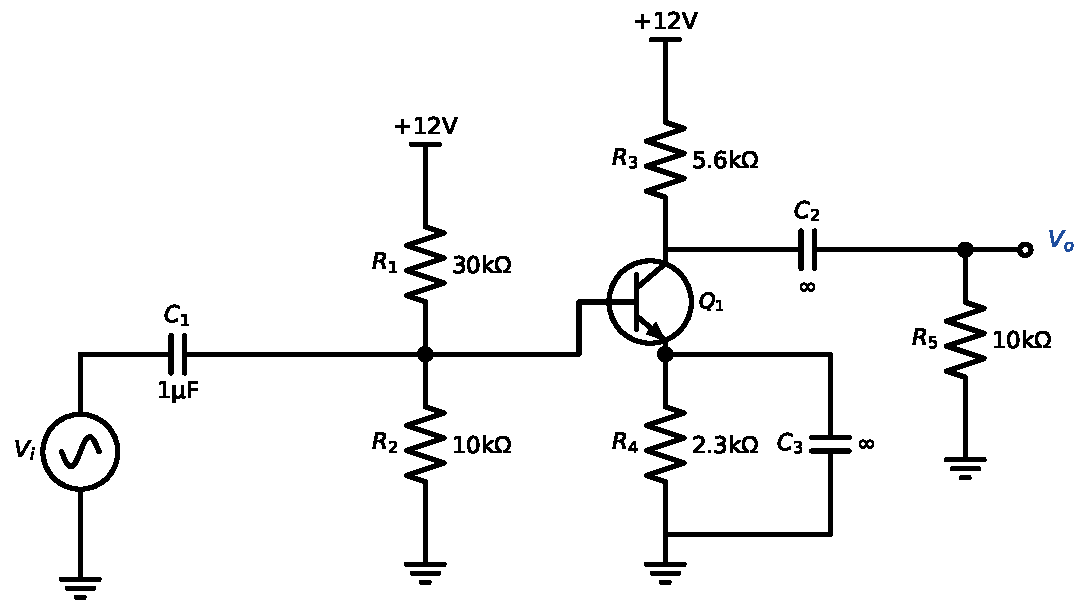
\includegraphics[width=0.9\linewidth,height=6cm,keepaspectratio]{p01_circuit}\end{center}
\solstep{1}{DC currents and small-signal parameters}The DC collector currents are given: $I_{C1} = 1\,\mathrm{m}\mathrm{A}$. For AC every DC supply is ground and every ``$\infty$'' capacitor is a short (tool T3). Small-signal emitter resistances (tool T3):\begin{align*}
r_{e1} &= \frac{V_T}{I_{C1}} = \frac{25\,\mathrm{mV}}{1\,\mathrm{m}\mathrm{A}} = 25\,\Omega
\end{align*}

\solstep{2}{Input resistance of each stage}Input resistance of every stage, from the last stage back to the first (each one loads the stage before it; tool T4):\begin{align*}
R_{i1} &= Z_{base,1} = (\beta+1)(r_{e1} + 0) = 2.52\,\mathrm{k}\Omega
\end{align*}

\solstep{3}{Gain along the signal path}Multiply the node-to-node gains along the signal path (tool T4):\[
H(s) = \frac{v_{b1}}{v_i}\cdot\frac{v_{c1}}{v_{b1}}
\]
\begin{align*}
\frac{v_{b1}}{v_i} &= \frac{R_{1} \parallel R_{2} \parallel R_{i1}}{\frac{1}{sC_{1}} + R_{1} \parallel R_{2} \parallel R_{i1}} = \dfrac{s}{s + 529} \\
\frac{v_{c1}}{v_{b1}} &= -\alpha\frac{Z_{C1}}{r_{e1} + Z_{E1}},\quad Z_{C1} = R_{3} \parallel R_{5},\ Z_{E1} = 0\ \Rightarrow\ -142
\end{align*}

\solstep{4}{Transfer function}Multiply and simplify:\[
H(s) = \dfrac{-142\,s}{s + 529}
\]

\solstep{5}{Standard (Bode-ready) form}Find the roots. Every root $s=-p$ of the denominator is a \emph{pole}, every root $s=-z$ of the numerator is a \emph{zero}; $|p|$ and $|z|$ are the corner frequencies (rad/s).
\begin{itemize}[leftmargin=*,itemsep=2pt]
\item Numerator: it has the factor $s$ $\Rightarrow$ 1 zero at $s=0$.
\item Denominator: $s + 529$; $s + 529 = 0 \Rightarrow s = -529$.
\end{itemize}

Factored form (leading coefficient in front):
\[
H(s) = -142\,\dfrac{s}{(s+529)}
\]

Bode-ready form: rewrite every $(s+p) = p\left(1+\frac{s}{p}\right)$ and $(s+z) = z\left(1+\frac{s}{z}\right)$, and collect all constants into $K$. Each $s$ in the numerator is paired with one of the \emph{lowest} poles as $\frac{s}{s+p}$ (that factor is $\approx 1$ above $p$). Then every factor except $K$ is $\approx 1$ inside the pass-band:
\[
H(s) = -142\,\dfrac{s}{s+2\pi\cdot 84.3},\qquad K = -142
\]

\begin{center}\renewcommand{\arraystretch}{1.35}
\begin{tabular}{cccc}
\toprule
type & $\omega_c$ (rad/s) & $f_c=\omega_c/2\pi$ & slope change \\
\midrule
pole & $529$ & 84.3 Hz & $-20$ dB/dec \\
\bottomrule
\end{tabular}\end{center}

\solstep{6}{Magnitude Bode plot}Below every corner $|H(s)|\approx 0.269\,s$, so the plot starts with a slope of $+20$\,dB/dec. Then, moving right, each pole bends the line down by 20\,dB/dec and each zero bends it up by 20\,dB/dec (tool T6):
\begin{center}\renewcommand{\arraystretch}{1.35}
\begin{tabular}{lcl}
\toprule
frequency range & slope & asymptote level \\
\midrule
$f<$ 84.3 Hz & $+20$ dB/dec & 43.1 dB at end \\
$f>$ 84.3 Hz & $0$ dB/dec (flat) & 43.1 dB at start \\
\bottomrule
\end{tabular}\end{center}

The flat (pass-band) level is $20\log_{10}|K| = 20\log_{10}142 = 43.1$\,dB.
\begin{center}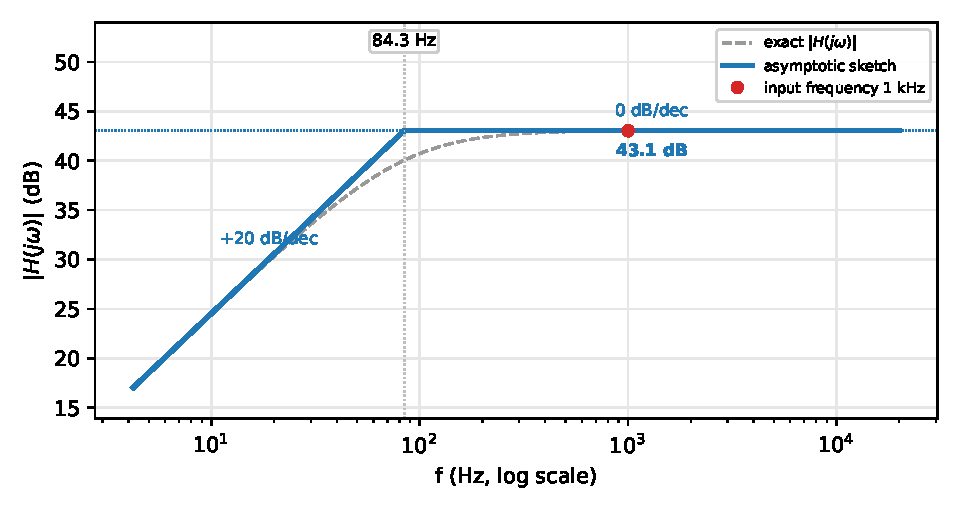
\includegraphics[width=0.78\linewidth,height=6.5cm,keepaspectratio]{p01_bode}\end{center}

{\small Blue: the straight-line sketch you are expected to draw. Dashed grey: the exact curve (about 3\,dB below the corner of an isolated pole). Red dot: the input frequency of Step 7.}
\solstep{7}{Steady-state output}The input is $V_i(t) = 0.005\sin\left(2\pi\cdot 1000\,t\right)$, so $\omega_{in} = 2\pi\cdot 1000 = 6280$\,rad/s. Put $s=j\omega_{in}$ in each factor (tool T5): magnitudes multiply, angles add.
{\small Rules: $\left|\frac{s}{s+p}\right| = \frac{\omega}{\sqrt{\omega^2+p^2}}$, $\angle = \frac{\pi}{2}-\tan^{-1}\frac{\omega}{p}$;\quad $\left|\frac{1}{1+s/p}\right| = \frac{1}{\sqrt{1+(\omega/p)^2}}$, $\angle = -\tan^{-1}\frac{\omega}{p}$;\quad $\left|1+\frac{s}{z}\right| = \sqrt{1+(\omega/z)^2}$, $\angle = \tan^{-1}\frac{\omega}{z}$;\quad a negative $K$ adds $-\pi$.}
\begin{center}\renewcommand{\arraystretch}{1.35}
\begin{tabular}{ccc}
\toprule
factor & magnitude & angle (rad) \\
\midrule
$-142$ & $142.2$ & $-3.14$ \\
$\rule[-1.1em]{0pt}{2.8em}\dfrac{s}{s+2\pi\cdot 84.3}$ & $0.9965$ & $0.0841$ \\
\textbf{total} & $\mathbf{141.7}$ (product) & $\mathbf{-3.06}$ (sum) \\
\bottomrule
\end{tabular}\end{center}

\begin{align*}
|H(j\omega_{in})| &= 142, \qquad \angle H(j\omega_{in}) = -3.06\ \mathrm{rad} \\
v_{o,ac}(t) &= 142\times 0.005\,\sin\left(2\pi\cdot 1000\,t - 3.06\right) = 0.708\,\sin\left(2\pi\cdot 1000\,t - 3.06\right)
\end{align*}

\[
\boxed{V_o(t) = 0.708\,\sin\left(2\pi\cdot 1000\,t - 3.06\right)\ \mathrm{V}}
\]

\begin{ansbox}
$H(s) = -142\,\dfrac{s}{s+2\pi\cdot 84.3}$\quad (corners: 84.3 Hz)\\[4pt]
$V_o(t) = 0.708\,\sin\left(2\pi\cdot 1000\,t - 3.06\right)\ \mathrm{V}$
\end{ansbox}

\newpage
\subsection*{Solution 4D.2 \hfill Easy}
\begin{center}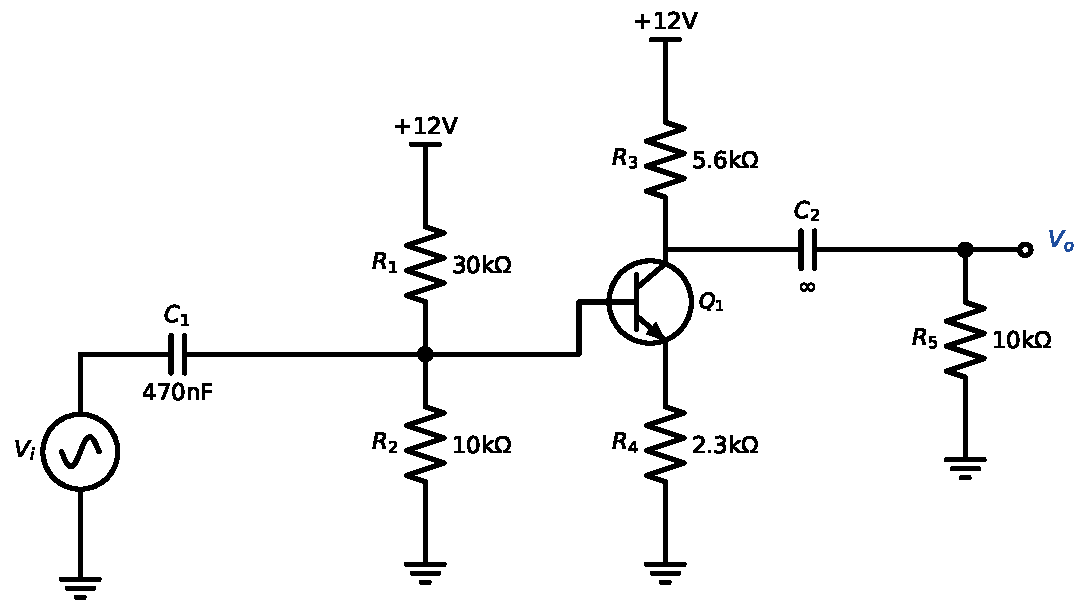
\includegraphics[width=0.9\linewidth,height=6cm,keepaspectratio]{p02_circuit}\end{center}
\solstep{1}{DC currents and small-signal parameters}The DC collector currents are given: $I_{C1} = 1\,\mathrm{m}\mathrm{A}$. For AC every DC supply is ground and every ``$\infty$'' capacitor is a short (tool T3). Small-signal emitter resistances (tool T3):\begin{align*}
r_{e1} &= \frac{V_T}{I_{C1}} = \frac{25\,\mathrm{mV}}{1\,\mathrm{m}\mathrm{A}} = 25\,\Omega
\end{align*}

\solstep{2}{Input resistance of each stage}Input resistance of every stage, from the last stage back to the first (each one loads the stage before it; tool T4):\begin{align*}
R_{i1} &= Z_{base,1} = (\beta+1)(r_{e1} + R_{4}) = 235\,\mathrm{k}\Omega
\end{align*}

\solstep{3}{Gain along the signal path}Multiply the node-to-node gains along the signal path (tool T4):\[
H(s) = \frac{v_{b1}}{v_i}\cdot\frac{v_{c1}}{v_{b1}}
\]
\begin{align*}
\frac{v_{b1}}{v_i} &= \frac{R_{1} \parallel R_{2} \parallel R_{i1}}{\frac{1}{sC_{1}} + R_{1} \parallel R_{2} \parallel R_{i1}} = \dfrac{s}{s + 293} \\
\frac{v_{c1}}{v_{b1}} &= -\alpha\frac{Z_{C1}}{r_{e1} + Z_{E1}},\quad Z_{C1} = R_{3} \parallel R_{5},\ Z_{E1} = R_{4}\ \Rightarrow\ -1.53
\end{align*}

\solstep{4}{Transfer function}Multiply and simplify:\[
H(s) = \dfrac{-1.53\,s}{s + 293}
\]

\solstep{5}{Standard (Bode-ready) form}Find the roots. Every root $s=-p$ of the denominator is a \emph{pole}, every root $s=-z$ of the numerator is a \emph{zero}; $|p|$ and $|z|$ are the corner frequencies (rad/s).
\begin{itemize}[leftmargin=*,itemsep=2pt]
\item Numerator: it has the factor $s$ $\Rightarrow$ 1 zero at $s=0$.
\item Denominator: $s + 293$; $s + 293 = 0 \Rightarrow s = -293$.
\end{itemize}

Factored form (leading coefficient in front):
\[
H(s) = -1.53\,\dfrac{s}{(s+293)}
\]

Bode-ready form: rewrite every $(s+p) = p\left(1+\frac{s}{p}\right)$ and $(s+z) = z\left(1+\frac{s}{z}\right)$, and collect all constants into $K$. Each $s$ in the numerator is paired with one of the \emph{lowest} poles as $\frac{s}{s+p}$ (that factor is $\approx 1$ above $p$). Then every factor except $K$ is $\approx 1$ inside the pass-band:
\[
H(s) = -1.53\,\dfrac{s}{s+2\pi\cdot 46.6},\qquad K = -1.53
\]

\begin{center}\renewcommand{\arraystretch}{1.35}
\begin{tabular}{cccc}
\toprule
type & $\omega_c$ (rad/s) & $f_c=\omega_c/2\pi$ & slope change \\
\midrule
pole & $293$ & 46.6 Hz & $-20$ dB/dec \\
\bottomrule
\end{tabular}\end{center}

\solstep{6}{Magnitude Bode plot}Below every corner $|H(s)|\approx 0.00522\,s$, so the plot starts with a slope of $+20$\,dB/dec. Then, moving right, each pole bends the line down by 20\,dB/dec and each zero bends it up by 20\,dB/dec (tool T6):
\begin{center}\renewcommand{\arraystretch}{1.35}
\begin{tabular}{lcl}
\toprule
frequency range & slope & asymptote level \\
\midrule
$f<$ 46.6 Hz & $+20$ dB/dec & 3.69 dB at end \\
$f>$ 46.6 Hz & $0$ dB/dec (flat) & 3.69 dB at start \\
\bottomrule
\end{tabular}\end{center}

The flat (pass-band) level is $20\log_{10}|K| = 20\log_{10}1.53 = 3.69$\,dB.
\begin{center}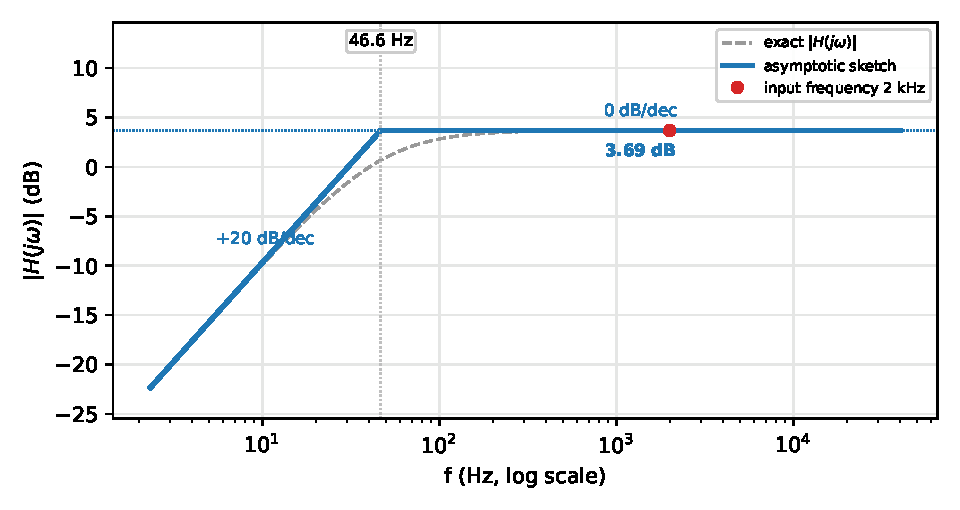
\includegraphics[width=0.78\linewidth,height=6.5cm,keepaspectratio]{p02_bode}\end{center}

{\small Blue: the straight-line sketch you are expected to draw. Dashed grey: the exact curve (about 3\,dB below the corner of an isolated pole). Red dot: the input frequency of Step 7.}
\solstep{7}{Steady-state output}The input is $V_i(t) = 0.05\sin\left(2\pi\cdot 2000\,t\right)$, so $\omega_{in} = 2\pi\cdot 2000 = 12600$\,rad/s. Put $s=j\omega_{in}$ in each factor (tool T5): magnitudes multiply, angles add.
{\small Rules: $\left|\frac{s}{s+p}\right| = \frac{\omega}{\sqrt{\omega^2+p^2}}$, $\angle = \frac{\pi}{2}-\tan^{-1}\frac{\omega}{p}$;\quad $\left|\frac{1}{1+s/p}\right| = \frac{1}{\sqrt{1+(\omega/p)^2}}$, $\angle = -\tan^{-1}\frac{\omega}{p}$;\quad $\left|1+\frac{s}{z}\right| = \sqrt{1+(\omega/z)^2}$, $\angle = \tan^{-1}\frac{\omega}{z}$;\quad a negative $K$ adds $-\pi$.}
\begin{center}\renewcommand{\arraystretch}{1.35}
\begin{tabular}{ccc}
\toprule
factor & magnitude & angle (rad) \\
\midrule
$-1.53$ & $1.529$ & $-3.14$ \\
$\rule[-1.1em]{0pt}{2.8em}\dfrac{s}{s+2\pi\cdot 46.6}$ & $0.9997$ & $0.0233$ \\
\textbf{total} & $\mathbf{1.528}$ (product) & $\mathbf{-3.12}$ (sum) \\
\bottomrule
\end{tabular}\end{center}

\begin{align*}
|H(j\omega_{in})| &= 1.53, \qquad \angle H(j\omega_{in}) = -3.12\ \mathrm{rad} \\
v_{o,ac}(t) &= 1.53\times 0.05\,\sin\left(2\pi\cdot 2000\,t - 3.12\right) = 0.0764\,\sin\left(2\pi\cdot 2000\,t - 3.12\right)
\end{align*}

\[
\boxed{V_o(t) = 0.0764\,\sin\left(2\pi\cdot 2000\,t - 3.12\right)\ \mathrm{V}}
\]

\begin{ansbox}
$H(s) = -1.53\,\dfrac{s}{s+2\pi\cdot 46.6}$\quad (corners: 46.6 Hz)\\[4pt]
$V_o(t) = 0.0764\,\sin\left(2\pi\cdot 2000\,t - 3.12\right)\ \mathrm{V}$
\end{ansbox}

\newpage
\subsection*{Solution 4D.3 \hfill Easy}
\begin{center}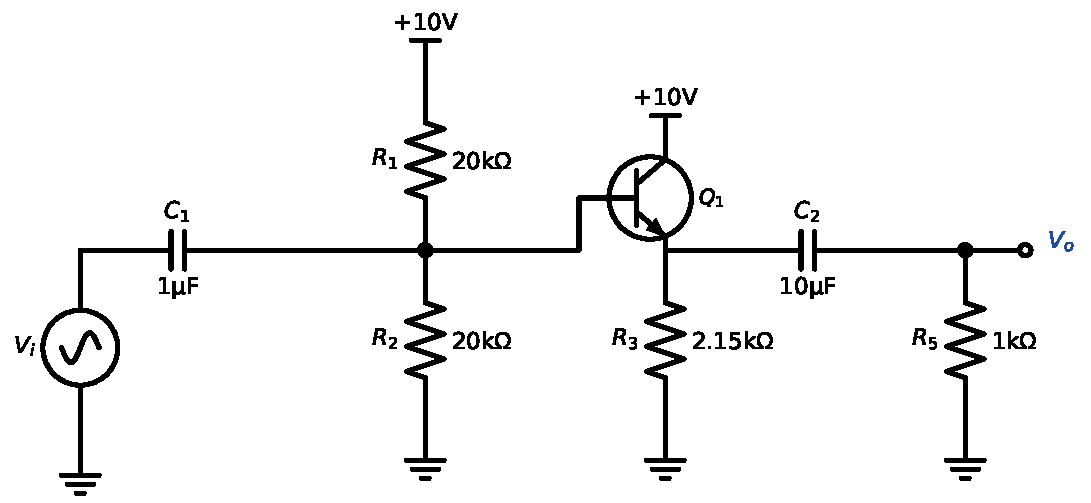
\includegraphics[width=0.9\linewidth,height=6cm,keepaspectratio]{p03_circuit}\end{center}
\solstep{1}{DC currents and small-signal parameters}The DC collector currents are given: $I_{C1} = 2\,\mathrm{m}\mathrm{A}$. For AC every DC supply is ground and every ``$\infty$'' capacitor is a short (tool T3). Small-signal emitter resistances (tool T3):\begin{align*}
r_{e1} &= \frac{V_T}{I_{C1}} = \frac{25\,\mathrm{mV}}{2\,\mathrm{m}\mathrm{A}} = 12.5\,\Omega
\end{align*}

\solstep{2}{Input resistance of each stage}Input resistance of every stage, from the last stage back to the first (each one loads the stage before it; tool T4):\begin{align*}
R_{i1} &= Z_{base,1} = (\beta+1)(r_{e1} + R_{3} \parallel \left(\frac{1}{sC_{2}} + R_{5}\right)) = \dfrac{70200\,s + 6.93\times 10^{6}}{s + 31.7}
\end{align*}

\solstep{3}{Gain along the signal path}Multiply the node-to-node gains along the signal path (tool T4):\[
H(s) = \frac{v_{b1}}{v_i}\cdot\frac{v_{e1}}{v_{b1}}\cdot\frac{v_o}{v_{e1}}
\]
\begin{align*}
\frac{v_{b1}}{v_i} &= \frac{R_{1} \parallel R_{2} \parallel R_{i1}}{\frac{1}{sC_{1}} + R_{1} \parallel R_{2} \parallel R_{i1}} = \dfrac{s^{2} + 98.8\,s}{s^{2} + 213\,s + 10300} \\
\frac{v_{e1}}{v_{b1}} &= \frac{Z_{E1}}{r_{e1} + Z_{E1}},\quad Z_{E1} = R_{3} \parallel \left(\frac{1}{sC_{2}} + R_{5}\right)\ \Rightarrow\ \dfrac{0.982\,s + 98.2}{s + 98.8} \\
\frac{v_o}{v_{e1}} &= \frac{R_{5}}{\frac{1}{sC_{2}} + R_{5}} = \dfrac{s}{s + 100}
\end{align*}

\solstep{4}{Transfer function}Multiply and simplify:\[
H(s) = \dfrac{0.982\,s^{2}}{s^{2} + 213\,s + 10300}
\]

\solstep{5}{Standard (Bode-ready) form}Find the roots. Every root $s=-p$ of the denominator is a \emph{pole}, every root $s=-z$ of the numerator is a \emph{zero}; $|p|$ and $|z|$ are the corner frequencies (rad/s).
\begin{itemize}[leftmargin=*,itemsep=2pt]
\item Numerator: it has the factor $s^2$ $\Rightarrow$ 2 zeros at $s=0$.
\item Denominator: $s^{2} + 213\,s + 10300$; quadratic formula:\[
s = \frac{-213 \pm \sqrt{(213)^2 - 4(10300)}}{2} = \frac{-213 \pm 63.7}{2} \Rightarrow s = -74.7,\ -138
\]

\end{itemize}

Factored form (leading coefficient in front):
\[
H(s) = 0.982\,\dfrac{s^{2}}{(s+74.7)(s+138)}
\]

Bode-ready form: rewrite every $(s+p) = p\left(1+\frac{s}{p}\right)$ and $(s+z) = z\left(1+\frac{s}{z}\right)$, and collect all constants into $K$. Each $s$ in the numerator is paired with one of the \emph{lowest} poles as $\frac{s}{s+p}$ (that factor is $\approx 1$ above $p$). Then every factor except $K$ is $\approx 1$ inside the pass-band:
\[
H(s) = 0.982\,\dfrac{s}{s+2\pi\cdot 11.9}\,\dfrac{s}{s+2\pi\cdot 22},\qquad K = 0.982
\]

\begin{center}\renewcommand{\arraystretch}{1.35}
\begin{tabular}{cccc}
\toprule
type & $\omega_c$ (rad/s) & $f_c=\omega_c/2\pi$ & slope change \\
\midrule
pole & $74.7$ & 11.9 Hz & $-20$ dB/dec \\
pole & $138$ & 22 Hz & $-20$ dB/dec \\
\bottomrule
\end{tabular}\end{center}

\solstep{6}{Magnitude Bode plot}Below every corner $|H(s)|\approx 9.51\times 10^{-5}\,s^2$, so the plot starts with a slope of $+40$\,dB/dec. Then, moving right, each pole bends the line down by 20\,dB/dec and each zero bends it up by 20\,dB/dec (tool T6):
\begin{center}\renewcommand{\arraystretch}{1.35}
\begin{tabular}{lcl}
\toprule
frequency range & slope & asymptote level \\
\midrule
$f<$ 11.9 Hz & $+40$ dB/dec & -5.52 dB at end \\
11.9 Hz -- 22 Hz & $+20$ dB/dec & -5.52 dB at start, -0.158 dB at end \\
$f>$ 22 Hz & $0$ dB/dec (flat) & -0.158 dB at start \\
\bottomrule
\end{tabular}\end{center}

The flat (pass-band) level is $20\log_{10}|K| = 20\log_{10}0.982 = -0.158$\,dB.
\begin{center}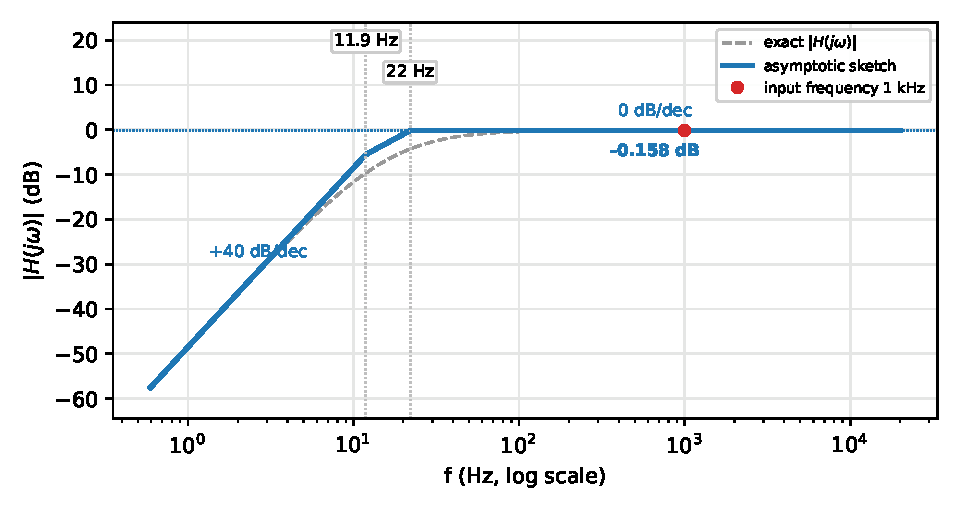
\includegraphics[width=0.78\linewidth,height=6.5cm,keepaspectratio]{p03_bode}\end{center}

{\small Blue: the straight-line sketch you are expected to draw. Dashed grey: the exact curve (about 3\,dB below the corner of an isolated pole). Red dot: the input frequency of Step 7.}
\solstep{7}{Steady-state output}The input is $V_i(t) = 0.5\sin\left(2\pi\cdot 1000\,t\right)$, so $\omega_{in} = 2\pi\cdot 1000 = 6280$\,rad/s. Put $s=j\omega_{in}$ in each factor (tool T5): magnitudes multiply, angles add.
{\small Rules: $\left|\frac{s}{s+p}\right| = \frac{\omega}{\sqrt{\omega^2+p^2}}$, $\angle = \frac{\pi}{2}-\tan^{-1}\frac{\omega}{p}$;\quad $\left|\frac{1}{1+s/p}\right| = \frac{1}{\sqrt{1+(\omega/p)^2}}$, $\angle = -\tan^{-1}\frac{\omega}{p}$;\quad $\left|1+\frac{s}{z}\right| = \sqrt{1+(\omega/z)^2}$, $\angle = \tan^{-1}\frac{\omega}{z}$;\quad a negative $K$ adds $-\pi$.}
\begin{center}\renewcommand{\arraystretch}{1.35}
\begin{tabular}{ccc}
\toprule
factor & magnitude & angle (rad) \\
\midrule
$0.982$ & $0.982$ & $0$ \\
$\rule[-1.1em]{0pt}{2.8em}\dfrac{s}{s+2\pi\cdot 11.9}$ & $0.9999$ & $0.0119$ \\
$\rule[-1.1em]{0pt}{2.8em}\dfrac{s}{s+2\pi\cdot 22}$ & $0.9998$ & $0.022$ \\
\textbf{total} & $\mathbf{0.9817}$ (product) & $\mathbf{0.0339}$ (sum) \\
\bottomrule
\end{tabular}\end{center}

\begin{align*}
|H(j\omega_{in})| &= 0.982, \qquad \angle H(j\omega_{in}) = 0.0339\ \mathrm{rad} \\
v_{o,ac}(t) &= 0.982\times 0.5\,\sin\left(2\pi\cdot 1000\,t + 0.0339\right) = 0.491\,\sin\left(2\pi\cdot 1000\,t + 0.0339\right)
\end{align*}

\[
\boxed{V_o(t) = 0.491\,\sin\left(2\pi\cdot 1000\,t + 0.0339\right)\ \mathrm{V}}
\]

\begin{ansbox}
$H(s) = 0.982\,\dfrac{s}{s+2\pi\cdot 11.9}\,\dfrac{s}{s+2\pi\cdot 22}$\quad (corners: 11.9 Hz, 22 Hz)\\[4pt]
$V_o(t) = 0.491\,\sin\left(2\pi\cdot 1000\,t + 0.0339\right)\ \mathrm{V}$
\end{ansbox}

\newpage
\subsection*{Solution 4D.4 \hfill Easy}
\begin{center}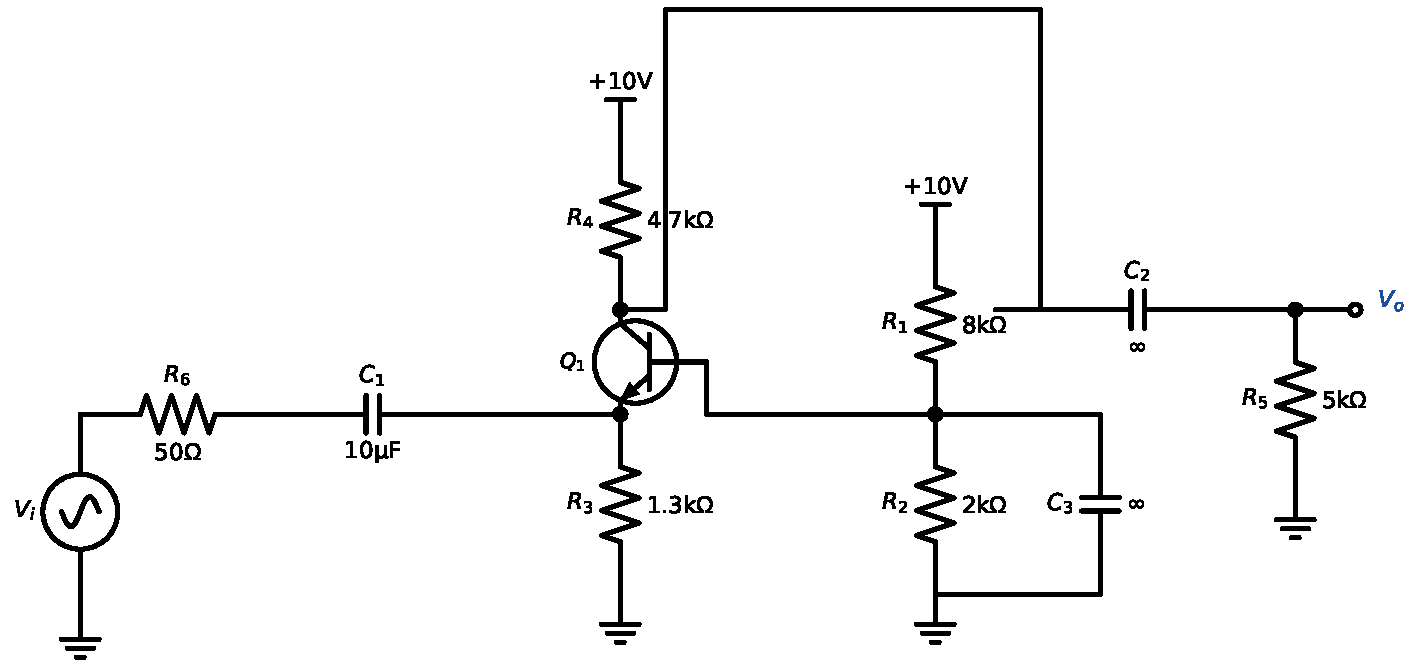
\includegraphics[width=0.9\linewidth,height=6cm,keepaspectratio]{p04_circuit}\end{center}
\solstep{1}{DC currents and small-signal parameters}The DC collector currents are given: $I_{C1} = 1\,\mathrm{m}\mathrm{A}$. For AC every DC supply is ground and every ``$\infty$'' capacitor is a short (tool T3). Small-signal emitter resistances (tool T3):\begin{align*}
r_{e1} &= \frac{V_T}{I_{C1}} = \frac{25\,\mathrm{mV}}{1\,\mathrm{m}\mathrm{A}} = 25\,\Omega
\end{align*}

\solstep{2}{Input resistance of each stage}Input resistance of every stage, from the last stage back to the first (each one loads the stage before it; tool T4):\begin{align*}
R_{i1} &= Z_{emitter,1} = r_{e1} + \frac{0}{\beta+1} = 25\,\Omega
\end{align*}

\solstep{3}{Gain along the signal path}Multiply the node-to-node gains along the signal path (tool T4):\[
H(s) = \frac{v_{e1}}{v_i}\cdot\frac{v_{c1}}{v_{e1}}
\]
\begin{align*}
\frac{v_{e1}}{v_i} &= \frac{R_{3} \parallel R_{i1}}{R_{6} + \frac{1}{sC_{1}} + R_{3} \parallel R_{i1}} = \dfrac{0.329\,s}{s + 1340} \\
\frac{v_{c1}}{v_{e1}} &= \alpha\frac{Z_{C1}}{Z_{emitter,1}},\quad Z_{C1} = R_{4} \parallel R_{5}\ \Rightarrow\ 95.9
\end{align*}

\solstep{4}{Transfer function}Multiply and simplify:\[
H(s) = \dfrac{31.6\,s}{s + 1340}
\]

\solstep{5}{Standard (Bode-ready) form}Find the roots. Every root $s=-p$ of the denominator is a \emph{pole}, every root $s=-z$ of the numerator is a \emph{zero}; $|p|$ and $|z|$ are the corner frequencies (rad/s).
\begin{itemize}[leftmargin=*,itemsep=2pt]
\item Numerator: it has the factor $s$ $\Rightarrow$ 1 zero at $s=0$.
\item Denominator: $s + 1340$; $s + 1340 = 0 \Rightarrow s = -1340$.
\end{itemize}

Factored form (leading coefficient in front):
\[
H(s) = 31.6\,\dfrac{s}{(s+1340)}
\]

Bode-ready form: rewrite every $(s+p) = p\left(1+\frac{s}{p}\right)$ and $(s+z) = z\left(1+\frac{s}{z}\right)$, and collect all constants into $K$. Each $s$ in the numerator is paired with one of the \emph{lowest} poles as $\frac{s}{s+p}$ (that factor is $\approx 1$ above $p$). Then every factor except $K$ is $\approx 1$ inside the pass-band:
\[
H(s) = 31.6\,\dfrac{s}{s+2\pi\cdot 214},\qquad K = 31.6
\]

\begin{center}\renewcommand{\arraystretch}{1.35}
\begin{tabular}{cccc}
\toprule
type & $\omega_c$ (rad/s) & $f_c=\omega_c/2\pi$ & slope change \\
\midrule
pole & $1340$ & 214 Hz & $-20$ dB/dec \\
\bottomrule
\end{tabular}\end{center}

\solstep{6}{Magnitude Bode plot}Below every corner $|H(s)|\approx 0.0235\,s$, so the plot starts with a slope of $+20$\,dB/dec. Then, moving right, each pole bends the line down by 20\,dB/dec and each zero bends it up by 20\,dB/dec (tool T6):
\begin{center}\renewcommand{\arraystretch}{1.35}
\begin{tabular}{lcl}
\toprule
frequency range & slope & asymptote level \\
\midrule
$f<$ 214 Hz & $+20$ dB/dec & 30 dB at end \\
$f>$ 214 Hz & $0$ dB/dec (flat) & 30 dB at start \\
\bottomrule
\end{tabular}\end{center}

The flat (pass-band) level is $20\log_{10}|K| = 20\log_{10}31.6 = 30$\,dB.
\begin{center}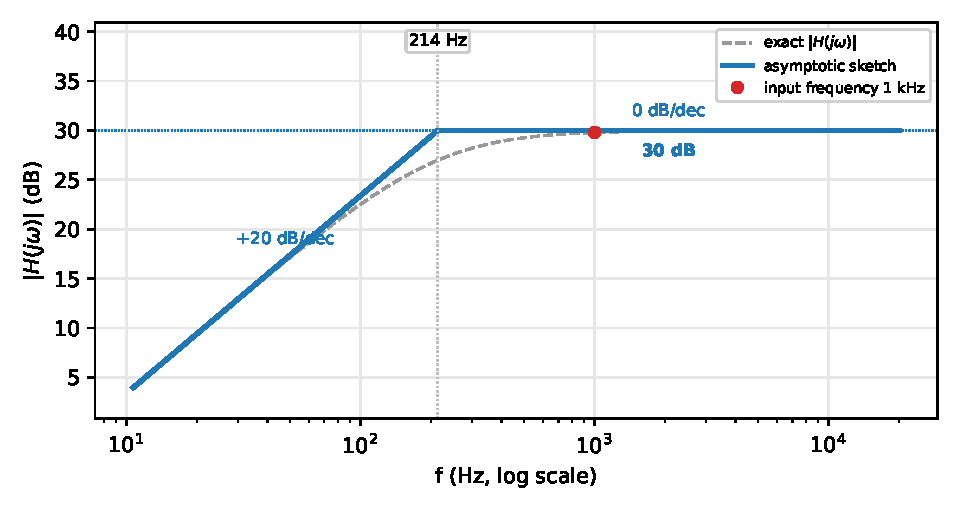
\includegraphics[width=0.78\linewidth,height=6.5cm,keepaspectratio]{p04_bode}\end{center}

{\small Blue: the straight-line sketch you are expected to draw. Dashed grey: the exact curve (about 3\,dB below the corner of an isolated pole). Red dot: the input frequency of Step 7.}
\solstep{7}{Steady-state output}The input is $V_i(t) = 0.01\sin\left(2\pi\cdot 1000\,t\right)$, so $\omega_{in} = 2\pi\cdot 1000 = 6280$\,rad/s. Put $s=j\omega_{in}$ in each factor (tool T5): magnitudes multiply, angles add.
{\small Rules: $\left|\frac{s}{s+p}\right| = \frac{\omega}{\sqrt{\omega^2+p^2}}$, $\angle = \frac{\pi}{2}-\tan^{-1}\frac{\omega}{p}$;\quad $\left|\frac{1}{1+s/p}\right| = \frac{1}{\sqrt{1+(\omega/p)^2}}$, $\angle = -\tan^{-1}\frac{\omega}{p}$;\quad $\left|1+\frac{s}{z}\right| = \sqrt{1+(\omega/z)^2}$, $\angle = \tan^{-1}\frac{\omega}{z}$;\quad a negative $K$ adds $-\pi$.}
\begin{center}\renewcommand{\arraystretch}{1.35}
\begin{tabular}{ccc}
\toprule
factor & magnitude & angle (rad) \\
\midrule
$31.6$ & $31.58$ & $0$ \\
$\rule[-1.1em]{0pt}{2.8em}\dfrac{s}{s+2\pi\cdot 214}$ & $0.9779$ & $0.21$ \\
\textbf{total} & $\mathbf{30.88}$ (product) & $\mathbf{0.21}$ (sum) \\
\bottomrule
\end{tabular}\end{center}

\begin{align*}
|H(j\omega_{in})| &= 30.9, \qquad \angle H(j\omega_{in}) = 0.21\ \mathrm{rad} \\
v_{o,ac}(t) &= 30.9\times 0.01\,\sin\left(2\pi\cdot 1000\,t + 0.21\right) = 0.309\,\sin\left(2\pi\cdot 1000\,t + 0.21\right)
\end{align*}

\[
\boxed{V_o(t) = 0.309\,\sin\left(2\pi\cdot 1000\,t + 0.21\right)\ \mathrm{V}}
\]

\begin{ansbox}
$H(s) = 31.6\,\dfrac{s}{s+2\pi\cdot 214}$\quad (corners: 214 Hz)\\[4pt]
$V_o(t) = 0.309\,\sin\left(2\pi\cdot 1000\,t + 0.21\right)\ \mathrm{V}$
\end{ansbox}

\newpage
\subsection*{Solution 4D.5 \hfill Easy}
\begin{center}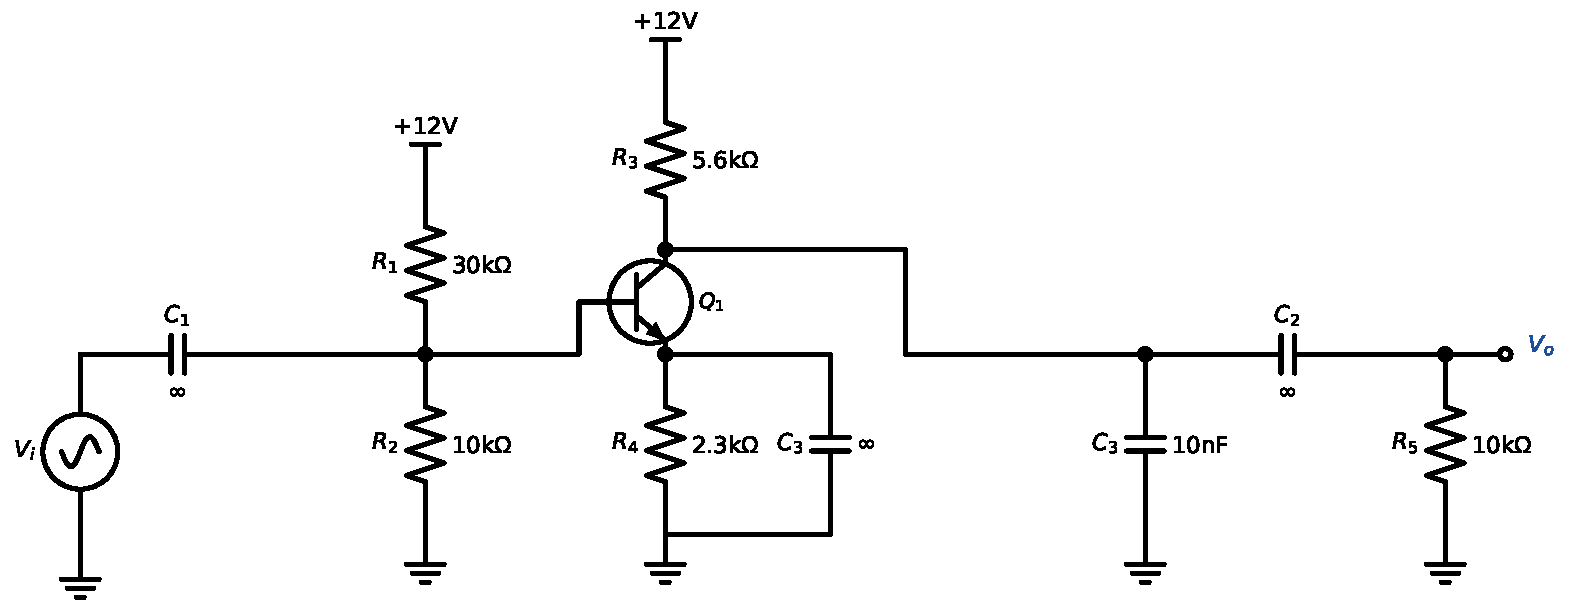
\includegraphics[width=0.9\linewidth,height=6cm,keepaspectratio]{p05_circuit}\end{center}
\solstep{1}{DC currents and small-signal parameters}The DC collector currents are given: $I_{C1} = 1\,\mathrm{m}\mathrm{A}$. For AC every DC supply is ground and every ``$\infty$'' capacitor is a short (tool T3). Small-signal emitter resistances (tool T3):\begin{align*}
r_{e1} &= \frac{V_T}{I_{C1}} = \frac{25\,\mathrm{mV}}{1\,\mathrm{m}\mathrm{A}} = 25\,\Omega
\end{align*}

\solstep{2}{Input resistance of each stage}Input resistance of every stage, from the last stage back to the first (each one loads the stage before it; tool T4):\begin{align*}
R_{i1} &= Z_{base,1} = (\beta+1)(r_{e1} + 0) = 2.52\,\mathrm{k}\Omega
\end{align*}

\solstep{3}{Gain along the signal path}Multiply the node-to-node gains along the signal path (tool T4):\[
H(s) = \frac{v_{c1}}{v_{b1}}
\]
\begin{align*}
\frac{v_{c1}}{v_{b1}} &= -\alpha\frac{Z_{C1}}{r_{e1} + Z_{E1}},\quad Z_{C1} = R_{3} \parallel \frac{1}{sC_{3}} \parallel R_{5},\ Z_{E1} = 0\ \Rightarrow\ \dfrac{-3.96\times 10^{6}}{s + 27900}
\end{align*}

\solstep{4}{Transfer function}Multiply and simplify:\[
H(s) = \dfrac{-3.96\times 10^{6}}{s + 27900}
\]

\solstep{5}{Standard (Bode-ready) form}Find the roots. Every root $s=-p$ of the denominator is a \emph{pole}, every root $s=-z$ of the numerator is a \emph{zero}; $|p|$ and $|z|$ are the corner frequencies (rad/s).
\begin{itemize}[leftmargin=*,itemsep=2pt]
\item Denominator: $s + 27900$; $s + 27900 = 0 \Rightarrow s = -27900$.
\end{itemize}

Factored form (leading coefficient in front):
\[
H(s) = -3.96\times 10^{6}\,\dfrac{1}{(s+27900)}
\]

Bode-ready form: rewrite every $(s+p) = p\left(1+\frac{s}{p}\right)$ and $(s+z) = z\left(1+\frac{s}{z}\right)$, and collect all constants into $K$. Then every factor except $K$ is $\approx 1$ inside the pass-band:
\[
H(s) = -142\,\dfrac{1}{1+\dfrac{s}{2\pi\cdot 4.43\mathrm{k}}},\qquad K = -142
\]

\begin{center}\renewcommand{\arraystretch}{1.35}
\begin{tabular}{cccc}
\toprule
type & $\omega_c$ (rad/s) & $f_c=\omega_c/2\pi$ & slope change \\
\midrule
pole & $27900$ & 4.43 kHz & $-20$ dB/dec \\
\bottomrule
\end{tabular}\end{center}

\solstep{6}{Magnitude Bode plot}Below every corner, all factors are $\approx$ constant: $|H| \approx 142$ $= 43.1$\,dB (flat, 0 dB/dec). Then, moving right, each pole bends the line down by 20\,dB/dec and each zero bends it up by 20\,dB/dec (tool T6):
\begin{center}\renewcommand{\arraystretch}{1.35}
\begin{tabular}{lcl}
\toprule
frequency range & slope & asymptote level \\
\midrule
$f<$ 4.43 kHz & $0$ dB/dec (flat) & 43.1 dB at end \\
$f>$ 4.43 kHz & $-20$ dB/dec & 43.1 dB at start \\
\bottomrule
\end{tabular}\end{center}

The flat (pass-band) level is $20\log_{10}|K| = 20\log_{10}142 = 43.1$\,dB.
\begin{center}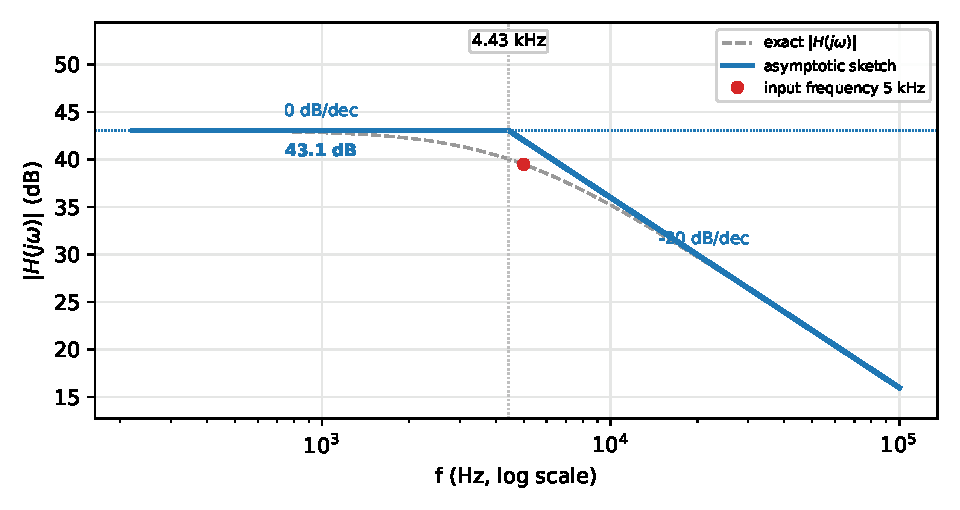
\includegraphics[width=0.78\linewidth,height=6.5cm,keepaspectratio]{p05_bode}\end{center}

{\small Blue: the straight-line sketch you are expected to draw. Dashed grey: the exact curve (about 3\,dB below the corner of an isolated pole). Red dot: the input frequency of Step 7.}
\solstep{7}{Steady-state output}The input is $V_i(t) = 0.002\sin\left(2\pi\cdot 5000\,t\right)$, so $\omega_{in} = 2\pi\cdot 5000 = 31400$\,rad/s. Put $s=j\omega_{in}$ in each factor (tool T5): magnitudes multiply, angles add.
{\small Rules: $\left|\frac{s}{s+p}\right| = \frac{\omega}{\sqrt{\omega^2+p^2}}$, $\angle = \frac{\pi}{2}-\tan^{-1}\frac{\omega}{p}$;\quad $\left|\frac{1}{1+s/p}\right| = \frac{1}{\sqrt{1+(\omega/p)^2}}$, $\angle = -\tan^{-1}\frac{\omega}{p}$;\quad $\left|1+\frac{s}{z}\right| = \sqrt{1+(\omega/z)^2}$, $\angle = \tan^{-1}\frac{\omega}{z}$;\quad a negative $K$ adds $-\pi$.}
\begin{center}\renewcommand{\arraystretch}{1.35}
\begin{tabular}{ccc}
\toprule
factor & magnitude & angle (rad) \\
\midrule
$-142$ & $142.2$ & $-3.14$ \\
$\rule[-1.7em]{0pt}{4em}\dfrac{1}{1+\dfrac{s}{2\pi\cdot 4.43\mathrm{k}}}$ & $0.6635$ & $-0.845$ \\
\textbf{total} & $\mathbf{94.32}$ (product) & $\mathbf{-3.99}$ (sum) \\
\bottomrule
\end{tabular}\end{center}

\begin{align*}
|H(j\omega_{in})| &= 94.3, \qquad \angle H(j\omega_{in}) = -3.99\ \mathrm{rad} \\
v_{o,ac}(t) &= 94.3\times 0.002\,\sin\left(2\pi\cdot 5000\,t - 3.99\right) = 0.189\,\sin\left(2\pi\cdot 5000\,t - 3.99\right)
\end{align*}

\[
\boxed{V_o(t) = 0.189\,\sin\left(2\pi\cdot 5000\,t - 3.99\right)\ \mathrm{V}}
\]

\begin{ansbox}
$H(s) = -142\,\dfrac{1}{1+\dfrac{s}{2\pi\cdot 4.43\mathrm{k}}}$\quad (corners: 4.43 kHz)\\[4pt]
$V_o(t) = 0.189\,\sin\left(2\pi\cdot 5000\,t - 3.99\right)\ \mathrm{V}$
\end{ansbox}

\newpage
\subsection*{Solution 4D.6 \hfill Easy}
\begin{center}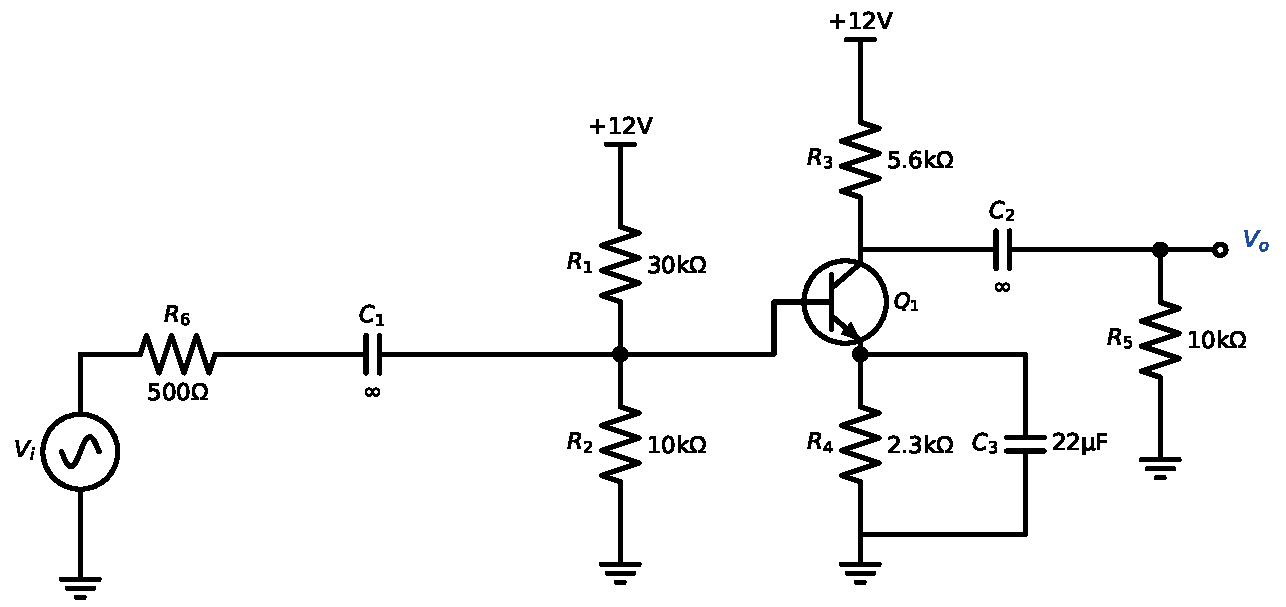
\includegraphics[width=0.9\linewidth,height=6cm,keepaspectratio]{p06_circuit}\end{center}
\solstep{1}{DC currents and small-signal parameters}The DC collector currents are given: $I_{C1} = 1\,\mathrm{m}\mathrm{A}$. For AC every DC supply is ground and every ``$\infty$'' capacitor is a short (tool T3). Small-signal emitter resistances (tool T3):\begin{align*}
r_{e1} &= \frac{V_T}{I_{C1}} = \frac{25\,\mathrm{mV}}{1\,\mathrm{m}\mathrm{A}} = 25\,\Omega
\end{align*}

\solstep{2}{Input resistance of each stage}Input resistance of every stage, from the last stage back to the first (each one loads the stage before it; tool T4):\begin{align*}
R_{i1} &= Z_{base,1} = (\beta+1)(r_{e1} + R_{4} \parallel \frac{1}{sC_{3}}) = \dfrac{2520\,s + 4.64\times 10^{6}}{s + 19.8}
\end{align*}

\solstep{3}{Gain along the signal path}Multiply the node-to-node gains along the signal path (tool T4):\[
H(s) = \frac{v_{b1}}{v_i}\cdot\frac{v_{c1}}{v_{b1}}
\]
\begin{align*}
\frac{v_{b1}}{v_i} &= \frac{R_{1} \parallel R_{2} \parallel R_{i1}}{R_{6} + R_{1} \parallel R_{2} \parallel R_{i1}} = \dfrac{0.791\,s + 1450}{s + 1550} \\
\frac{v_{c1}}{v_{b1}} &= -\alpha\frac{Z_{C1}}{r_{e1} + Z_{E1}},\quad Z_{C1} = R_{3} \parallel R_{5},\ Z_{E1} = R_{4} \parallel \frac{1}{sC_{3}}\ \Rightarrow\ \dfrac{-142\,s - 2810}{s + 1840}
\end{align*}

\solstep{4}{Transfer function}Multiply and simplify:\[
H(s) = \dfrac{-112\,s - 2220}{s + 1550}
\]

\solstep{5}{Standard (Bode-ready) form}Find the roots. Every root $s=-p$ of the denominator is a \emph{pole}, every root $s=-z$ of the numerator is a \emph{zero}; $|p|$ and $|z|$ are the corner frequencies (rad/s).
\begin{itemize}[leftmargin=*,itemsep=2pt]
\item Numerator: $-112\,s - 2220$; divide by the leading coefficient $-112$ (this does not move the roots): $s + 19.8$; $s + 19.8 = 0 \Rightarrow s = -19.8$.
\item Denominator: $s + 1550$; $s + 1550 = 0 \Rightarrow s = -1550$.
\end{itemize}

Factored form (leading coefficient in front):
\[
H(s) = -112\,\dfrac{(s+19.8)}{(s+1550)}
\]

Bode-ready form: rewrite every $(s+p) = p\left(1+\frac{s}{p}\right)$ and $(s+z) = z\left(1+\frac{s}{z}\right)$, and collect all constants into $K$. Then every factor except $K$ is $\approx 1$ inside the pass-band:
\[
H(s) = -1.43\,\left(1+\dfrac{s}{2\pi\cdot 3.15}\right)\,\dfrac{1}{1+\dfrac{s}{2\pi\cdot 247}},\qquad K = -1.43
\]

\begin{center}\renewcommand{\arraystretch}{1.35}
\begin{tabular}{cccc}
\toprule
type & $\omega_c$ (rad/s) & $f_c=\omega_c/2\pi$ & slope change \\
\midrule
zero & $19.8$ & 3.15 Hz & $+20$ dB/dec \\
pole & $1550$ & 247 Hz & $-20$ dB/dec \\
\bottomrule
\end{tabular}\end{center}

\solstep{6}{Magnitude Bode plot}Below every corner, all factors are $\approx$ constant: $|H| \approx 1.43$ $= 3.11$\,dB (flat, 0 dB/dec). Then, moving right, each pole bends the line down by 20\,dB/dec and each zero bends it up by 20\,dB/dec (tool T6):
\begin{center}\renewcommand{\arraystretch}{1.35}
\begin{tabular}{lcl}
\toprule
frequency range & slope & asymptote level \\
\midrule
$f<$ 3.15 Hz & $0$ dB/dec (flat) & 3.11 dB at end \\
3.15 Hz -- 247 Hz & $+20$ dB/dec & 3.11 dB at start, 41 dB at end \\
$f>$ 247 Hz & $0$ dB/dec (flat) & 41 dB at start \\
\bottomrule
\end{tabular}\end{center}

\begin{center}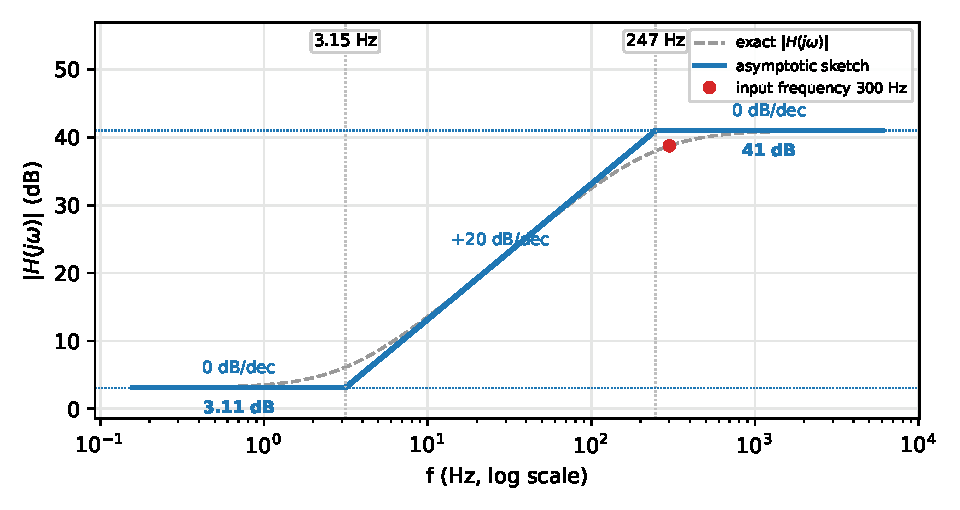
\includegraphics[width=0.78\linewidth,height=6.5cm,keepaspectratio]{p06_bode}\end{center}

{\small Blue: the straight-line sketch you are expected to draw. Dashed grey: the exact curve (about 3\,dB below the corner of an isolated pole). Red dot: the input frequency of Step 7.}
\solstep{7}{Steady-state output}The input is $V_i(t) = 0.005\sin\left(2\pi\cdot 300\,t\right)$, so $\omega_{in} = 2\pi\cdot 300 = 1880$\,rad/s. Put $s=j\omega_{in}$ in each factor (tool T5): magnitudes multiply, angles add.
{\small Rules: $\left|\frac{s}{s+p}\right| = \frac{\omega}{\sqrt{\omega^2+p^2}}$, $\angle = \frac{\pi}{2}-\tan^{-1}\frac{\omega}{p}$;\quad $\left|\frac{1}{1+s/p}\right| = \frac{1}{\sqrt{1+(\omega/p)^2}}$, $\angle = -\tan^{-1}\frac{\omega}{p}$;\quad $\left|1+\frac{s}{z}\right| = \sqrt{1+(\omega/z)^2}$, $\angle = \tan^{-1}\frac{\omega}{z}$;\quad a negative $K$ adds $-\pi$.}
\begin{center}\renewcommand{\arraystretch}{1.35}
\begin{tabular}{ccc}
\toprule
factor & magnitude & angle (rad) \\
\midrule
$-1.43$ & $1.43$ & $-3.14$ \\
$\rule[-1.1em]{0pt}{2.8em}\left(1+\dfrac{s}{2\pi\cdot 3.15}\right)$ & $95.38$ & $1.56$ \\
$\rule[-1.7em]{0pt}{4em}\dfrac{1}{1+\dfrac{s}{2\pi\cdot 247}}$ & $0.6359$ & $-0.882$ \\
\textbf{total} & $\mathbf{86.76}$ (product) & $\mathbf{-2.46}$ (sum) \\
\bottomrule
\end{tabular}\end{center}

\begin{align*}
|H(j\omega_{in})| &= 86.8, \qquad \angle H(j\omega_{in}) = -2.46\ \mathrm{rad} \\
v_{o,ac}(t) &= 86.8\times 0.005\,\sin\left(2\pi\cdot 300\,t - 2.46\right) = 0.434\,\sin\left(2\pi\cdot 300\,t - 2.46\right)
\end{align*}

\[
\boxed{V_o(t) = 0.434\,\sin\left(2\pi\cdot 300\,t - 2.46\right)\ \mathrm{V}}
\]

\begin{ansbox}
$H(s) = -1.43\,\left(1+\dfrac{s}{2\pi\cdot 3.15}\right)\,\dfrac{1}{1+\dfrac{s}{2\pi\cdot 247}}$\quad (corners: 3.15 Hz, 247 Hz)\\[4pt]
$V_o(t) = 0.434\,\sin\left(2\pi\cdot 300\,t - 2.46\right)\ \mathrm{V}$
\end{ansbox}

\newpage
\subsection*{Solution 4D.7 \hfill Medium}
\begin{center}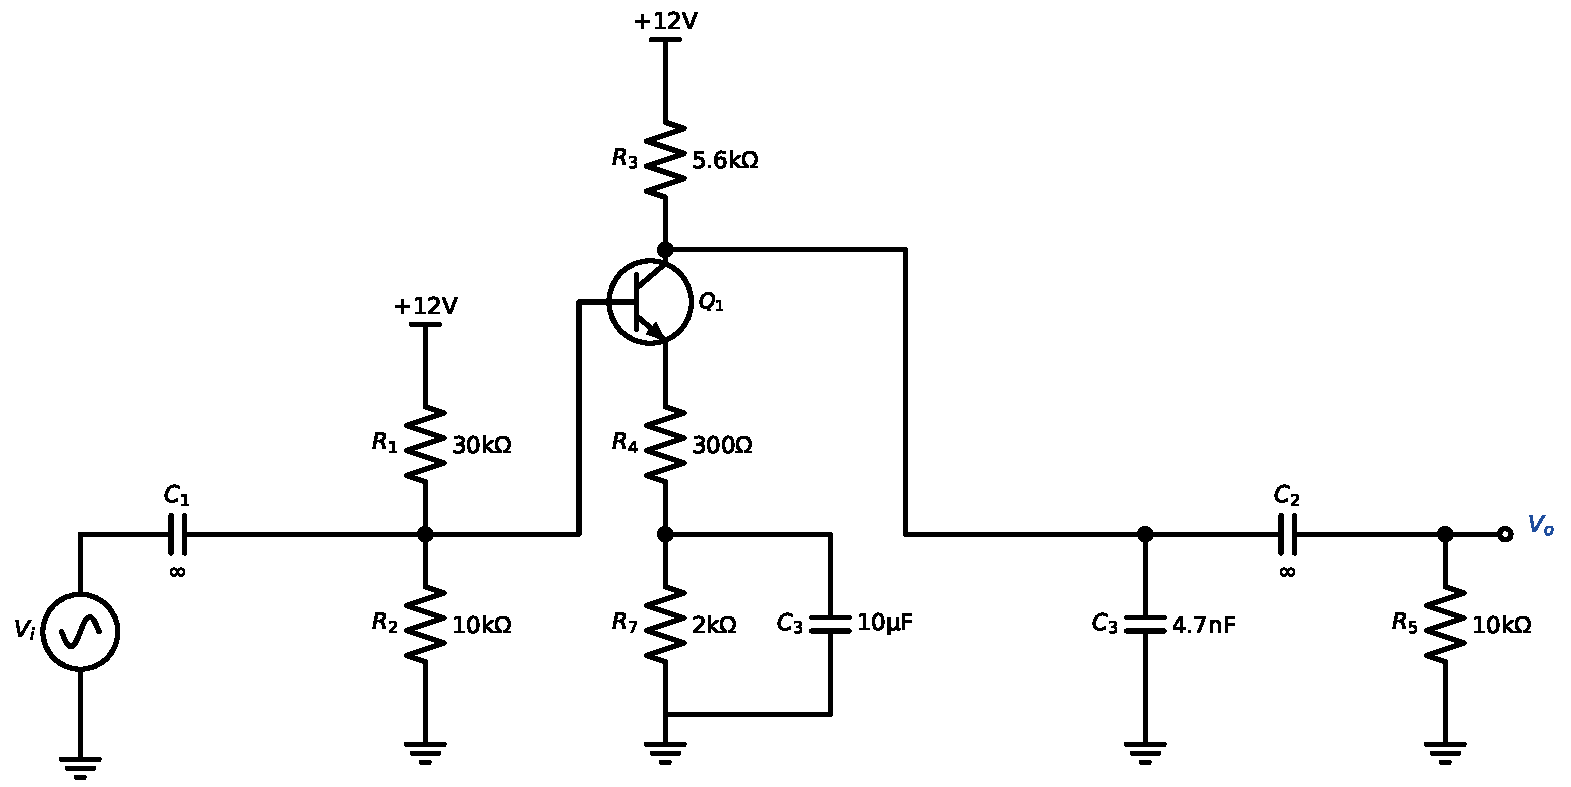
\includegraphics[width=0.9\linewidth,height=6cm,keepaspectratio]{p07_circuit}\end{center}
\solstep{1}{DC currents and small-signal parameters}The DC collector currents are given: $I_{C1} = 1\,\mathrm{m}\mathrm{A}$. For AC every DC supply is ground and every ``$\infty$'' capacitor is a short (tool T3). Small-signal emitter resistances (tool T3):\begin{align*}
r_{e1} &= \frac{V_T}{I_{C1}} = \frac{25\,\mathrm{mV}}{1\,\mathrm{m}\mathrm{A}} = 25\,\Omega
\end{align*}

\solstep{2}{Input resistance of each stage}Input resistance of every stage, from the last stage back to the first (each one loads the stage before it; tool T4):\begin{align*}
R_{i1} &= Z_{base,1} = (\beta+1)(r_{e1} + R_{4} + \left(R_{7} \parallel \frac{1}{sC_{3}}\right)) = \dfrac{32800\,s + 1.17\times 10^{7}}{s + 50}
\end{align*}

\solstep{3}{Gain along the signal path}Multiply the node-to-node gains along the signal path (tool T4):\[
H(s) = \frac{v_{c1}}{v_{b1}}
\]
\begin{align*}
\frac{v_{c1}}{v_{b1}} &= -\alpha\frac{Z_{C1}}{r_{e1} + Z_{E1}},\quad Z_{C1} = R_{3} \parallel \frac{1}{sC_{3}} \parallel R_{5},\ Z_{E1} = R_{4} + \left(R_{7} \parallel \frac{1}{sC_{3}}\right)\ \Rightarrow\ \dfrac{-6.48\times 10^{5}\,s - 3.24\times 10^{7}}{s^{2} + 59600\,s + 2.12\times 10^{7}}
\end{align*}

\solstep{4}{Transfer function}Multiply and simplify:\[
H(s) = \dfrac{-6.48\times 10^{5}\,s - 3.24\times 10^{7}}{s^{2} + 59600\,s + 2.12\times 10^{7}}
\]

\solstep{5}{Standard (Bode-ready) form}Find the roots. Every root $s=-p$ of the denominator is a \emph{pole}, every root $s=-z$ of the numerator is a \emph{zero}; $|p|$ and $|z|$ are the corner frequencies (rad/s).
\begin{itemize}[leftmargin=*,itemsep=2pt]
\item Numerator: $-6.48\times 10^{5}\,s - 3.24\times 10^{7}$; divide by the leading coefficient $-6.48\times 10^{5}$ (this does not move the roots): $s + 50$; $s + 50 = 0 \Rightarrow s = -50$.
\item Denominator: $s^{2} + 59600\,s + 2.12\times 10^{7}$; quadratic formula:\[
s = \frac{-59600 \pm \sqrt{(59600)^2 - 4(2.12\times 10^{7})}}{2} = \frac{-59600 \pm 58900}{2} \Rightarrow s = -358,\ -59300
\]

\end{itemize}

Factored form (leading coefficient in front):
\[
H(s) = -6.48\times 10^{5}\,\dfrac{(s+50)}{(s+358)(s+59300)}
\]

Bode-ready form: rewrite every $(s+p) = p\left(1+\frac{s}{p}\right)$ and $(s+z) = z\left(1+\frac{s}{z}\right)$, and collect all constants into $K$. Then every factor except $K$ is $\approx 1$ inside the pass-band:
\[
H(s) = -1.53\,\left(1+\dfrac{s}{2\pi\cdot 7.96}\right)\,\dfrac{1}{1+\dfrac{s}{2\pi\cdot 56.9}}\,\dfrac{1}{1+\dfrac{s}{2\pi\cdot 9.43\mathrm{k}}},\qquad K = -1.53
\]

\begin{center}\renewcommand{\arraystretch}{1.35}
\begin{tabular}{cccc}
\toprule
type & $\omega_c$ (rad/s) & $f_c=\omega_c/2\pi$ & slope change \\
\midrule
zero & $50$ & 7.96 Hz & $+20$ dB/dec \\
pole & $358$ & 56.9 Hz & $-20$ dB/dec \\
pole & $59300$ & 9.43 kHz & $-20$ dB/dec \\
\bottomrule
\end{tabular}\end{center}

\solstep{6}{Magnitude Bode plot}Below every corner, all factors are $\approx$ constant: $|H| \approx 1.53$ $= 3.69$\,dB (flat, 0 dB/dec). Then, moving right, each pole bends the line down by 20\,dB/dec and each zero bends it up by 20\,dB/dec (tool T6):
\begin{center}\renewcommand{\arraystretch}{1.35}
\begin{tabular}{lcl}
\toprule
frequency range & slope & asymptote level \\
\midrule
$f<$ 7.96 Hz & $0$ dB/dec (flat) & 3.69 dB at end \\
7.96 Hz -- 56.9 Hz & $+20$ dB/dec & 3.69 dB at start, 20.8 dB at end \\
56.9 Hz -- 9.43 kHz & $0$ dB/dec (flat) & 20.8 dB at start, 20.8 dB at end \\
$f>$ 9.43 kHz & $-20$ dB/dec & 20.8 dB at start \\
\bottomrule
\end{tabular}\end{center}

\begin{center}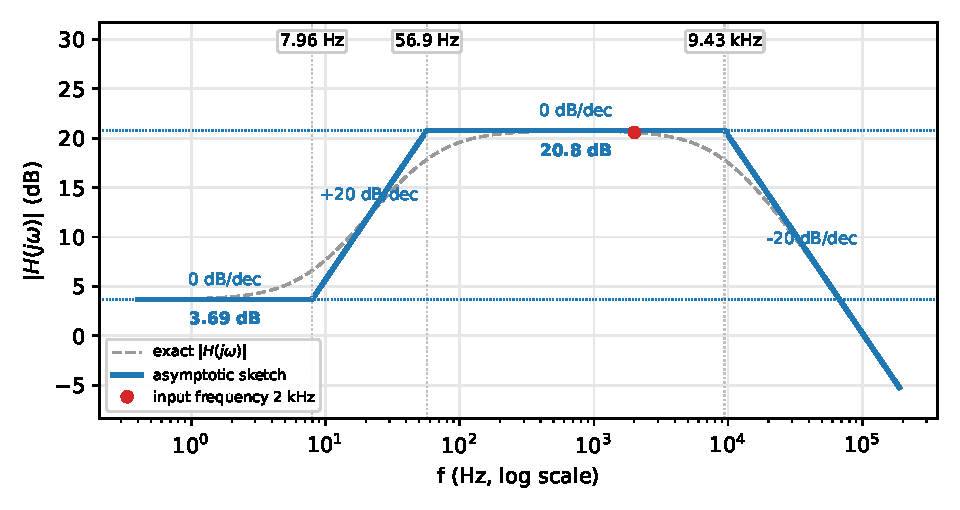
\includegraphics[width=0.78\linewidth,height=6.5cm,keepaspectratio]{p07_bode}\end{center}

{\small Blue: the straight-line sketch you are expected to draw. Dashed grey: the exact curve (about 3\,dB below the corner of an isolated pole). Red dot: the input frequency of Step 7.}
\solstep{7}{Steady-state output}The input is $V_i(t) = 0.01\sin\left(2\pi\cdot 2000\,t\right)$, so $\omega_{in} = 2\pi\cdot 2000 = 12600$\,rad/s. Put $s=j\omega_{in}$ in each factor (tool T5): magnitudes multiply, angles add.
{\small Rules: $\left|\frac{s}{s+p}\right| = \frac{\omega}{\sqrt{\omega^2+p^2}}$, $\angle = \frac{\pi}{2}-\tan^{-1}\frac{\omega}{p}$;\quad $\left|\frac{1}{1+s/p}\right| = \frac{1}{\sqrt{1+(\omega/p)^2}}$, $\angle = -\tan^{-1}\frac{\omega}{p}$;\quad $\left|1+\frac{s}{z}\right| = \sqrt{1+(\omega/z)^2}$, $\angle = \tan^{-1}\frac{\omega}{z}$;\quad a negative $K$ adds $-\pi$.}
\begin{center}\renewcommand{\arraystretch}{1.35}
\begin{tabular}{ccc}
\toprule
factor & magnitude & angle (rad) \\
\midrule
$-1.53$ & $1.529$ & $-3.14$ \\
$\rule[-1.1em]{0pt}{2.8em}\left(1+\dfrac{s}{2\pi\cdot 7.96}\right)$ & $251.3$ & $1.57$ \\
$\rule[-1.7em]{0pt}{4em}\dfrac{1}{1+\dfrac{s}{2\pi\cdot 56.9}}$ & $0.02845$ & $-1.54$ \\
$\rule[-1.7em]{0pt}{4em}\dfrac{1}{1+\dfrac{s}{2\pi\cdot 9.43\mathrm{k}}}$ & $0.9783$ & $-0.209$ \\
\textbf{total} & $\mathbf{10.69}$ (product) & $\mathbf{-3.33}$ (sum) \\
\bottomrule
\end{tabular}\end{center}

\begin{align*}
|H(j\omega_{in})| &= 10.7, \qquad \angle H(j\omega_{in}) = -3.33\ \mathrm{rad} \\
v_{o,ac}(t) &= 10.7\times 0.01\,\sin\left(2\pi\cdot 2000\,t - 3.33\right) = 0.107\,\sin\left(2\pi\cdot 2000\,t - 3.33\right)
\end{align*}

\[
\boxed{V_o(t) = 0.107\,\sin\left(2\pi\cdot 2000\,t - 3.33\right)\ \mathrm{V}}
\]

\begin{ansbox}
$H(s) = -1.53\,\left(1+\dfrac{s}{2\pi\cdot 7.96}\right)\,\dfrac{1}{1+\dfrac{s}{2\pi\cdot 56.9}}\,\dfrac{1}{1+\dfrac{s}{2\pi\cdot 9.43\mathrm{k}}}$\quad (corners: 7.96 Hz, 56.9 Hz, 9.43 kHz)\\[4pt]
$V_o(t) = 0.107\,\sin\left(2\pi\cdot 2000\,t - 3.33\right)\ \mathrm{V}$
\end{ansbox}

\newpage
\subsection*{Solution 4D.8 \hfill Medium}
\begin{center}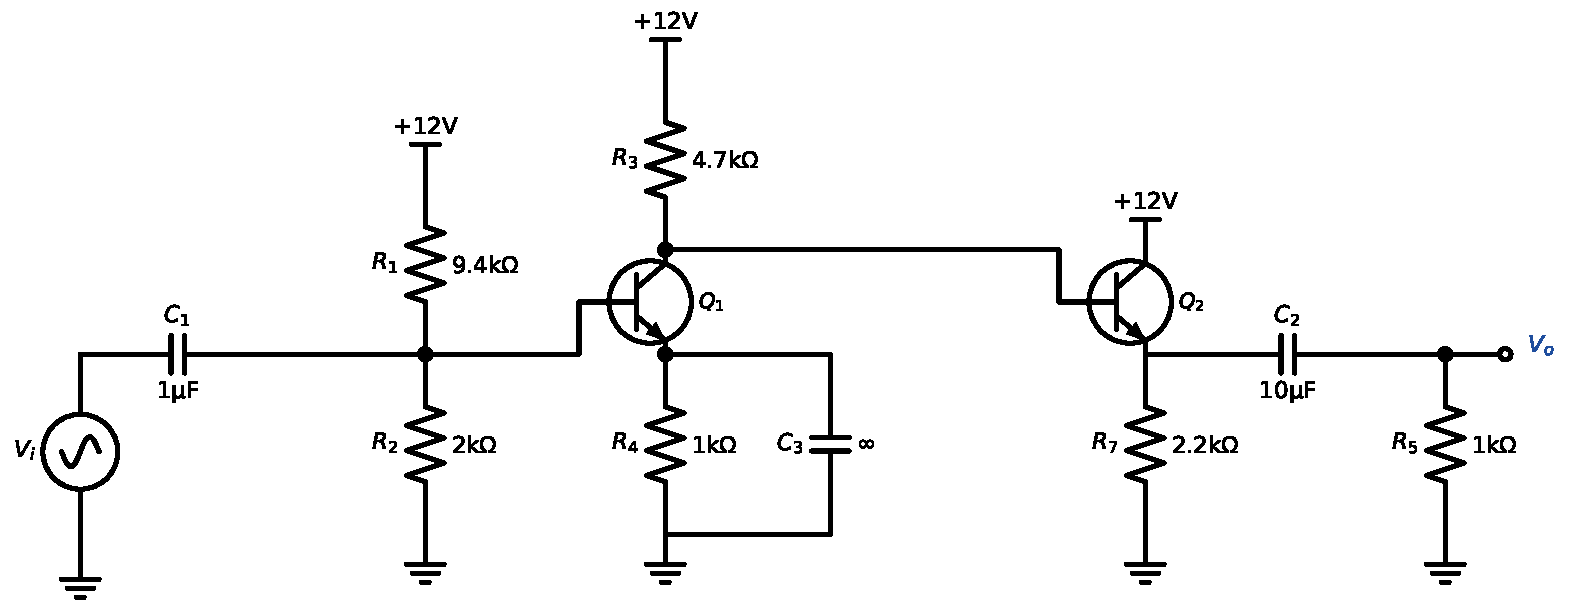
\includegraphics[width=0.9\linewidth,height=6cm,keepaspectratio]{p08_circuit}\end{center}
\solstep{1}{DC currents and small-signal parameters}The DC collector currents are given: $I_{C1} = 1.41\,\mathrm{m}\mathrm{A}$, $I_{C2} = 2.13\,\mathrm{m}\mathrm{A}$. For AC every DC supply is ground and every ``$\infty$'' capacitor is a short (tool T3). Small-signal emitter resistances (tool T3):\begin{align*}
r_{e1} &= \frac{V_T}{I_{C1}} = \frac{25\,\mathrm{mV}}{1.41\,\mathrm{m}\mathrm{A}} = 17.8\,\Omega \\
r_{e2} &= \frac{V_T}{I_{C2}} = \frac{25\,\mathrm{mV}}{2.13\,\mathrm{m}\mathrm{A}} = 11.7\,\Omega
\end{align*}

\solstep{2}{Input resistance of each stage}Input resistance of every stage, from the last stage back to the first (each one loads the stage before it; tool T4):\begin{align*}
R_{i1} &= Z_{base,1} = (\beta+1)(r_{e1} + 0) = 1.8\,\mathrm{k}\Omega \\
R_{i2} &= Z_{base,2} = (\beta+1)(r_{e2} + R_{7} \parallel \left(\frac{1}{sC_{2}} + R_{5}\right)) = \dfrac{70600\,s + 6.98\times 10^{6}}{s + 31.2}
\end{align*}

\solstep{3}{Gain along the signal path}Multiply the node-to-node gains along the signal path (tool T4):\[
H(s) = \frac{v_{b1}}{v_i}\cdot\frac{v_{c1}}{v_{b1}}\cdot\frac{v_{e2}}{v_{b2}}\cdot\frac{v_o}{v_{e2}}
\]
\begin{align*}
\frac{v_{b1}}{v_i} &= \frac{R_{1} \parallel R_{2} \parallel R_{i1}}{\frac{1}{sC_{1}} + R_{1} \parallel R_{2} \parallel R_{i1}} = \dfrac{s}{s + 1160} \\
\frac{v_{c1}}{v_{b1}} &= -\alpha\frac{Z_{C1}}{r_{e1} + Z_{E1}},\quad Z_{C1} = R_{3} \parallel R_{i2},\ Z_{E1} = 0\ \Rightarrow\ \dfrac{-245\,s - 24200}{s + 94.6} \\
\frac{v_{e2}}{v_{b2}} &= \frac{Z_{E2}}{r_{e2} + Z_{E2}},\quad Z_{E2} = R_{7} \parallel \left(\frac{1}{sC_{2}} + R_{5}\right)\ \Rightarrow\ \dfrac{0.983\,s + 98.3}{s + 98.8} \\
\frac{v_o}{v_{e2}} &= \frac{R_{5}}{\frac{1}{sC_{2}} + R_{5}} = \dfrac{s}{s + 100}
\end{align*}

\solstep{4}{Transfer function}Multiply and simplify:\[
H(s) = \dfrac{-241\,s^{2}}{s^{2} + 1260\,s + 1.1\times 10^{5}}
\]

\solstep{5}{Standard (Bode-ready) form}Find the roots. Every root $s=-p$ of the denominator is a \emph{pole}, every root $s=-z$ of the numerator is a \emph{zero}; $|p|$ and $|z|$ are the corner frequencies (rad/s).
\begin{itemize}[leftmargin=*,itemsep=2pt]
\item Numerator: it has the factor $s^2$ $\Rightarrow$ 2 zeros at $s=0$.
\item Denominator: $s^{2} + 1260\,s + 1.1\times 10^{5}$; quadratic formula:\[
s = \frac{-1260 \pm \sqrt{(1260)^2 - 4(1.1\times 10^{5})}}{2} = \frac{-1260 \pm 1070}{2} \Rightarrow s = -94.6,\ -1160
\]

\end{itemize}

Factored form (leading coefficient in front):
\[
H(s) = -241\,\dfrac{s^{2}}{(s+94.6)(s+1160)}
\]

Bode-ready form: rewrite every $(s+p) = p\left(1+\frac{s}{p}\right)$ and $(s+z) = z\left(1+\frac{s}{z}\right)$, and collect all constants into $K$. Each $s$ in the numerator is paired with one of the \emph{lowest} poles as $\frac{s}{s+p}$ (that factor is $\approx 1$ above $p$). Then every factor except $K$ is $\approx 1$ inside the pass-band:
\[
H(s) = -241\,\dfrac{s}{s+2\pi\cdot 15.1}\,\dfrac{s}{s+2\pi\cdot 185},\qquad K = -241
\]

\begin{center}\renewcommand{\arraystretch}{1.35}
\begin{tabular}{cccc}
\toprule
type & $\omega_c$ (rad/s) & $f_c=\omega_c/2\pi$ & slope change \\
\midrule
pole & $94.6$ & 15.1 Hz & $-20$ dB/dec \\
pole & $1160$ & 185 Hz & $-20$ dB/dec \\
\bottomrule
\end{tabular}\end{center}

\solstep{6}{Magnitude Bode plot}Below every corner $|H(s)|\approx 0.00219\,s^2$, so the plot starts with a slope of $+40$\,dB/dec. Then, moving right, each pole bends the line down by 20\,dB/dec and each zero bends it up by 20\,dB/dec (tool T6):
\begin{center}\renewcommand{\arraystretch}{1.35}
\begin{tabular}{lcl}
\toprule
frequency range & slope & asymptote level \\
\midrule
$f<$ 15.1 Hz & $+40$ dB/dec & 25.9 dB at end \\
15.1 Hz -- 185 Hz & $+20$ dB/dec & 25.9 dB at start, 47.6 dB at end \\
$f>$ 185 Hz & $0$ dB/dec (flat) & 47.6 dB at start \\
\bottomrule
\end{tabular}\end{center}

The flat (pass-band) level is $20\log_{10}|K| = 20\log_{10}241 = 47.6$\,dB.
\begin{center}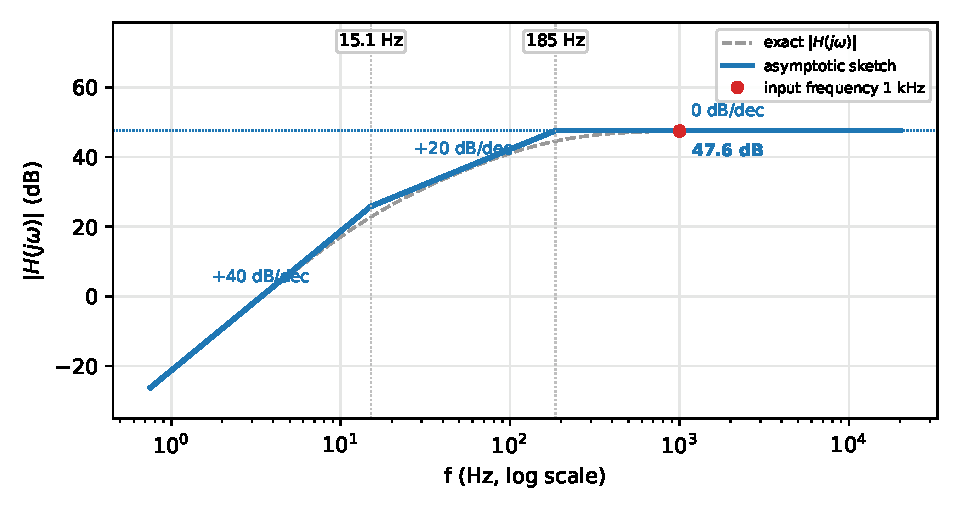
\includegraphics[width=0.78\linewidth,height=6.5cm,keepaspectratio]{p08_bode}\end{center}

{\small Blue: the straight-line sketch you are expected to draw. Dashed grey: the exact curve (about 3\,dB below the corner of an isolated pole). Red dot: the input frequency of Step 7.}
\solstep{7}{Steady-state output}The input is $V_i(t) = 0.002\sin\left(2\pi\cdot 1000\,t\right)$, so $\omega_{in} = 2\pi\cdot 1000 = 6280$\,rad/s. Put $s=j\omega_{in}$ in each factor (tool T5): magnitudes multiply, angles add.
{\small Rules: $\left|\frac{s}{s+p}\right| = \frac{\omega}{\sqrt{\omega^2+p^2}}$, $\angle = \frac{\pi}{2}-\tan^{-1}\frac{\omega}{p}$;\quad $\left|\frac{1}{1+s/p}\right| = \frac{1}{\sqrt{1+(\omega/p)^2}}$, $\angle = -\tan^{-1}\frac{\omega}{p}$;\quad $\left|1+\frac{s}{z}\right| = \sqrt{1+(\omega/z)^2}$, $\angle = \tan^{-1}\frac{\omega}{z}$;\quad a negative $K$ adds $-\pi$.}
\begin{center}\renewcommand{\arraystretch}{1.35}
\begin{tabular}{ccc}
\toprule
factor & magnitude & angle (rad) \\
\midrule
$-241$ & $241.1$ & $-3.14$ \\
$\rule[-1.1em]{0pt}{2.8em}\dfrac{s}{s+2\pi\cdot 15.1}$ & $0.9999$ & $0.0151$ \\
$\rule[-1.1em]{0pt}{2.8em}\dfrac{s}{s+2\pi\cdot 185}$ & $0.9833$ & $0.183$ \\
\textbf{total} & $\mathbf{237.1}$ (product) & $\mathbf{-2.94}$ (sum) \\
\bottomrule
\end{tabular}\end{center}

\begin{align*}
|H(j\omega_{in})| &= 237, \qquad \angle H(j\omega_{in}) = -2.94\ \mathrm{rad} \\
v_{o,ac}(t) &= 237\times 0.002\,\sin\left(2\pi\cdot 1000\,t - 2.94\right) = 0.474\,\sin\left(2\pi\cdot 1000\,t - 2.94\right)
\end{align*}

\[
\boxed{V_o(t) = 0.474\,\sin\left(2\pi\cdot 1000\,t - 2.94\right)\ \mathrm{V}}
\]

\begin{ansbox}
$H(s) = -241\,\dfrac{s}{s+2\pi\cdot 15.1}\,\dfrac{s}{s+2\pi\cdot 185}$\quad (corners: 15.1 Hz, 185 Hz)\\[4pt]
$V_o(t) = 0.474\,\sin\left(2\pi\cdot 1000\,t - 2.94\right)\ \mathrm{V}$
\end{ansbox}

\newpage
\subsection*{Solution 4D.9 \hfill Medium}
\begin{center}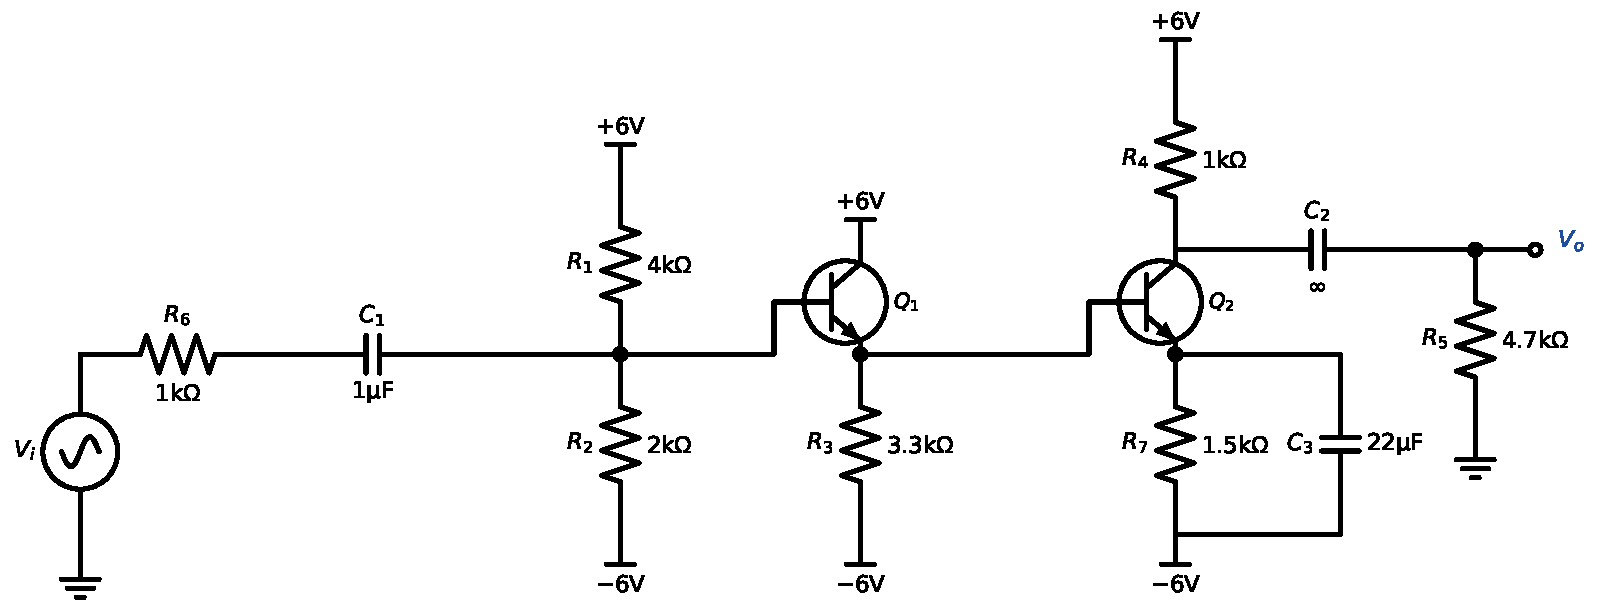
\includegraphics[width=0.9\linewidth,height=6cm,keepaspectratio]{p09_circuit}\end{center}
\solstep{1}{DC currents and small-signal parameters}The DC collector currents are given: $I_{C1} = 1\,\mathrm{m}\mathrm{A}$, $I_{C2} = 1.73\,\mathrm{m}\mathrm{A}$. For AC every DC supply is ground and every ``$\infty$'' capacitor is a short (tool T3). Small-signal emitter resistances (tool T3):\begin{align*}
r_{e1} &= \frac{V_T}{I_{C1}} = \frac{25\,\mathrm{mV}}{1\,\mathrm{m}\mathrm{A}} = 25\,\Omega \\
r_{e2} &= \frac{V_T}{I_{C2}} = \frac{25\,\mathrm{mV}}{1.73\,\mathrm{m}\mathrm{A}} = 14.4\,\Omega
\end{align*}

\solstep{2}{Input resistance of each stage}Input resistance of every stage, from the last stage back to the first (each one loads the stage before it; tool T4):\begin{align*}
R_{i1} &= Z_{base,1} = (\beta+1)(r_{e1} + R_{3} \parallel R_{i2}) = \dfrac{1.05\times 10^{5}\,s + 3.27\times 10^{8}}{s + 995} \\
R_{i2} &= Z_{base,2} = (\beta+1)(r_{e2} + R_{7} \parallel \frac{1}{sC_{3}}) = \dfrac{1460\,s + 4.64\times 10^{6}}{s + 30.3}
\end{align*}

\solstep{3}{Gain along the signal path}Multiply the node-to-node gains along the signal path (tool T4):\[
H(s) = \frac{v_{b1}}{v_i}\cdot\frac{v_{e1}}{v_{b1}}\cdot\frac{v_{c2}}{v_{b2}}
\]
\begin{align*}
\frac{v_{b1}}{v_i} &= \frac{R_{1} \parallel R_{2} \parallel R_{i1}}{R_{6} + \frac{1}{sC_{1}} + R_{1} \parallel R_{2} \parallel R_{i1}} = \dfrac{0.568\,s^{2} + 1780\,s}{s^{2} + 3550\,s + 1.34\times 10^{6}} \\
\frac{v_{e1}}{v_{b1}} &= \frac{Z_{E1}}{r_{e1} + Z_{E1}},\quad Z_{E1} = R_{3} \parallel R_{i2}\ \Rightarrow\ \dfrac{0.976\,s + 3110}{s + 3130} \\
\frac{v_{c2}}{v_{b2}} &= -\alpha\frac{Z_{C2}}{r_{e2} + Z_{E2}},\quad Z_{C2} = R_{4} \parallel R_{5},\ Z_{E2} = R_{7} \parallel \frac{1}{sC_{3}}\ \Rightarrow\ \dfrac{-56.6\,s - 1720}{s + 3180}
\end{align*}

\solstep{4}{Transfer function}Multiply and simplify:\[
H(s) = \dfrac{-31.4\,s^{2} - 951\,s}{s^{2} + 3550\,s + 1.34\times 10^{6}}
\]

\solstep{5}{Standard (Bode-ready) form}Find the roots. Every root $s=-p$ of the denominator is a \emph{pole}, every root $s=-z$ of the numerator is a \emph{zero}; $|p|$ and $|z|$ are the corner frequencies (rad/s).
\begin{itemize}[leftmargin=*,itemsep=2pt]
\item Numerator: it has the factor $s$ $\Rightarrow$ 1 zero at $s=0$.
\item Numerator (after taking out the $s$ factor): $-31.4\,s - 951$; divide by the leading coefficient $-31.4$ (this does not move the roots): $s + 30.3$; $s + 30.3 = 0 \Rightarrow s = -30.3$.
\item Denominator: $s^{2} + 3550\,s + 1.34\times 10^{6}$; quadratic formula:\[
s = \frac{-3550 \pm \sqrt{(3550)^2 - 4(1.34\times 10^{6})}}{2} = \frac{-3550 \pm 2690}{2} \Rightarrow s = -429,\ -3120
\]

\end{itemize}

Factored form (leading coefficient in front):
\[
H(s) = -31.4\,\dfrac{s(s+30.3)}{(s+429)(s+3120)}
\]

Bode-ready form: rewrite every $(s+p) = p\left(1+\frac{s}{p}\right)$ and $(s+z) = z\left(1+\frac{s}{z}\right)$, and collect all constants into $K$. Each $s$ in the numerator is paired with one of the \emph{lowest} poles as $\frac{s}{s+p}$ (that factor is $\approx 1$ above $p$). Then every factor except $K$ is $\approx 1$ inside the pass-band:
\[
H(s) = -0.305\,\dfrac{s}{s+2\pi\cdot 68.3}\,\left(1+\dfrac{s}{2\pi\cdot 4.82}\right)\,\dfrac{1}{1+\dfrac{s}{2\pi\cdot 497}},\qquad K = -0.305
\]

\begin{center}\renewcommand{\arraystretch}{1.35}
\begin{tabular}{cccc}
\toprule
type & $\omega_c$ (rad/s) & $f_c=\omega_c/2\pi$ & slope change \\
\midrule
zero & $30.3$ & 4.82 Hz & $+20$ dB/dec \\
pole & $429$ & 68.3 Hz & $-20$ dB/dec \\
pole & $3120$ & 497 Hz & $-20$ dB/dec \\
\bottomrule
\end{tabular}\end{center}

\solstep{6}{Magnitude Bode plot}Below every corner $|H(s)|\approx 7.1\times 10^{-4}\,s$, so the plot starts with a slope of $+20$\,dB/dec. Then, moving right, each pole bends the line down by 20\,dB/dec and each zero bends it up by 20\,dB/dec (tool T6):
\begin{center}\renewcommand{\arraystretch}{1.35}
\begin{tabular}{lcl}
\toprule
frequency range & slope & asymptote level \\
\midrule
$f<$ 4.82 Hz & $+20$ dB/dec & -33.3 dB at end \\
4.82 Hz -- 68.3 Hz & $+40$ dB/dec & -33.3 dB at start, 12.7 dB at end \\
68.3 Hz -- 497 Hz & $+20$ dB/dec & 12.7 dB at start, 29.9 dB at end \\
$f>$ 497 Hz & $0$ dB/dec (flat) & 29.9 dB at start \\
\bottomrule
\end{tabular}\end{center}

\begin{center}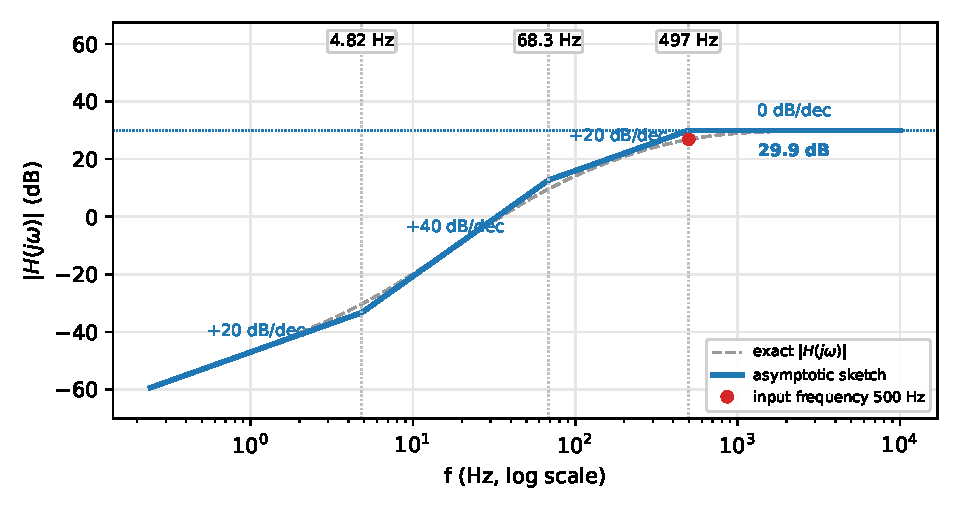
\includegraphics[width=0.78\linewidth,height=6.5cm,keepaspectratio]{p09_bode}\end{center}

{\small Blue: the straight-line sketch you are expected to draw. Dashed grey: the exact curve (about 3\,dB below the corner of an isolated pole). Red dot: the input frequency of Step 7.}
\solstep{7}{Steady-state output}The input is $V_i(t) = 0.005\sin\left(2\pi\cdot 500\,t\right)$, so $\omega_{in} = 2\pi\cdot 500 = 3140$\,rad/s. Put $s=j\omega_{in}$ in each factor (tool T5): magnitudes multiply, angles add.
{\small Rules: $\left|\frac{s}{s+p}\right| = \frac{\omega}{\sqrt{\omega^2+p^2}}$, $\angle = \frac{\pi}{2}-\tan^{-1}\frac{\omega}{p}$;\quad $\left|\frac{1}{1+s/p}\right| = \frac{1}{\sqrt{1+(\omega/p)^2}}$, $\angle = -\tan^{-1}\frac{\omega}{p}$;\quad $\left|1+\frac{s}{z}\right| = \sqrt{1+(\omega/z)^2}$, $\angle = \tan^{-1}\frac{\omega}{z}$;\quad a negative $K$ adds $-\pi$.}
\begin{center}\renewcommand{\arraystretch}{1.35}
\begin{tabular}{ccc}
\toprule
factor & magnitude & angle (rad) \\
\midrule
$-0.305$ & $0.3049$ & $-3.14$ \\
$\rule[-1.1em]{0pt}{2.8em}\dfrac{s}{s+2\pi\cdot 68.3}$ & $0.9908$ & $0.136$ \\
$\rule[-1.1em]{0pt}{2.8em}\left(1+\dfrac{s}{2\pi\cdot 4.82}\right)$ & $103.7$ & $1.56$ \\
$\rule[-1.7em]{0pt}{4em}\dfrac{1}{1+\dfrac{s}{2\pi\cdot 497}}$ & $0.7047$ & $-0.789$ \\
\textbf{total} & $\mathbf{22.07}$ (product) & $\mathbf{-2.23}$ (sum) \\
\bottomrule
\end{tabular}\end{center}

\begin{align*}
|H(j\omega_{in})| &= 22.1, \qquad \angle H(j\omega_{in}) = -2.23\ \mathrm{rad} \\
v_{o,ac}(t) &= 22.1\times 0.005\,\sin\left(2\pi\cdot 500\,t - 2.23\right) = 0.11\,\sin\left(2\pi\cdot 500\,t - 2.23\right)
\end{align*}

\[
\boxed{V_o(t) = 0.11\,\sin\left(2\pi\cdot 500\,t - 2.23\right)\ \mathrm{V}}
\]

\begin{ansbox}
$H(s) = -0.305\,\dfrac{s}{s+2\pi\cdot 68.3}\,\left(1+\dfrac{s}{2\pi\cdot 4.82}\right)\,\dfrac{1}{1+\dfrac{s}{2\pi\cdot 497}}$\quad (corners: 4.82 Hz, 68.3 Hz, 497 Hz)\\[4pt]
$V_o(t) = 0.11\,\sin\left(2\pi\cdot 500\,t - 2.23\right)\ \mathrm{V}$
\end{ansbox}

\newpage
\subsection*{Solution 4D.10 \hfill Medium}
\begin{center}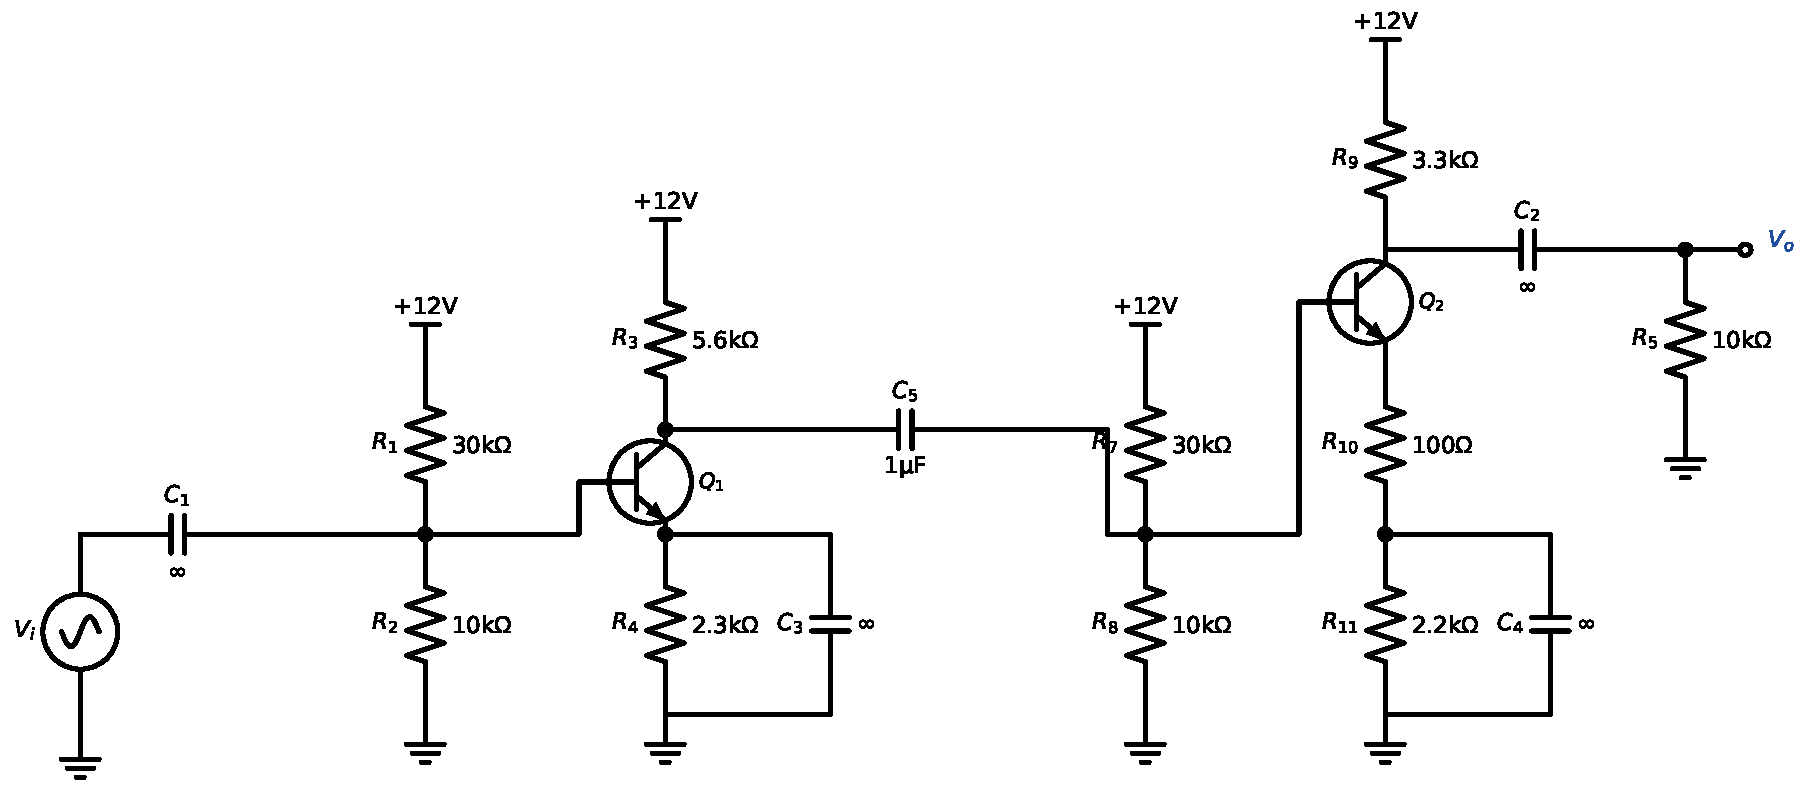
\includegraphics[width=0.9\linewidth,height=6cm,keepaspectratio]{p10_circuit}\end{center}
\solstep{1}{DC currents and small-signal parameters}The DC collector currents are given: $I_{C1} = 1\,\mathrm{m}\mathrm{A}$, $I_{C2} = 1\,\mathrm{m}\mathrm{A}$. For AC every DC supply is ground and every ``$\infty$'' capacitor is a short (tool T3). Small-signal emitter resistances (tool T3):\begin{align*}
r_{e1} &= \frac{V_T}{I_{C1}} = \frac{25\,\mathrm{mV}}{1\,\mathrm{m}\mathrm{A}} = 25\,\Omega \\
r_{e2} &= \frac{V_T}{I_{C2}} = \frac{25\,\mathrm{mV}}{1\,\mathrm{m}\mathrm{A}} = 25\,\Omega
\end{align*}

\solstep{2}{Input resistance of each stage}Input resistance of every stage, from the last stage back to the first (each one loads the stage before it; tool T4):\begin{align*}
R_{i1} &= Z_{base,1} = (\beta+1)(r_{e1} + 0) = 2.52\,\mathrm{k}\Omega \\
R_{i2} &= Z_{base,2} = (\beta+1)(r_{e2} + R_{10}) = 12.6\,\mathrm{k}\Omega
\end{align*}

\solstep{3}{Gain along the signal path}Multiply the node-to-node gains along the signal path (tool T4):\[
H(s) = \frac{v_{c1}}{v_{b1}}\cdot\frac{v_{b2}}{v_{c1}}\cdot\frac{v_{c2}}{v_{b2}}
\]
\begin{align*}
\frac{v_{c1}}{v_{b1}} &= -\alpha\frac{Z_{C1}}{r_{e1} + Z_{E1}},\quad Z_{C1} = R_{3} \parallel \left(\frac{1}{sC_{5}} + \left(R_{7} \parallel R_{8} \parallel R_{i2}\right)\right),\ Z_{E1} = 0\ \Rightarrow\ \dfrac{-101\,s - 21500}{s + 97} \\
\frac{v_{b2}}{v_{c1}} &= \frac{R_{7} \parallel R_{8} \parallel R_{i2}}{\frac{1}{sC_{5}} + R_{7} \parallel R_{8} \parallel R_{i2}} = \dfrac{s}{s + 213} \\
\frac{v_{c2}}{v_{b2}} &= -\alpha\frac{Z_{C2}}{r_{e2} + Z_{E2}},\quad Z_{C2} = R_{9} \parallel R_{5},\ Z_{E2} = R_{10}\ \Rightarrow\ -19.7
\end{align*}

\solstep{4}{Transfer function}Multiply and simplify:\[
H(s) = \dfrac{1990\,s}{s + 97}
\]

\solstep{5}{Standard (Bode-ready) form}Find the roots. Every root $s=-p$ of the denominator is a \emph{pole}, every root $s=-z$ of the numerator is a \emph{zero}; $|p|$ and $|z|$ are the corner frequencies (rad/s).
\begin{itemize}[leftmargin=*,itemsep=2pt]
\item Numerator: it has the factor $s$ $\Rightarrow$ 1 zero at $s=0$.
\item Denominator: $s + 97$; $s + 97 = 0 \Rightarrow s = -97$.
\end{itemize}

Factored form (leading coefficient in front):
\[
H(s) = 1990\,\dfrac{s}{(s+97)}
\]

Bode-ready form: rewrite every $(s+p) = p\left(1+\frac{s}{p}\right)$ and $(s+z) = z\left(1+\frac{s}{z}\right)$, and collect all constants into $K$. Each $s$ in the numerator is paired with one of the \emph{lowest} poles as $\frac{s}{s+p}$ (that factor is $\approx 1$ above $p$). Then every factor except $K$ is $\approx 1$ inside the pass-band:
\[
H(s) = 1990\,\dfrac{s}{s+2\pi\cdot 15.4},\qquad K = 1990
\]

\begin{center}\renewcommand{\arraystretch}{1.35}
\begin{tabular}{cccc}
\toprule
type & $\omega_c$ (rad/s) & $f_c=\omega_c/2\pi$ & slope change \\
\midrule
pole & $97$ & 15.4 Hz & $-20$ dB/dec \\
\bottomrule
\end{tabular}\end{center}

\solstep{6}{Magnitude Bode plot}Below every corner $|H(s)|\approx 20.5\,s$, so the plot starts with a slope of $+20$\,dB/dec. Then, moving right, each pole bends the line down by 20\,dB/dec and each zero bends it up by 20\,dB/dec (tool T6):
\begin{center}\renewcommand{\arraystretch}{1.35}
\begin{tabular}{lcl}
\toprule
frequency range & slope & asymptote level \\
\midrule
$f<$ 15.4 Hz & $+20$ dB/dec & 66 dB at end \\
$f>$ 15.4 Hz & $0$ dB/dec (flat) & 66 dB at start \\
\bottomrule
\end{tabular}\end{center}

The flat (pass-band) level is $20\log_{10}|K| = 20\log_{10}1990 = 66$\,dB.
\begin{center}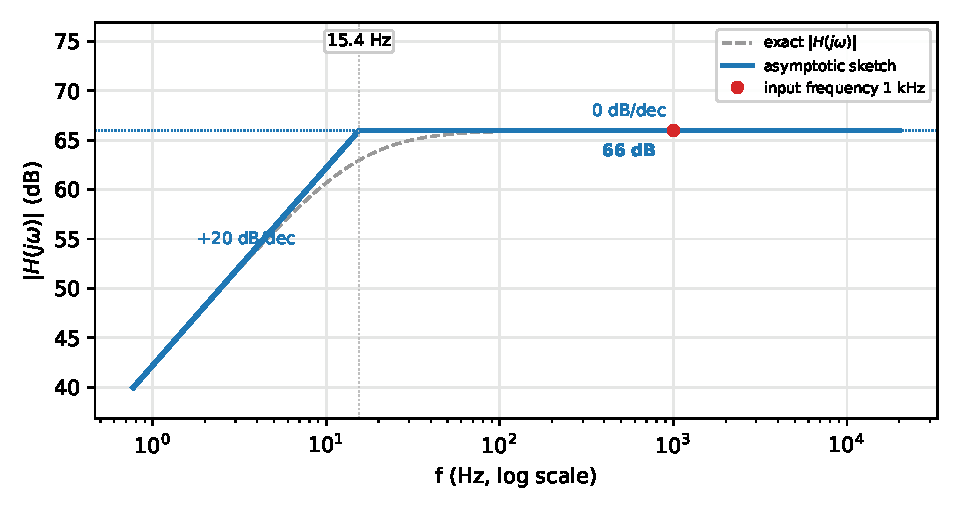
\includegraphics[width=0.78\linewidth,height=6.5cm,keepaspectratio]{p10_bode}\end{center}

{\small Blue: the straight-line sketch you are expected to draw. Dashed grey: the exact curve (about 3\,dB below the corner of an isolated pole). Red dot: the input frequency of Step 7.}
\solstep{7}{Steady-state output}The input is $V_i(t) = 5\times 10^{-4}\sin\left(2\pi\cdot 1000\,t\right)$, so $\omega_{in} = 2\pi\cdot 1000 = 6280$\,rad/s. Put $s=j\omega_{in}$ in each factor (tool T5): magnitudes multiply, angles add.
{\small Rules: $\left|\frac{s}{s+p}\right| = \frac{\omega}{\sqrt{\omega^2+p^2}}$, $\angle = \frac{\pi}{2}-\tan^{-1}\frac{\omega}{p}$;\quad $\left|\frac{1}{1+s/p}\right| = \frac{1}{\sqrt{1+(\omega/p)^2}}$, $\angle = -\tan^{-1}\frac{\omega}{p}$;\quad $\left|1+\frac{s}{z}\right| = \sqrt{1+(\omega/z)^2}$, $\angle = \tan^{-1}\frac{\omega}{z}$;\quad a negative $K$ adds $-\pi$.}
\begin{center}\renewcommand{\arraystretch}{1.35}
\begin{tabular}{ccc}
\toprule
factor & magnitude & angle (rad) \\
\midrule
$1990$ & $1990$ & $0$ \\
$\rule[-1.1em]{0pt}{2.8em}\dfrac{s}{s+2\pi\cdot 15.4}$ & $0.9999$ & $0.0154$ \\
\textbf{total} & $\mathbf{1990}$ (product) & $\mathbf{0.0154}$ (sum) \\
\bottomrule
\end{tabular}\end{center}

\begin{align*}
|H(j\omega_{in})| &= 1990, \qquad \angle H(j\omega_{in}) = 0.0154\ \mathrm{rad} \\
v_{o,ac}(t) &= 1990\times 5\times 10^{-4}\,\sin\left(2\pi\cdot 1000\,t + 0.0154\right) = 0.995\,\sin\left(2\pi\cdot 1000\,t + 0.0154\right)
\end{align*}

\[
\boxed{V_o(t) = 0.995\,\sin\left(2\pi\cdot 1000\,t + 0.0154\right)\ \mathrm{V}}
\]

\begin{ansbox}
$H(s) = 1990\,\dfrac{s}{s+2\pi\cdot 15.4}$\quad (corners: 15.4 Hz)\\[4pt]
$V_o(t) = 0.995\,\sin\left(2\pi\cdot 1000\,t + 0.0154\right)\ \mathrm{V}$
\end{ansbox}

\newpage
\subsection*{Solution 4D.11 \hfill Medium}
\begin{center}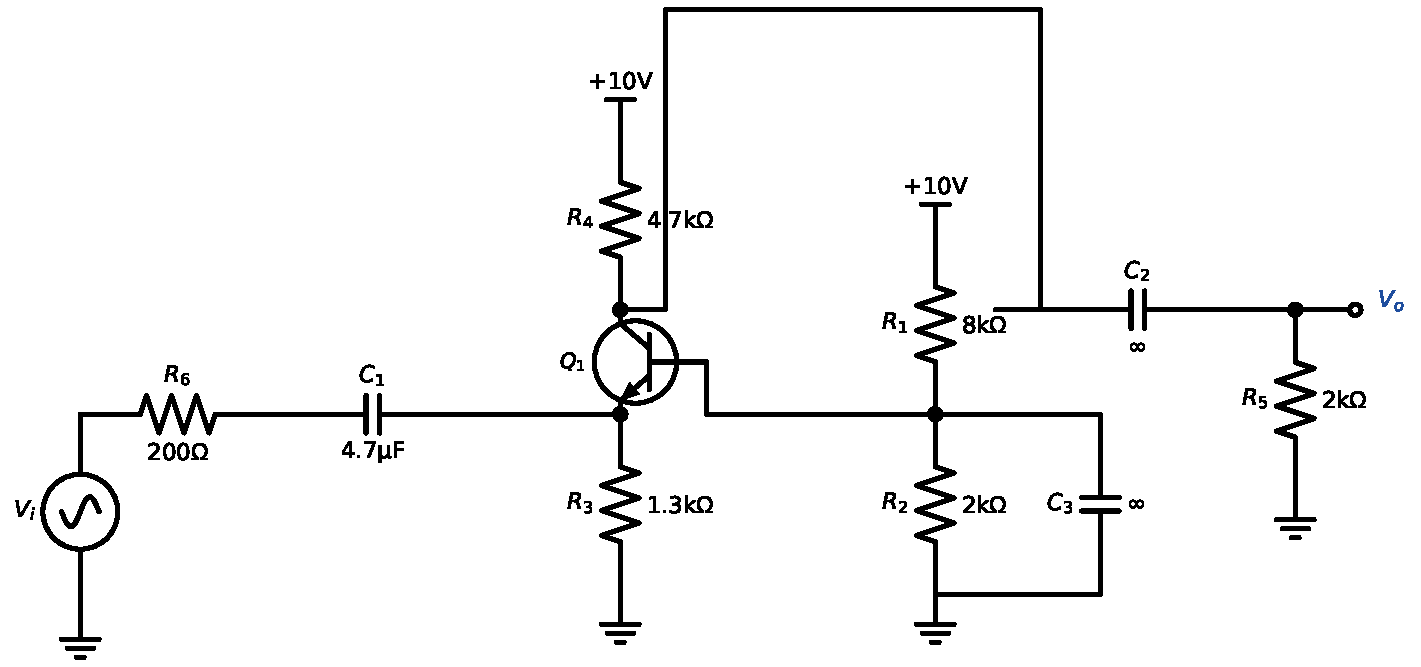
\includegraphics[width=0.9\linewidth,height=6cm,keepaspectratio]{p11_circuit}\end{center}
\solstep{1}{DC currents and small-signal parameters}The DC collector currents are given: $I_{C1} = 1\,\mathrm{m}\mathrm{A}$. For AC every DC supply is ground and every ``$\infty$'' capacitor is a short (tool T3). Small-signal emitter resistances (tool T3):\begin{align*}
r_{e1} &= \frac{V_T}{I_{C1}} = \frac{25\,\mathrm{mV}}{1\,\mathrm{m}\mathrm{A}} = 25\,\Omega
\end{align*}

\solstep{2}{Input resistance of each stage}Input resistance of every stage, from the last stage back to the first (each one loads the stage before it; tool T4):\begin{align*}
R_{i1} &= Z_{emitter,1} = r_{e1} + \frac{0}{\beta+1} = 25\,\Omega
\end{align*}

\solstep{3}{Gain along the signal path}Multiply the node-to-node gains along the signal path (tool T4):\[
H(s) = \frac{v_{e1}}{v_i}\cdot\frac{v_{c1}}{v_{e1}}
\]
\begin{align*}
\frac{v_{e1}}{v_i} &= \frac{R_{3} \parallel R_{i1}}{R_{6} + \frac{1}{sC_{1}} + R_{3} \parallel R_{i1}} = \dfrac{0.109\,s}{s + 948} \\
\frac{v_{c1}}{v_{e1}} &= \alpha\frac{Z_{C1}}{Z_{emitter,1}},\quad Z_{C1} = R_{4} \parallel R_{5}\ \Rightarrow\ 55.6
\end{align*}

\solstep{4}{Transfer function}Multiply and simplify:\[
H(s) = \dfrac{6.07\,s}{s + 948}
\]

\solstep{5}{Standard (Bode-ready) form}Find the roots. Every root $s=-p$ of the denominator is a \emph{pole}, every root $s=-z$ of the numerator is a \emph{zero}; $|p|$ and $|z|$ are the corner frequencies (rad/s).
\begin{itemize}[leftmargin=*,itemsep=2pt]
\item Numerator: it has the factor $s$ $\Rightarrow$ 1 zero at $s=0$.
\item Denominator: $s + 948$; $s + 948 = 0 \Rightarrow s = -948$.
\end{itemize}

Factored form (leading coefficient in front):
\[
H(s) = 6.07\,\dfrac{s}{(s+948)}
\]

Bode-ready form: rewrite every $(s+p) = p\left(1+\frac{s}{p}\right)$ and $(s+z) = z\left(1+\frac{s}{z}\right)$, and collect all constants into $K$. Each $s$ in the numerator is paired with one of the \emph{lowest} poles as $\frac{s}{s+p}$ (that factor is $\approx 1$ above $p$). Then every factor except $K$ is $\approx 1$ inside the pass-band:
\[
H(s) = 6.07\,\dfrac{s}{s+2\pi\cdot 151},\qquad K = 6.07
\]

\begin{center}\renewcommand{\arraystretch}{1.35}
\begin{tabular}{cccc}
\toprule
type & $\omega_c$ (rad/s) & $f_c=\omega_c/2\pi$ & slope change \\
\midrule
pole & $948$ & 151 Hz & $-20$ dB/dec \\
\bottomrule
\end{tabular}\end{center}

\solstep{6}{Magnitude Bode plot}Below every corner $|H(s)|\approx 0.00641\,s$, so the plot starts with a slope of $+20$\,dB/dec. Then, moving right, each pole bends the line down by 20\,dB/dec and each zero bends it up by 20\,dB/dec (tool T6):
\begin{center}\renewcommand{\arraystretch}{1.35}
\begin{tabular}{lcl}
\toprule
frequency range & slope & asymptote level \\
\midrule
$f<$ 151 Hz & $+20$ dB/dec & 15.7 dB at end \\
$f>$ 151 Hz & $0$ dB/dec (flat) & 15.7 dB at start \\
\bottomrule
\end{tabular}\end{center}

The flat (pass-band) level is $20\log_{10}|K| = 20\log_{10}6.07 = 15.7$\,dB.
\begin{center}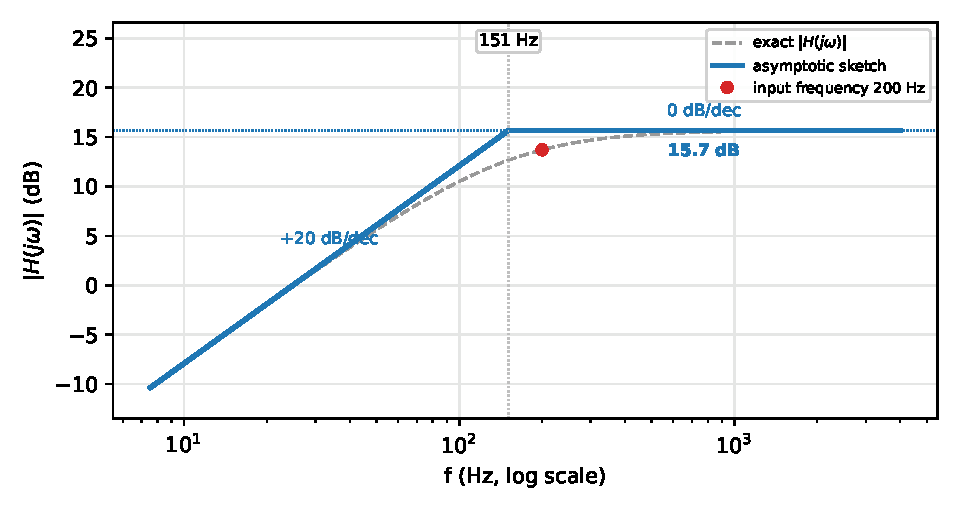
\includegraphics[width=0.78\linewidth,height=6.5cm,keepaspectratio]{p11_bode}\end{center}

{\small Blue: the straight-line sketch you are expected to draw. Dashed grey: the exact curve (about 3\,dB below the corner of an isolated pole). Red dot: the input frequency of Step 7.}
\solstep{7}{Steady-state output}The input is $V_i(t) = 0.02\sin\left(2\pi\cdot 200\,t\right)$, so $\omega_{in} = 2\pi\cdot 200 = 1260$\,rad/s. Put $s=j\omega_{in}$ in each factor (tool T5): magnitudes multiply, angles add.
{\small Rules: $\left|\frac{s}{s+p}\right| = \frac{\omega}{\sqrt{\omega^2+p^2}}$, $\angle = \frac{\pi}{2}-\tan^{-1}\frac{\omega}{p}$;\quad $\left|\frac{1}{1+s/p}\right| = \frac{1}{\sqrt{1+(\omega/p)^2}}$, $\angle = -\tan^{-1}\frac{\omega}{p}$;\quad $\left|1+\frac{s}{z}\right| = \sqrt{1+(\omega/z)^2}$, $\angle = \tan^{-1}\frac{\omega}{z}$;\quad a negative $K$ adds $-\pi$.}
\begin{center}\renewcommand{\arraystretch}{1.35}
\begin{tabular}{ccc}
\toprule
factor & magnitude & angle (rad) \\
\midrule
$6.07$ & $6.07$ & $0$ \\
$\rule[-1.1em]{0pt}{2.8em}\dfrac{s}{s+2\pi\cdot 151}$ & $0.7984$ & $0.646$ \\
\textbf{total} & $\mathbf{4.846}$ (product) & $\mathbf{0.646}$ (sum) \\
\bottomrule
\end{tabular}\end{center}

\begin{align*}
|H(j\omega_{in})| &= 4.85, \qquad \angle H(j\omega_{in}) = 0.646\ \mathrm{rad} \\
v_{o,ac}(t) &= 4.85\times 0.02\,\sin\left(2\pi\cdot 200\,t + 0.646\right) = 0.0969\,\sin\left(2\pi\cdot 200\,t + 0.646\right)
\end{align*}

\[
\boxed{V_o(t) = 0.0969\,\sin\left(2\pi\cdot 200\,t + 0.646\right)\ \mathrm{V}}
\]

\begin{ansbox}
$H(s) = 6.07\,\dfrac{s}{s+2\pi\cdot 151}$\quad (corners: 151 Hz)\\[4pt]
$V_o(t) = 0.0969\,\sin\left(2\pi\cdot 200\,t + 0.646\right)\ \mathrm{V}$
\end{ansbox}

\newpage
\subsection*{Solution 4D.12 \hfill Medium}
\begin{center}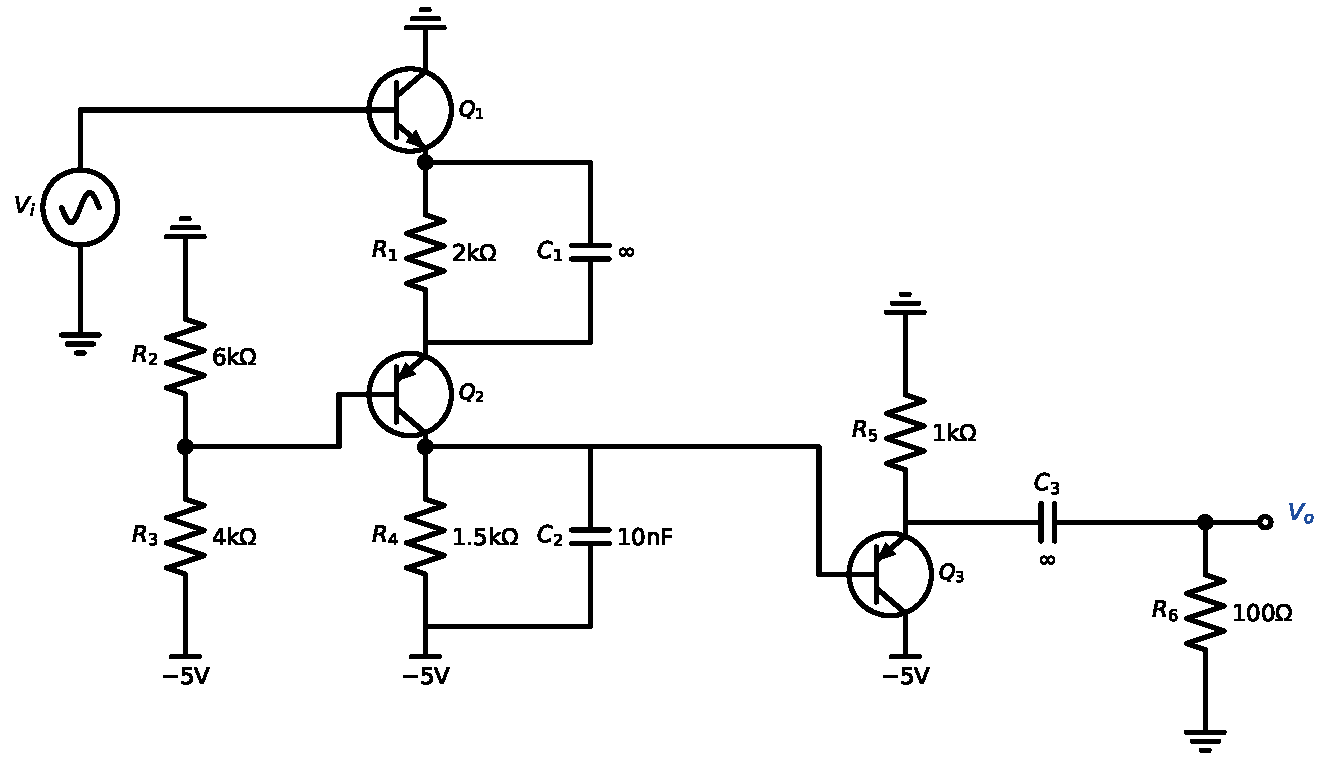
\includegraphics[width=0.9\linewidth,height=6cm,keepaspectratio]{p12_circuit}\end{center}
\solstep{1}{DC currents and small-signal parameters}The DC collector currents are given: $I_{C1} = 800\,\mu \mathrm{A}$, $I_{C2} = 800\,\mu \mathrm{A}$, $I_{C3} = 3.1\,\mathrm{m}\mathrm{A}$. For AC every DC supply is ground and every ``$\infty$'' capacitor is a short (tool T3). Small-signal emitter resistances (tool T3):\begin{align*}
r_{e1} &= \frac{V_T}{I_{C1}} = \frac{25\,\mathrm{mV}}{800\,\mu \mathrm{A}} = 31.2\,\Omega \\
r_{e2} &= \frac{V_T}{I_{C2}} = \frac{25\,\mathrm{mV}}{800\,\mu \mathrm{A}} = 31.2\,\Omega \\
r_{e3} &= \frac{V_T}{I_{C3}} = \frac{25\,\mathrm{mV}}{3.1\,\mathrm{m}\mathrm{A}} = 8.06\,\Omega
\end{align*}

\solstep{2}{Input resistance of each stage}Input resistance of every stage, from the last stage back to the first (each one loads the stage before it; tool T4):\begin{align*}
R_{i1} &= Z_{base,1} = (\beta+1)(r_{e1} + R_{i2}) = 8.71\,\mathrm{k}\Omega \\
R_{i2} &= Z_{emitter,2} = r_{e2} + \frac{R_{2} \parallel R_{3}}{\beta+1} = 55\,\Omega \\
R_{i3} &= Z_{base,3} = (\beta+1)(r_{e3} + R_{5} \parallel R_{6}) = 10\,\mathrm{k}\Omega
\end{align*}

\solstep{3}{Gain along the signal path}Multiply the node-to-node gains along the signal path (tool T4):\[
H(s) = \frac{v_{e1}}{v_{b1}}\cdot\frac{v_{c2}}{v_{e2}}\cdot\frac{v_{e3}}{v_{b3}}
\]
\begin{align*}
\frac{v_{e1}}{v_{b1}} &= \frac{Z_{E1}}{r_{e1} + Z_{E1}},\quad Z_{E1} = R_{i2}\ \Rightarrow\ 0.638 \\
\frac{v_{c2}}{v_{e2}} &= \alpha\frac{Z_{C2}}{Z_{emitter,2}},\quad Z_{C2} = R_{4} \parallel \frac{1}{sC_{2}} \parallel R_{i3}\ \Rightarrow\ \dfrac{1.8\times 10^{6}}{s + 76700} \\
\frac{v_{e3}}{v_{b3}} &= \frac{Z_{E3}}{r_{e3} + Z_{E3}},\quad Z_{E3} = R_{5} \parallel R_{6}\ \Rightarrow\ 0.919
\end{align*}

\solstep{4}{Transfer function}Multiply and simplify:\[
H(s) = \dfrac{1.05\times 10^{6}}{s + 76700}
\]

\solstep{5}{Standard (Bode-ready) form}Find the roots. Every root $s=-p$ of the denominator is a \emph{pole}, every root $s=-z$ of the numerator is a \emph{zero}; $|p|$ and $|z|$ are the corner frequencies (rad/s).
\begin{itemize}[leftmargin=*,itemsep=2pt]
\item Denominator: $s + 76700$; $s + 76700 = 0 \Rightarrow s = -76700$.
\end{itemize}

Factored form (leading coefficient in front):
\[
H(s) = 1.05\times 10^{6}\,\dfrac{1}{(s+76700)}
\]

Bode-ready form: rewrite every $(s+p) = p\left(1+\frac{s}{p}\right)$ and $(s+z) = z\left(1+\frac{s}{z}\right)$, and collect all constants into $K$. Then every factor except $K$ is $\approx 1$ inside the pass-band:
\[
H(s) = 13.8\,\dfrac{1}{1+\dfrac{s}{2\pi\cdot 12.2\mathrm{k}}},\qquad K = 13.8
\]

\begin{center}\renewcommand{\arraystretch}{1.35}
\begin{tabular}{cccc}
\toprule
type & $\omega_c$ (rad/s) & $f_c=\omega_c/2\pi$ & slope change \\
\midrule
pole & $76700$ & 12.2 kHz & $-20$ dB/dec \\
\bottomrule
\end{tabular}\end{center}

\solstep{6}{Magnitude Bode plot}Below every corner, all factors are $\approx$ constant: $|H| \approx 13.8$ $= 22.8$\,dB (flat, 0 dB/dec). Then, moving right, each pole bends the line down by 20\,dB/dec and each zero bends it up by 20\,dB/dec (tool T6):
\begin{center}\renewcommand{\arraystretch}{1.35}
\begin{tabular}{lcl}
\toprule
frequency range & slope & asymptote level \\
\midrule
$f<$ 12.2 kHz & $0$ dB/dec (flat) & 22.8 dB at end \\
$f>$ 12.2 kHz & $-20$ dB/dec & 22.8 dB at start \\
\bottomrule
\end{tabular}\end{center}

The flat (pass-band) level is $20\log_{10}|K| = 20\log_{10}13.8 = 22.8$\,dB.
\begin{center}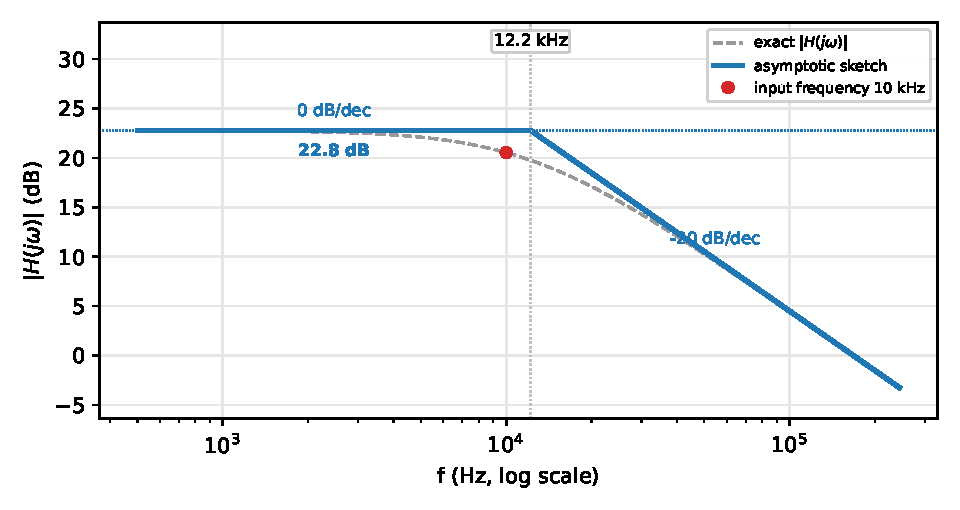
\includegraphics[width=0.78\linewidth,height=6.5cm,keepaspectratio]{p12_bode}\end{center}

{\small Blue: the straight-line sketch you are expected to draw. Dashed grey: the exact curve (about 3\,dB below the corner of an isolated pole). Red dot: the input frequency of Step 7.}
\solstep{7}{Steady-state output}The input is $V_i(t) = 0.02\sin\left(2\pi\cdot 10000\,t\right)$, so $\omega_{in} = 2\pi\cdot 10000 = 62800$\,rad/s. Put $s=j\omega_{in}$ in each factor (tool T5): magnitudes multiply, angles add.
{\small Rules: $\left|\frac{s}{s+p}\right| = \frac{\omega}{\sqrt{\omega^2+p^2}}$, $\angle = \frac{\pi}{2}-\tan^{-1}\frac{\omega}{p}$;\quad $\left|\frac{1}{1+s/p}\right| = \frac{1}{\sqrt{1+(\omega/p)^2}}$, $\angle = -\tan^{-1}\frac{\omega}{p}$;\quad $\left|1+\frac{s}{z}\right| = \sqrt{1+(\omega/z)^2}$, $\angle = \tan^{-1}\frac{\omega}{z}$;\quad a negative $K$ adds $-\pi$.}
\begin{center}\renewcommand{\arraystretch}{1.35}
\begin{tabular}{ccc}
\toprule
factor & magnitude & angle (rad) \\
\midrule
$13.8$ & $13.75$ & $0$ \\
$\rule[-1.7em]{0pt}{4em}\dfrac{1}{1+\dfrac{s}{2\pi\cdot 12.2\mathrm{k}}}$ & $0.7735$ & $-0.687$ \\
\textbf{total} & $\mathbf{10.64}$ (product) & $\mathbf{-0.687}$ (sum) \\
\bottomrule
\end{tabular}\end{center}

\begin{align*}
|H(j\omega_{in})| &= 10.6, \qquad \angle H(j\omega_{in}) = -0.687\ \mathrm{rad} \\
v_{o,ac}(t) &= 10.6\times 0.02\,\sin\left(2\pi\cdot 10000\,t - 0.687\right) = 0.213\,\sin\left(2\pi\cdot 10000\,t - 0.687\right)
\end{align*}

\[
\boxed{V_o(t) = 0.213\,\sin\left(2\pi\cdot 10000\,t - 0.687\right)\ \mathrm{V}}
\]

\begin{ansbox}
$H(s) = 13.8\,\dfrac{1}{1+\dfrac{s}{2\pi\cdot 12.2\mathrm{k}}}$\quad (corners: 12.2 kHz)\\[4pt]
$V_o(t) = 0.213\,\sin\left(2\pi\cdot 10000\,t - 0.687\right)\ \mathrm{V}$
\end{ansbox}

\newpage
\subsection*{Solution 4D.13 \hfill Hard}
\begin{center}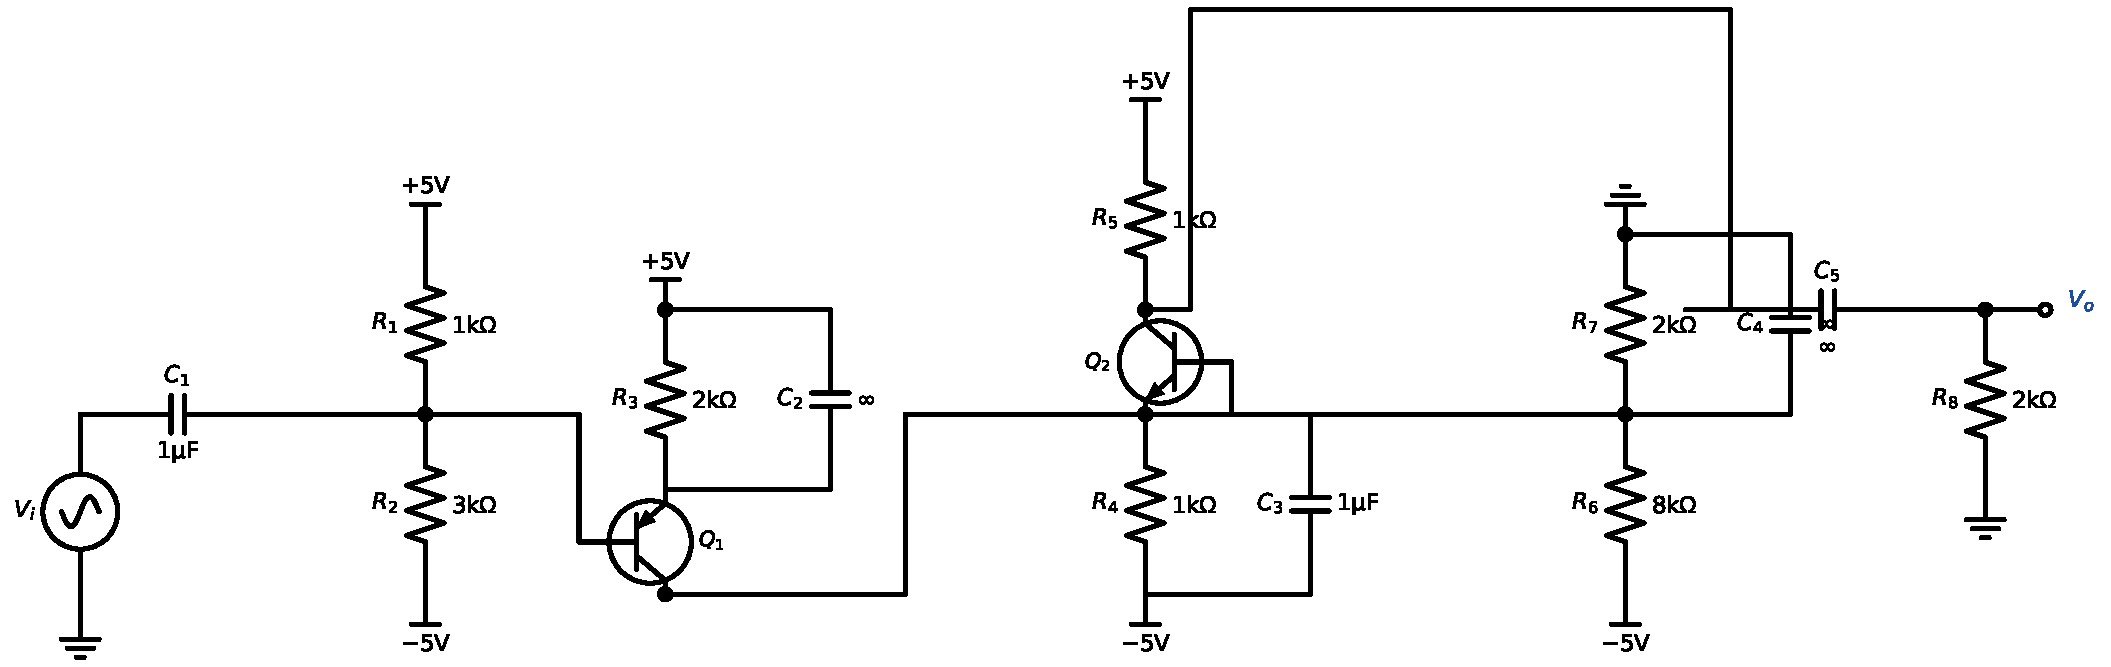
\includegraphics[width=0.9\linewidth,height=6cm,keepaspectratio]{p13_circuit}\end{center}
\solstep{1}{DC currents and small-signal parameters}The DC collector currents are given: $I_{C1} = 900\,\mu \mathrm{A}$, $I_{C2} = 2.4\,\mathrm{m}\mathrm{A}$. For AC every DC supply is ground and every ``$\infty$'' capacitor is a short (tool T3). Small-signal emitter resistances (tool T3):\begin{align*}
r_{e1} &= \frac{V_T}{I_{C1}} = \frac{25\,\mathrm{mV}}{900\,\mu \mathrm{A}} = 27.8\,\Omega \\
r_{e2} &= \frac{V_T}{I_{C2}} = \frac{25\,\mathrm{mV}}{2.4\,\mathrm{m}\mathrm{A}} = 10.4\,\Omega
\end{align*}

\solstep{2}{Input resistance of each stage}Input resistance of every stage, from the last stage back to the first (each one loads the stage before it; tool T4):\begin{align*}
R_{i1} &= Z_{base,1} = (\beta+1)(r_{e1} + 0) = 2.81\,\mathrm{k}\Omega \\
R_{i2} &= Z_{emitter,2} = r_{e2} + \frac{0}{\beta+1} = 10.4\,\Omega
\end{align*}

\solstep{3}{Gain along the signal path}Multiply the node-to-node gains along the signal path (tool T4):\[
H(s) = \frac{v_{b1}}{v_i}\cdot\frac{v_{c1}}{v_{b1}}\cdot\frac{v_{c2}}{v_{e2}}
\]
\begin{align*}
\frac{v_{b1}}{v_i} &= \frac{R_{1} \parallel R_{2} \parallel R_{i1}}{\frac{1}{sC_{1}} + R_{1} \parallel R_{2} \parallel R_{i1}} = \dfrac{s}{s + 1690} \\
\frac{v_{c1}}{v_{b1}} &= -\alpha\frac{Z_{C1}}{r_{e1} + Z_{E1}},\quad Z_{C1} = R_{4} \parallel \frac{1}{sC_{3}} \parallel R_{i2},\ Z_{E1} = 0\ \Rightarrow\ \dfrac{-35600}{s + 97000} \\
\frac{v_{c2}}{v_{e2}} &= \alpha\frac{Z_{C2}}{Z_{emitter,2}},\quad Z_{C2} = R_{5} \parallel R_{8}\ \Rightarrow\ 63.4
\end{align*}

\solstep{4}{Transfer function}Multiply and simplify:\[
H(s) = \dfrac{-2.26\times 10^{6}\,s}{s^{2} + 98700\,s + 1.64\times 10^{8}}
\]

\solstep{5}{Standard (Bode-ready) form}Find the roots. Every root $s=-p$ of the denominator is a \emph{pole}, every root $s=-z$ of the numerator is a \emph{zero}; $|p|$ and $|z|$ are the corner frequencies (rad/s).
\begin{itemize}[leftmargin=*,itemsep=2pt]
\item Numerator: it has the factor $s$ $\Rightarrow$ 1 zero at $s=0$.
\item Denominator: $s^{2} + 98700\,s + 1.64\times 10^{8}$; quadratic formula:\[
s = \frac{-98700 \pm \sqrt{(98700)^2 - 4(1.64\times 10^{8})}}{2} = \frac{-98700 \pm 95300}{2} \Rightarrow s = -1690,\ -97000
\]

\end{itemize}

Factored form (leading coefficient in front):
\[
H(s) = -2.26\times 10^{6}\,\dfrac{s}{(s+1690)(s+97000)}
\]

Bode-ready form: rewrite every $(s+p) = p\left(1+\frac{s}{p}\right)$ and $(s+z) = z\left(1+\frac{s}{z}\right)$, and collect all constants into $K$. Each $s$ in the numerator is paired with one of the \emph{lowest} poles as $\frac{s}{s+p}$ (that factor is $\approx 1$ above $p$). Then every factor except $K$ is $\approx 1$ inside the pass-band:
\[
H(s) = -23.3\,\dfrac{s}{s+2\pi\cdot 269}\,\dfrac{1}{1+\dfrac{s}{2\pi\cdot 15.4\mathrm{k}}},\qquad K = -23.3
\]

\begin{center}\renewcommand{\arraystretch}{1.35}
\begin{tabular}{cccc}
\toprule
type & $\omega_c$ (rad/s) & $f_c=\omega_c/2\pi$ & slope change \\
\midrule
pole & $1690$ & 269 Hz & $-20$ dB/dec \\
pole & $97000$ & 15.4 kHz & $-20$ dB/dec \\
\bottomrule
\end{tabular}\end{center}

\solstep{6}{Magnitude Bode plot}Below every corner $|H(s)|\approx 0.0138\,s$, so the plot starts with a slope of $+20$\,dB/dec. Then, moving right, each pole bends the line down by 20\,dB/dec and each zero bends it up by 20\,dB/dec (tool T6):
\begin{center}\renewcommand{\arraystretch}{1.35}
\begin{tabular}{lcl}
\toprule
frequency range & slope & asymptote level \\
\midrule
$f<$ 269 Hz & $+20$ dB/dec & 27.3 dB at end \\
269 Hz -- 15.4 kHz & $0$ dB/dec (flat) & 27.3 dB at start, 27.3 dB at end \\
$f>$ 15.4 kHz & $-20$ dB/dec & 27.3 dB at start \\
\bottomrule
\end{tabular}\end{center}

The flat (pass-band) level is $20\log_{10}|K| = 20\log_{10}23.3 = 27.3$\,dB.
\begin{center}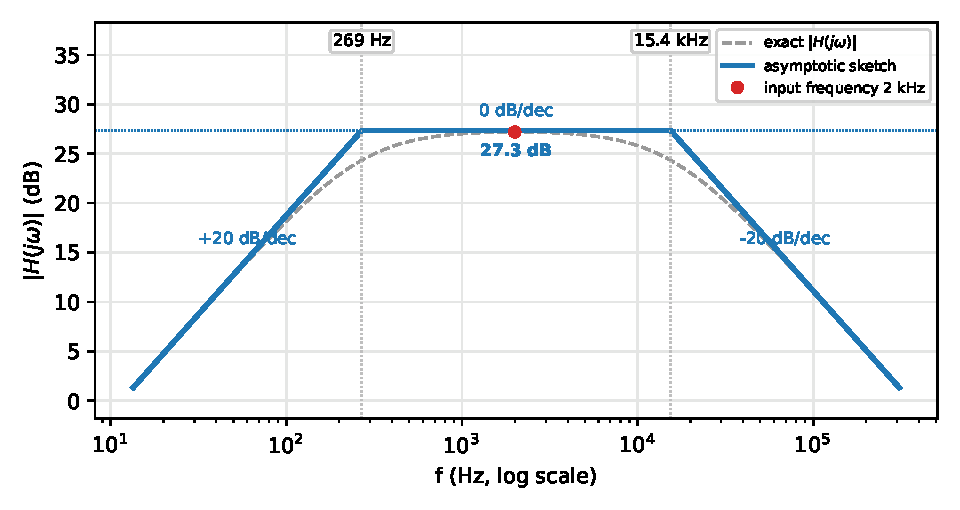
\includegraphics[width=0.78\linewidth,height=6.5cm,keepaspectratio]{p13_bode}\end{center}

{\small Blue: the straight-line sketch you are expected to draw. Dashed grey: the exact curve (about 3\,dB below the corner of an isolated pole). Red dot: the input frequency of Step 7.}
\solstep{7}{Steady-state output}The input is $V_i(t) = 0.005\sin\left(2\pi\cdot 2000\,t\right)$, so $\omega_{in} = 2\pi\cdot 2000 = 12600$\,rad/s. Put $s=j\omega_{in}$ in each factor (tool T5): magnitudes multiply, angles add.
{\small Rules: $\left|\frac{s}{s+p}\right| = \frac{\omega}{\sqrt{\omega^2+p^2}}$, $\angle = \frac{\pi}{2}-\tan^{-1}\frac{\omega}{p}$;\quad $\left|\frac{1}{1+s/p}\right| = \frac{1}{\sqrt{1+(\omega/p)^2}}$, $\angle = -\tan^{-1}\frac{\omega}{p}$;\quad $\left|1+\frac{s}{z}\right| = \sqrt{1+(\omega/z)^2}$, $\angle = \tan^{-1}\frac{\omega}{z}$;\quad a negative $K$ adds $-\pi$.}
\begin{center}\renewcommand{\arraystretch}{1.35}
\begin{tabular}{ccc}
\toprule
factor & magnitude & angle (rad) \\
\midrule
$-23.3$ & $23.28$ & $-3.14$ \\
$\rule[-1.1em]{0pt}{2.8em}\dfrac{s}{s+2\pi\cdot 269}$ & $0.9911$ & $0.134$ \\
$\rule[-1.7em]{0pt}{4em}\dfrac{1}{1+\dfrac{s}{2\pi\cdot 15.4\mathrm{k}}}$ & $0.9917$ & $-0.129$ \\
\textbf{total} & $\mathbf{22.89}$ (product) & $\mathbf{-3.14}$ (sum) \\
\bottomrule
\end{tabular}\end{center}

\begin{align*}
|H(j\omega_{in})| &= 22.9, \qquad \angle H(j\omega_{in}) = -3.14\ \mathrm{rad} \\
v_{o,ac}(t) &= 22.9\times 0.005\,\sin\left(2\pi\cdot 2000\,t - 3.14\right) = 0.114\,\sin\left(2\pi\cdot 2000\,t - 3.14\right)
\end{align*}

\[
\boxed{V_o(t) = 0.114\,\sin\left(2\pi\cdot 2000\,t - 3.14\right)\ \mathrm{V}}
\]

\begin{ansbox}
$H(s) = -23.3\,\dfrac{s}{s+2\pi\cdot 269}\,\dfrac{1}{1+\dfrac{s}{2\pi\cdot 15.4\mathrm{k}}}$\quad (corners: 269 Hz, 15.4 kHz)\\[4pt]
$V_o(t) = 0.114\,\sin\left(2\pi\cdot 2000\,t - 3.14\right)\ \mathrm{V}$
\end{ansbox}

\newpage
\subsection*{Solution 4D.14 \hfill Hard}
\begin{center}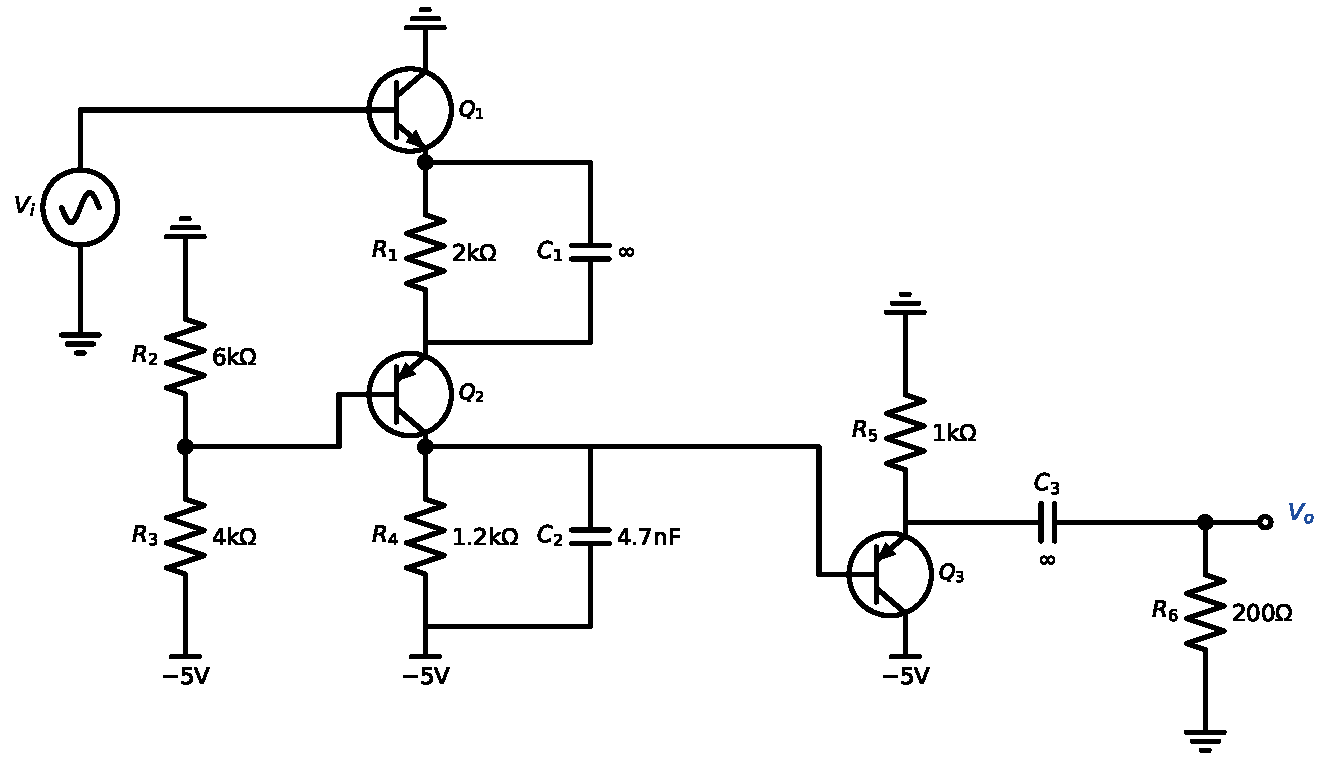
\includegraphics[width=0.9\linewidth,height=6cm,keepaspectratio]{p14_circuit}\end{center}
\solstep{1}{DC currents and small-signal parameters}The DC collector currents are given: $I_{C1} = 800\,\mu \mathrm{A}$, $I_{C2} = 800\,\mu \mathrm{A}$, $I_{C3} = 3.34\,\mathrm{m}\mathrm{A}$. For AC every DC supply is ground and every ``$\infty$'' capacitor is a short (tool T3). Small-signal emitter resistances (tool T3):\begin{align*}
r_{e1} &= \frac{V_T}{I_{C1}} = \frac{25\,\mathrm{mV}}{800\,\mu \mathrm{A}} = 31.2\,\Omega \\
r_{e2} &= \frac{V_T}{I_{C2}} = \frac{25\,\mathrm{mV}}{800\,\mu \mathrm{A}} = 31.2\,\Omega \\
r_{e3} &= \frac{V_T}{I_{C3}} = \frac{25\,\mathrm{mV}}{3.34\,\mathrm{m}\mathrm{A}} = 7.49\,\Omega
\end{align*}

\solstep{2}{Input resistance of each stage}Input resistance of every stage, from the last stage back to the first (each one loads the stage before it; tool T4):\begin{align*}
R_{i1} &= Z_{base,1} = (\beta+1)(r_{e1} + R_{i2}) = 8.71\,\mathrm{k}\Omega \\
R_{i2} &= Z_{emitter,2} = r_{e2} + \frac{R_{2} \parallel R_{3}}{\beta+1} = 55\,\Omega \\
R_{i3} &= Z_{base,3} = (\beta+1)(r_{e3} + R_{5} \parallel R_{6}) = 17.6\,\mathrm{k}\Omega
\end{align*}

\solstep{3}{Gain along the signal path}Multiply the node-to-node gains along the signal path (tool T4):\[
H(s) = \frac{v_{e1}}{v_{b1}}\cdot\frac{v_{c2}}{v_{e2}}\cdot\frac{v_{e3}}{v_{b3}}
\]
\begin{align*}
\frac{v_{e1}}{v_{b1}} &= \frac{Z_{E1}}{r_{e1} + Z_{E1}},\quad Z_{E1} = R_{i2}\ \Rightarrow\ 0.638 \\
\frac{v_{c2}}{v_{e2}} &= \alpha\frac{Z_{C2}}{Z_{emitter,2}},\quad Z_{C2} = R_{4} \parallel \frac{1}{sC_{2}} \parallel R_{i3}\ \Rightarrow\ \dfrac{3.83\times 10^{6}}{s + 1.89\times 10^{5}} \\
\frac{v_{e3}}{v_{b3}} &= \frac{Z_{E3}}{r_{e3} + Z_{E3}},\quad Z_{E3} = R_{5} \parallel R_{6}\ \Rightarrow\ 0.957
\end{align*}

\solstep{4}{Transfer function}Multiply and simplify:\[
H(s) = \dfrac{2.34\times 10^{6}}{s + 1.89\times 10^{5}}
\]

\solstep{5}{Standard (Bode-ready) form}Find the roots. Every root $s=-p$ of the denominator is a \emph{pole}, every root $s=-z$ of the numerator is a \emph{zero}; $|p|$ and $|z|$ are the corner frequencies (rad/s).
\begin{itemize}[leftmargin=*,itemsep=2pt]
\item Denominator: $s + 1.89\times 10^{5}$; $s + 1.89\times 10^{5} = 0 \Rightarrow s = -1.89\times 10^{5}$.
\end{itemize}

Factored form (leading coefficient in front):
\[
H(s) = 2.34\times 10^{6}\,\dfrac{1}{(s+1.89\times 10^{5})}
\]

Bode-ready form: rewrite every $(s+p) = p\left(1+\frac{s}{p}\right)$ and $(s+z) = z\left(1+\frac{s}{z}\right)$, and collect all constants into $K$. Then every factor except $K$ is $\approx 1$ inside the pass-band:
\[
H(s) = 12.3\,\dfrac{1}{1+\dfrac{s}{2\pi\cdot 30.1\mathrm{k}}},\qquad K = 12.3
\]

\begin{center}\renewcommand{\arraystretch}{1.35}
\begin{tabular}{cccc}
\toprule
type & $\omega_c$ (rad/s) & $f_c=\omega_c/2\pi$ & slope change \\
\midrule
pole & $1.89\times 10^{5}$ & 30.1 kHz & $-20$ dB/dec \\
\bottomrule
\end{tabular}\end{center}

\solstep{6}{Magnitude Bode plot}Below every corner, all factors are $\approx$ constant: $|H| \approx 12.3$ $= 21.8$\,dB (flat, 0 dB/dec). Then, moving right, each pole bends the line down by 20\,dB/dec and each zero bends it up by 20\,dB/dec (tool T6):
\begin{center}\renewcommand{\arraystretch}{1.35}
\begin{tabular}{lcl}
\toprule
frequency range & slope & asymptote level \\
\midrule
$f<$ 30.1 kHz & $0$ dB/dec (flat) & 21.8 dB at end \\
$f>$ 30.1 kHz & $-20$ dB/dec & 21.8 dB at start \\
\bottomrule
\end{tabular}\end{center}

The flat (pass-band) level is $20\log_{10}|K| = 20\log_{10}12.3 = 21.8$\,dB.
\begin{center}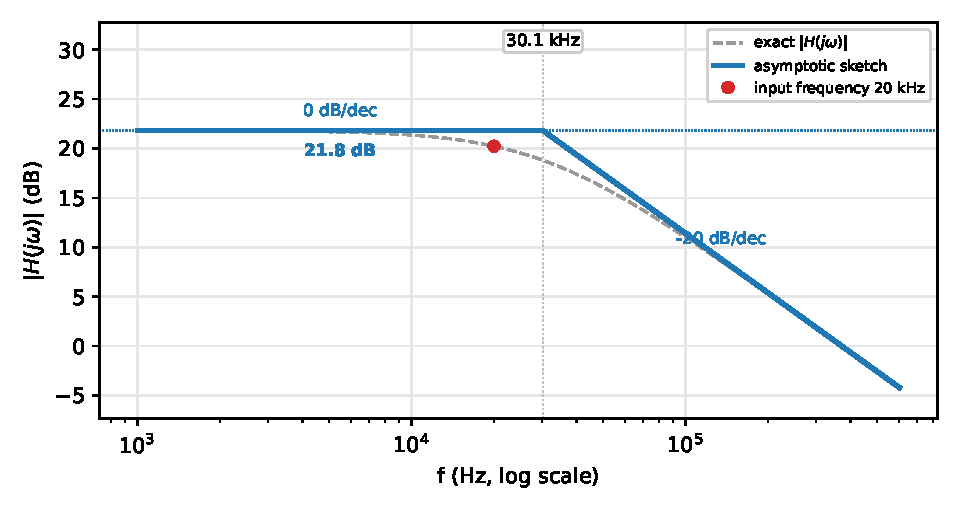
\includegraphics[width=0.78\linewidth,height=6.5cm,keepaspectratio]{p14_bode}\end{center}

{\small Blue: the straight-line sketch you are expected to draw. Dashed grey: the exact curve (about 3\,dB below the corner of an isolated pole). Red dot: the input frequency of Step 7.}
\solstep{7}{Steady-state output}The input is $V_i(t) = 0.05\sin\left(2\pi\cdot 20000\,t+\frac{\pi}{4}\right)$, so $\omega_{in} = 2\pi\cdot 20000 = 1.26\times 10^{5}$\,rad/s. Put $s=j\omega_{in}$ in each factor (tool T5): magnitudes multiply, angles add.
{\small Rules: $\left|\frac{s}{s+p}\right| = \frac{\omega}{\sqrt{\omega^2+p^2}}$, $\angle = \frac{\pi}{2}-\tan^{-1}\frac{\omega}{p}$;\quad $\left|\frac{1}{1+s/p}\right| = \frac{1}{\sqrt{1+(\omega/p)^2}}$, $\angle = -\tan^{-1}\frac{\omega}{p}$;\quad $\left|1+\frac{s}{z}\right| = \sqrt{1+(\omega/z)^2}$, $\angle = \tan^{-1}\frac{\omega}{z}$;\quad a negative $K$ adds $-\pi$.}
\begin{center}\renewcommand{\arraystretch}{1.35}
\begin{tabular}{ccc}
\toprule
factor & magnitude & angle (rad) \\
\midrule
$12.3$ & $12.34$ & $0$ \\
$\rule[-1.7em]{0pt}{4em}\dfrac{1}{1+\dfrac{s}{2\pi\cdot 30.1\mathrm{k}}}$ & $0.8333$ & $-0.586$ \\
\textbf{total} & $\mathbf{10.28}$ (product) & $\mathbf{-0.586}$ (sum) \\
\bottomrule
\end{tabular}\end{center}

\begin{align*}
|H(j\omega_{in})| &= 10.3, \qquad \angle H(j\omega_{in}) = -0.586\ \mathrm{rad} \\
v_{o,ac}(t) &= 10.3\times 0.05\,\sin\left(2\pi\cdot 20000\,t + 0.2\right) = 0.514\,\sin\left(2\pi\cdot 20000\,t + 0.2\right)
\end{align*}

(phase: $\theta + \angle H = \frac{\pi}{4} + (-0.586) = 0.2$\,rad.)
\[
\boxed{V_o(t) = 0.514\,\sin\left(2\pi\cdot 20000\,t + 0.2\right)\ \mathrm{V}}
\]

\begin{ansbox}
$H(s) = 12.3\,\dfrac{1}{1+\dfrac{s}{2\pi\cdot 30.1\mathrm{k}}}$\quad (corners: 30.1 kHz)\\[4pt]
$V_o(t) = 0.514\,\sin\left(2\pi\cdot 20000\,t + 0.2\right)\ \mathrm{V}$
\end{ansbox}

\newpage
\subsection*{Solution 4D.15 \hfill Hard}
\begin{center}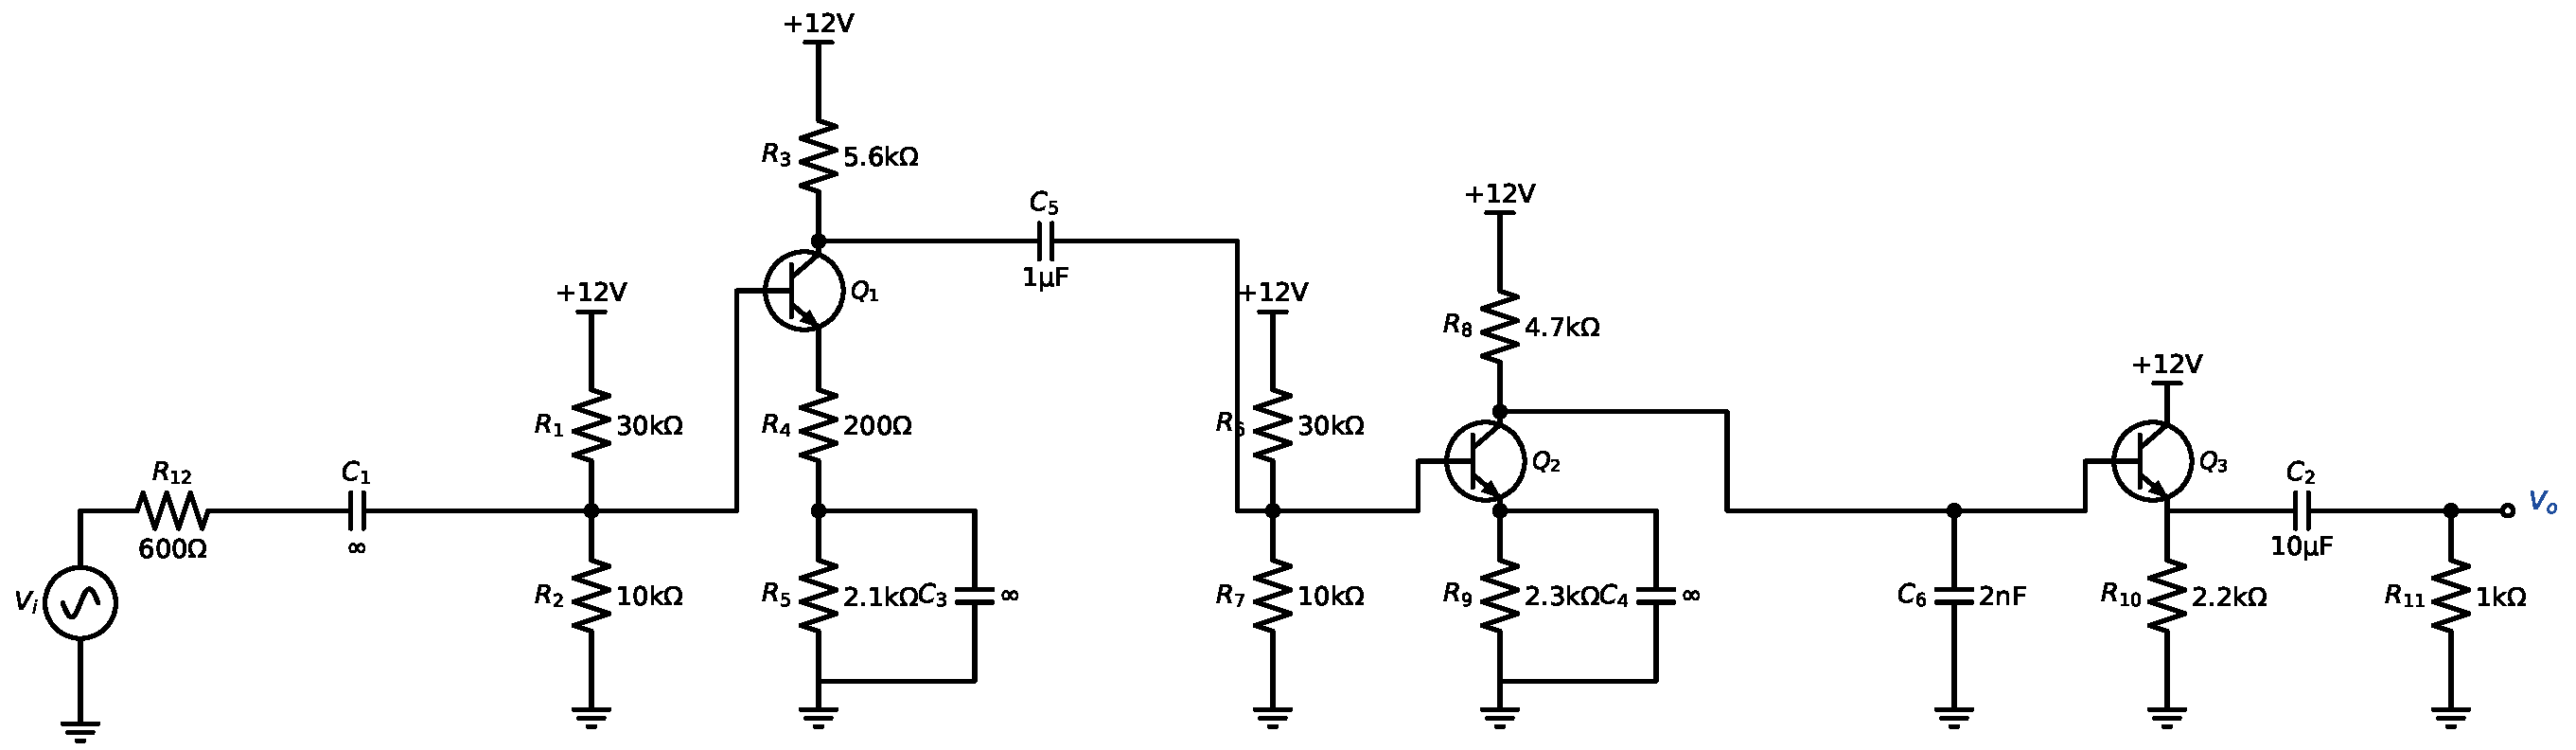
\includegraphics[width=0.9\linewidth,height=6cm,keepaspectratio]{p15_circuit}\end{center}
\solstep{1}{DC currents and small-signal parameters}The DC collector currents are given: $I_{C1} = 1\,\mathrm{m}\mathrm{A}$, $I_{C2} = 1\,\mathrm{m}\mathrm{A}$, $I_{C3} = 3\,\mathrm{m}\mathrm{A}$. For AC every DC supply is ground and every ``$\infty$'' capacitor is a short (tool T3). Small-signal emitter resistances (tool T3):\begin{align*}
r_{e1} &= \frac{V_T}{I_{C1}} = \frac{25\,\mathrm{mV}}{1\,\mathrm{m}\mathrm{A}} = 25\,\Omega \\
r_{e2} &= \frac{V_T}{I_{C2}} = \frac{25\,\mathrm{mV}}{1\,\mathrm{m}\mathrm{A}} = 25\,\Omega \\
r_{e3} &= \frac{V_T}{I_{C3}} = \frac{25\,\mathrm{mV}}{3\,\mathrm{m}\mathrm{A}} = 8.33\,\Omega
\end{align*}

\solstep{2}{Input resistance of each stage}Input resistance of every stage, from the last stage back to the first (each one loads the stage before it; tool T4):\begin{align*}
R_{i1} &= Z_{base,1} = (\beta+1)(r_{e1} + R_{4}) = 22.7\,\mathrm{k}\Omega \\
R_{i2} &= Z_{base,2} = (\beta+1)(r_{e2} + 0) = 2.52\,\mathrm{k}\Omega \\
R_{i3} &= Z_{base,3} = (\beta+1)(r_{e3} + R_{10} \parallel \left(\frac{1}{sC_{2}} + R_{11}\right)) = \dfrac{70300\,s + 6.97\times 10^{6}}{s + 31.2}
\end{align*}

\solstep{3}{Gain along the signal path}Multiply the node-to-node gains along the signal path (tool T4):\[
H(s) = \frac{v_{b1}}{v_i}\cdot\frac{v_{c1}}{v_{b1}}\cdot\frac{v_{b2}}{v_{c1}}\cdot\frac{v_{c2}}{v_{b2}}\cdot\frac{v_{e3}}{v_{b3}}\cdot\frac{v_o}{v_{e3}}
\]
\begin{align*}
\frac{v_{b1}}{v_i} &= \frac{R_{1} \parallel R_{2} \parallel R_{i1}}{R_{12} + R_{1} \parallel R_{2} \parallel R_{i1}} = 0.904 \\
\frac{v_{c1}}{v_{b1}} &= -\alpha\frac{Z_{C1}}{r_{e1} + Z_{E1}},\quad Z_{C1} = R_{3} \parallel \left(\frac{1}{sC_{5}} + \left(R_{6} \parallel R_{7} \parallel R_{i2}\right)\right),\ Z_{E1} = R_{4}\ \Rightarrow\ \dfrac{-6.22\,s - 3290}{s + 134} \\
\frac{v_{b2}}{v_{c1}} &= \frac{R_{6} \parallel R_{7} \parallel R_{i2}}{\frac{1}{sC_{5}} + R_{6} \parallel R_{7} \parallel R_{i2}} = \dfrac{s}{s + 529} \\
\frac{v_{c2}}{v_{b2}} &= -\alpha\frac{Z_{C2}}{r_{e2} + Z_{E2}},\quad Z_{C2} = R_{8} \parallel \frac{1}{sC_{6}} \parallel R_{i3},\ Z_{E2} = 0\ \Rightarrow\ \dfrac{-1.98\times 10^{7}\,s - 1.96\times 10^{9}}{s^{2} + 1.14\times 10^{5}\,s + 1.08\times 10^{7}} \\
\frac{v_{e3}}{v_{b3}} &= \frac{Z_{E3}}{r_{e3} + Z_{E3}},\quad Z_{E3} = R_{10} \parallel \left(\frac{1}{sC_{2}} + R_{11}\right)\ \Rightarrow\ \dfrac{0.988\,s + 98.8}{s + 99.2} \\
\frac{v_o}{v_{e3}} &= \frac{R_{11}}{\frac{1}{sC_{2}} + R_{11}} = \dfrac{s}{s + 100}
\end{align*}

\solstep{4}{Transfer function}Multiply and simplify:\[
H(s) = \dfrac{1.1\times 10^{8}\,s^{2}}{s^{3} + 1.14\times 10^{5}\,s^{2} + 2.59\times 10^{7}\,s + 1.44\times 10^{9}}
\]

\solstep{5}{Standard (Bode-ready) form}Find the roots. Every root $s=-p$ of the denominator is a \emph{pole}, every root $s=-z$ of the numerator is a \emph{zero}; $|p|$ and $|z|$ are the corner frequencies (rad/s).
\begin{itemize}[leftmargin=*,itemsep=2pt]
\item Numerator: it has the factor $s^2$ $\Rightarrow$ 2 zeros at $s=0$.
\item Denominator: $s^{3} + 1.14\times 10^{5}\,s^{2} + 2.59\times 10^{7}\,s + 1.44\times 10^{9}$; this is degree 3: use a calculator's polynomial solver (or \texttt{numpy.roots}) $\Rightarrow s = -94.9,\ -134,\ -1.14\times 10^{5}$.
\end{itemize}

Factored form (leading coefficient in front):
\[
H(s) = 1.1\times 10^{8}\,\dfrac{s^{2}}{(s+94.9)(s+134)(s+1.14\times 10^{5})}
\]

Bode-ready form: rewrite every $(s+p) = p\left(1+\frac{s}{p}\right)$ and $(s+z) = z\left(1+\frac{s}{z}\right)$, and collect all constants into $K$. Each $s$ in the numerator is paired with one of the \emph{lowest} poles as $\frac{s}{s+p}$ (that factor is $\approx 1$ above $p$). Then every factor except $K$ is $\approx 1$ inside the pass-band:
\[
H(s) = 968\,\dfrac{s}{s+2\pi\cdot 15.1}\,\dfrac{s}{s+2\pi\cdot 21.3}\,\dfrac{1}{1+\dfrac{s}{2\pi\cdot 18.1\mathrm{k}}},\qquad K = 968
\]

\begin{center}\renewcommand{\arraystretch}{1.35}
\begin{tabular}{cccc}
\toprule
type & $\omega_c$ (rad/s) & $f_c=\omega_c/2\pi$ & slope change \\
\midrule
pole & $94.9$ & 15.1 Hz & $-20$ dB/dec \\
pole & $134$ & 21.3 Hz & $-20$ dB/dec \\
pole & $1.14\times 10^{5}$ & 18.1 kHz & $-20$ dB/dec \\
\bottomrule
\end{tabular}\end{center}

\solstep{6}{Magnitude Bode plot}Below every corner $|H(s)|\approx 0.0764\,s^2$, so the plot starts with a slope of $+40$\,dB/dec. Then, moving right, each pole bends the line down by 20\,dB/dec and each zero bends it up by 20\,dB/dec (tool T6):
\begin{center}\renewcommand{\arraystretch}{1.35}
\begin{tabular}{lcl}
\toprule
frequency range & slope & asymptote level \\
\midrule
$f<$ 15.1 Hz & $+40$ dB/dec & 56.8 dB at end \\
15.1 Hz -- 21.3 Hz & $+20$ dB/dec & 56.8 dB at start, 59.7 dB at end \\
21.3 Hz -- 18.1 kHz & $0$ dB/dec (flat) & 59.7 dB at start, 59.7 dB at end \\
$f>$ 18.1 kHz & $-20$ dB/dec & 59.7 dB at start \\
\bottomrule
\end{tabular}\end{center}

The flat (pass-band) level is $20\log_{10}|K| = 20\log_{10}968 = 59.7$\,dB.
\begin{center}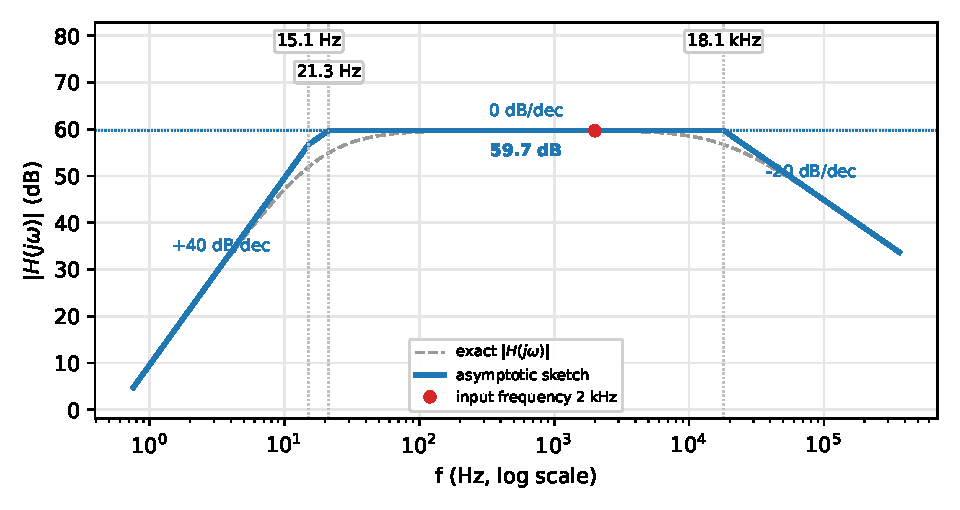
\includegraphics[width=0.78\linewidth,height=6.5cm,keepaspectratio]{p15_bode}\end{center}

{\small Blue: the straight-line sketch you are expected to draw. Dashed grey: the exact curve (about 3\,dB below the corner of an isolated pole). Red dot: the input frequency of Step 7.}
\solstep{7}{Steady-state output}The input is $V_i(t) = 5\times 10^{-4}\sin\left(2\pi\cdot 2000\,t\right)$, so $\omega_{in} = 2\pi\cdot 2000 = 12600$\,rad/s. Put $s=j\omega_{in}$ in each factor (tool T5): magnitudes multiply, angles add.
{\small Rules: $\left|\frac{s}{s+p}\right| = \frac{\omega}{\sqrt{\omega^2+p^2}}$, $\angle = \frac{\pi}{2}-\tan^{-1}\frac{\omega}{p}$;\quad $\left|\frac{1}{1+s/p}\right| = \frac{1}{\sqrt{1+(\omega/p)^2}}$, $\angle = -\tan^{-1}\frac{\omega}{p}$;\quad $\left|1+\frac{s}{z}\right| = \sqrt{1+(\omega/z)^2}$, $\angle = \tan^{-1}\frac{\omega}{z}$;\quad a negative $K$ adds $-\pi$.}
\begin{center}\renewcommand{\arraystretch}{1.35}
\begin{tabular}{ccc}
\toprule
factor & magnitude & angle (rad) \\
\midrule
$968$ & $968.4$ & $0$ \\
$\rule[-1.1em]{0pt}{2.8em}\dfrac{s}{s+2\pi\cdot 15.1}$ & $1$ & $0.00755$ \\
$\rule[-1.1em]{0pt}{2.8em}\dfrac{s}{s+2\pi\cdot 21.3}$ & $0.9999$ & $0.0106$ \\
$\rule[-1.7em]{0pt}{4em}\dfrac{1}{1+\dfrac{s}{2\pi\cdot 18.1\mathrm{k}}}$ & $0.9939$ & $-0.11$ \\
\textbf{total} & $\mathbf{962.4}$ (product) & $\mathbf{-0.0921}$ (sum) \\
\bottomrule
\end{tabular}\end{center}

\begin{align*}
|H(j\omega_{in})| &= 962, \qquad \angle H(j\omega_{in}) = -0.0921\ \mathrm{rad} \\
v_{o,ac}(t) &= 962\times 5\times 10^{-4}\,\sin\left(2\pi\cdot 2000\,t - 0.0921\right) = 0.481\,\sin\left(2\pi\cdot 2000\,t - 0.0921\right)
\end{align*}

\[
\boxed{V_o(t) = 0.481\,\sin\left(2\pi\cdot 2000\,t - 0.0921\right)\ \mathrm{V}}
\]

\begin{ansbox}
$H(s) = 968\,\dfrac{s}{s+2\pi\cdot 15.1}\,\dfrac{s}{s+2\pi\cdot 21.3}\,\dfrac{1}{1+\dfrac{s}{2\pi\cdot 18.1\mathrm{k}}}$\quad (corners: 15.1 Hz, 21.3 Hz, 18.1 kHz)\\[4pt]
$V_o(t) = 0.481\,\sin\left(2\pi\cdot 2000\,t - 0.0921\right)\ \mathrm{V}$
\end{ansbox}

\newpage
\subsection*{Solution 4D.16 \hfill Hard}
\begin{center}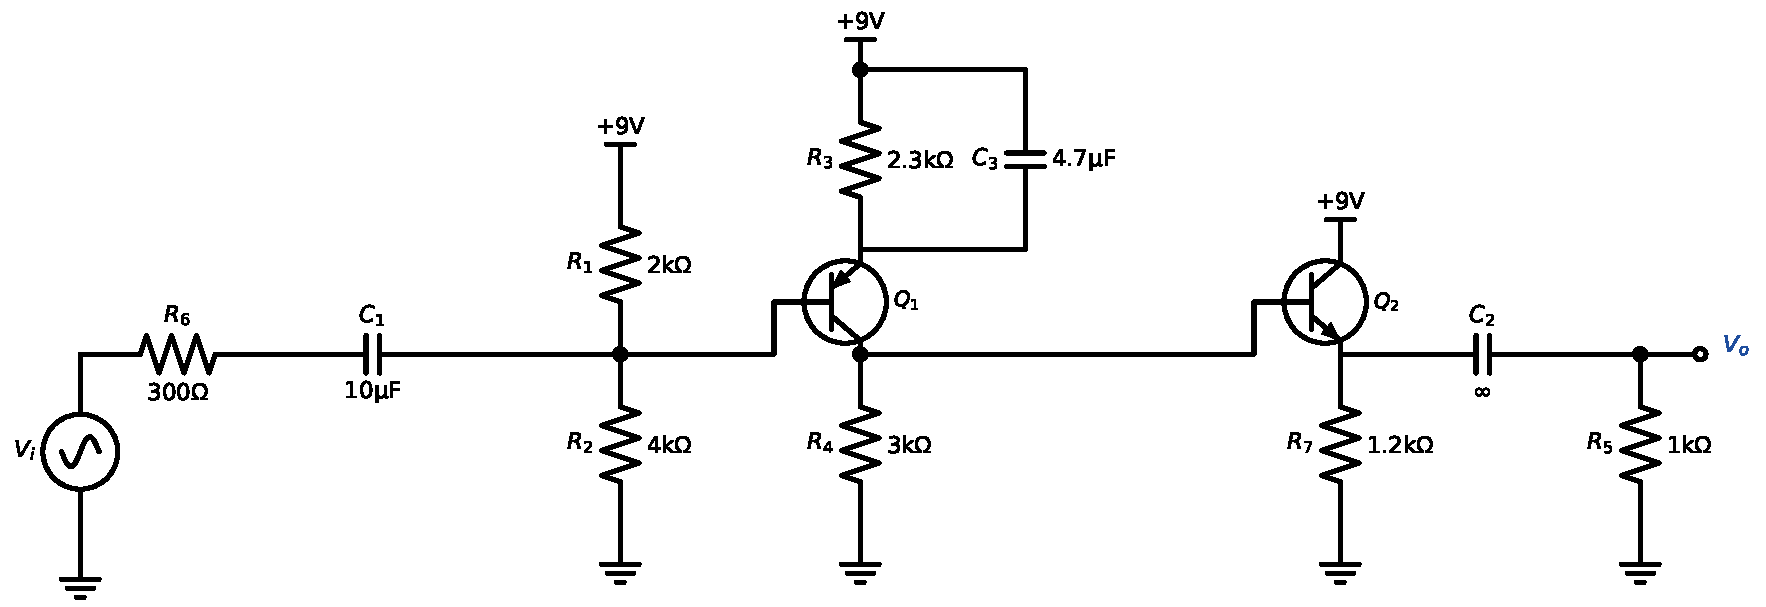
\includegraphics[width=0.9\linewidth,height=6cm,keepaspectratio]{p16_circuit}\end{center}
\solstep{1}{DC currents and small-signal parameters}The DC collector currents are given: $I_{C1} = 1\,\mathrm{m}\mathrm{A}$, $I_{C2} = 1.92\,\mathrm{m}\mathrm{A}$. For AC every DC supply is ground and every ``$\infty$'' capacitor is a short (tool T3). Small-signal emitter resistances (tool T3):\begin{align*}
r_{e1} &= \frac{V_T}{I_{C1}} = \frac{25\,\mathrm{mV}}{1\,\mathrm{m}\mathrm{A}} = 25\,\Omega \\
r_{e2} &= \frac{V_T}{I_{C2}} = \frac{25\,\mathrm{mV}}{1.92\,\mathrm{m}\mathrm{A}} = 13\,\Omega
\end{align*}

\solstep{2}{Input resistance of each stage}Input resistance of every stage, from the last stage back to the first (each one loads the stage before it; tool T4):\begin{align*}
R_{i1} &= Z_{base,1} = (\beta+1)(r_{e1} + R_{3} \parallel \frac{1}{sC_{3}}) = \dfrac{2520\,s + 2.17\times 10^{7}}{s + 92.5} \\
R_{i2} &= Z_{base,2} = (\beta+1)(r_{e2} + R_{7} \parallel R_{5}) = 56.4\,\mathrm{k}\Omega
\end{align*}

\solstep{3}{Gain along the signal path}Multiply the node-to-node gains along the signal path (tool T4):\[
H(s) = \frac{v_{b1}}{v_i}\cdot\frac{v_{c1}}{v_{b1}}\cdot\frac{v_{e2}}{v_{b2}}
\]
\begin{align*}
\frac{v_{b1}}{v_i} &= \frac{R_{1} \parallel R_{2} \parallel R_{i1}}{R_{6} + \frac{1}{sC_{1}} + R_{1} \parallel R_{2} \parallel R_{i1}} = \dfrac{0.744\,s^{2} + 6400\,s}{s^{2} + 7940\,s + 4.83\times 10^{5}} \\
\frac{v_{c1}}{v_{b1}} &= -\alpha\frac{Z_{C1}}{r_{e1} + Z_{E1}},\quad Z_{C1} = R_{4} \parallel R_{i2},\ Z_{E1} = R_{3} \parallel \frac{1}{sC_{3}}\ \Rightarrow\ \dfrac{-113\,s - 10400}{s + 8600} \\
\frac{v_{e2}}{v_{b2}} &= \frac{Z_{E2}}{r_{e2} + Z_{E2}},\quad Z_{E2} = R_{7} \parallel R_{5}\ \Rightarrow\ 0.977
\end{align*}

\solstep{4}{Transfer function}Multiply and simplify:\[
H(s) = \dfrac{-82\,s^{2} - 7580\,s}{s^{2} + 7940\,s + 4.83\times 10^{5}}
\]

\solstep{5}{Standard (Bode-ready) form}Find the roots. Every root $s=-p$ of the denominator is a \emph{pole}, every root $s=-z$ of the numerator is a \emph{zero}; $|p|$ and $|z|$ are the corner frequencies (rad/s).
\begin{itemize}[leftmargin=*,itemsep=2pt]
\item Numerator: it has the factor $s$ $\Rightarrow$ 1 zero at $s=0$.
\item Numerator (after taking out the $s$ factor): $-82\,s - 7580$; divide by the leading coefficient $-82$ (this does not move the roots): $s + 92.5$; $s + 92.5 = 0 \Rightarrow s = -92.5$.
\item Denominator: $s^{2} + 7940\,s + 4.83\times 10^{5}$; quadratic formula:\[
s = \frac{-7940 \pm \sqrt{(7940)^2 - 4(4.83\times 10^{5})}}{2} = \frac{-7940 \pm 7810}{2} \Rightarrow s = -61.3,\ -7870
\]

\end{itemize}

Factored form (leading coefficient in front):
\[
H(s) = -82\,\dfrac{s(s+92.5)}{(s+61.3)(s+7870)}
\]

Bode-ready form: rewrite every $(s+p) = p\left(1+\frac{s}{p}\right)$ and $(s+z) = z\left(1+\frac{s}{z}\right)$, and collect all constants into $K$. Each $s$ in the numerator is paired with one of the \emph{lowest} poles as $\frac{s}{s+p}$ (that factor is $\approx 1$ above $p$). Then every factor except $K$ is $\approx 1$ inside the pass-band:
\[
H(s) = -0.963\,\dfrac{s}{s+2\pi\cdot 9.76}\,\left(1+\dfrac{s}{2\pi\cdot 14.7}\right)\,\dfrac{1}{1+\dfrac{s}{2\pi\cdot 1.25\mathrm{k}}},\qquad K = -0.963
\]

\begin{center}\renewcommand{\arraystretch}{1.35}
\begin{tabular}{cccc}
\toprule
type & $\omega_c$ (rad/s) & $f_c=\omega_c/2\pi$ & slope change \\
\midrule
pole & $61.3$ & 9.76 Hz & $-20$ dB/dec \\
zero & $92.5$ & 14.7 Hz & $+20$ dB/dec \\
pole & $7870$ & 1.25 kHz & $-20$ dB/dec \\
\bottomrule
\end{tabular}\end{center}

\solstep{6}{Magnitude Bode plot}Below every corner $|H(s)|\approx 0.0157\,s$, so the plot starts with a slope of $+20$\,dB/dec. Then, moving right, each pole bends the line down by 20\,dB/dec and each zero bends it up by 20\,dB/dec (tool T6):
\begin{center}\renewcommand{\arraystretch}{1.35}
\begin{tabular}{lcl}
\toprule
frequency range & slope & asymptote level \\
\midrule
$f<$ 9.76 Hz & $+20$ dB/dec & -0.326 dB at end \\
9.76 Hz -- 14.7 Hz & $0$ dB/dec (flat) & -0.326 dB at start, -0.326 dB at end \\
14.7 Hz -- 1.25 kHz & $+20$ dB/dec & -0.326 dB at start, 38.3 dB at end \\
$f>$ 1.25 kHz & $0$ dB/dec (flat) & 38.3 dB at start \\
\bottomrule
\end{tabular}\end{center}

\begin{center}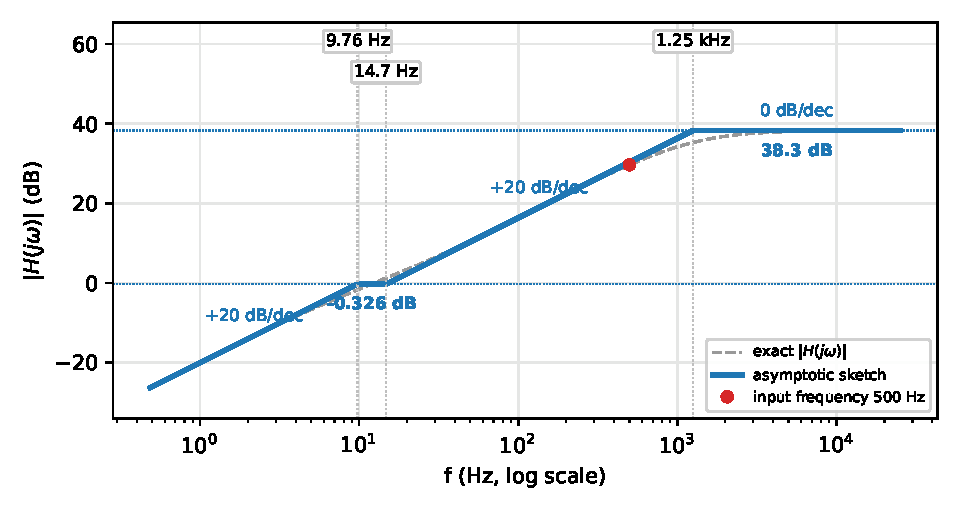
\includegraphics[width=0.78\linewidth,height=6.5cm,keepaspectratio]{p16_bode}\end{center}

{\small Blue: the straight-line sketch you are expected to draw. Dashed grey: the exact curve (about 3\,dB below the corner of an isolated pole). Red dot: the input frequency of Step 7.}
\solstep{7}{Steady-state output}The input is $V_i(t) = 0.01\sin\left(2\pi\cdot 500\,t\right)$, so $\omega_{in} = 2\pi\cdot 500 = 3140$\,rad/s. Put $s=j\omega_{in}$ in each factor (tool T5): magnitudes multiply, angles add.
{\small Rules: $\left|\frac{s}{s+p}\right| = \frac{\omega}{\sqrt{\omega^2+p^2}}$, $\angle = \frac{\pi}{2}-\tan^{-1}\frac{\omega}{p}$;\quad $\left|\frac{1}{1+s/p}\right| = \frac{1}{\sqrt{1+(\omega/p)^2}}$, $\angle = -\tan^{-1}\frac{\omega}{p}$;\quad $\left|1+\frac{s}{z}\right| = \sqrt{1+(\omega/z)^2}$, $\angle = \tan^{-1}\frac{\omega}{z}$;\quad a negative $K$ adds $-\pi$.}
\begin{center}\renewcommand{\arraystretch}{1.35}
\begin{tabular}{ccc}
\toprule
factor & magnitude & angle (rad) \\
\midrule
$-0.963$ & $0.9632$ & $-3.14$ \\
$\rule[-1.1em]{0pt}{2.8em}\dfrac{s}{s+2\pi\cdot 9.76}$ & $0.9998$ & $0.0195$ \\
$\rule[-1.1em]{0pt}{2.8em}\left(1+\dfrac{s}{2\pi\cdot 14.7}\right)$ & $33.98$ & $1.54$ \\
$\rule[-1.7em]{0pt}{4em}\dfrac{1}{1+\dfrac{s}{2\pi\cdot 1.25\mathrm{k}}}$ & $0.9288$ & $-0.38$ \\
\textbf{total} & $\mathbf{30.39}$ (product) & $\mathbf{-1.96}$ (sum) \\
\bottomrule
\end{tabular}\end{center}

\begin{align*}
|H(j\omega_{in})| &= 30.4, \qquad \angle H(j\omega_{in}) = -1.96\ \mathrm{rad} \\
v_{o,ac}(t) &= 30.4\times 0.01\,\sin\left(2\pi\cdot 500\,t - 1.96\right) = 0.304\,\sin\left(2\pi\cdot 500\,t - 1.96\right)
\end{align*}

\[
\boxed{V_o(t) = 0.304\,\sin\left(2\pi\cdot 500\,t - 1.96\right)\ \mathrm{V}}
\]

\begin{ansbox}
$H(s) = -0.963\,\dfrac{s}{s+2\pi\cdot 9.76}\,\left(1+\dfrac{s}{2\pi\cdot 14.7}\right)\,\dfrac{1}{1+\dfrac{s}{2\pi\cdot 1.25\mathrm{k}}}$\quad (corners: 9.76 Hz, 14.7 Hz, 1.25 kHz)\\[4pt]
$V_o(t) = 0.304\,\sin\left(2\pi\cdot 500\,t - 1.96\right)\ \mathrm{V}$
\end{ansbox}

\newpage
\subsection*{Solution 4D.17 \hfill Hard}
\begin{center}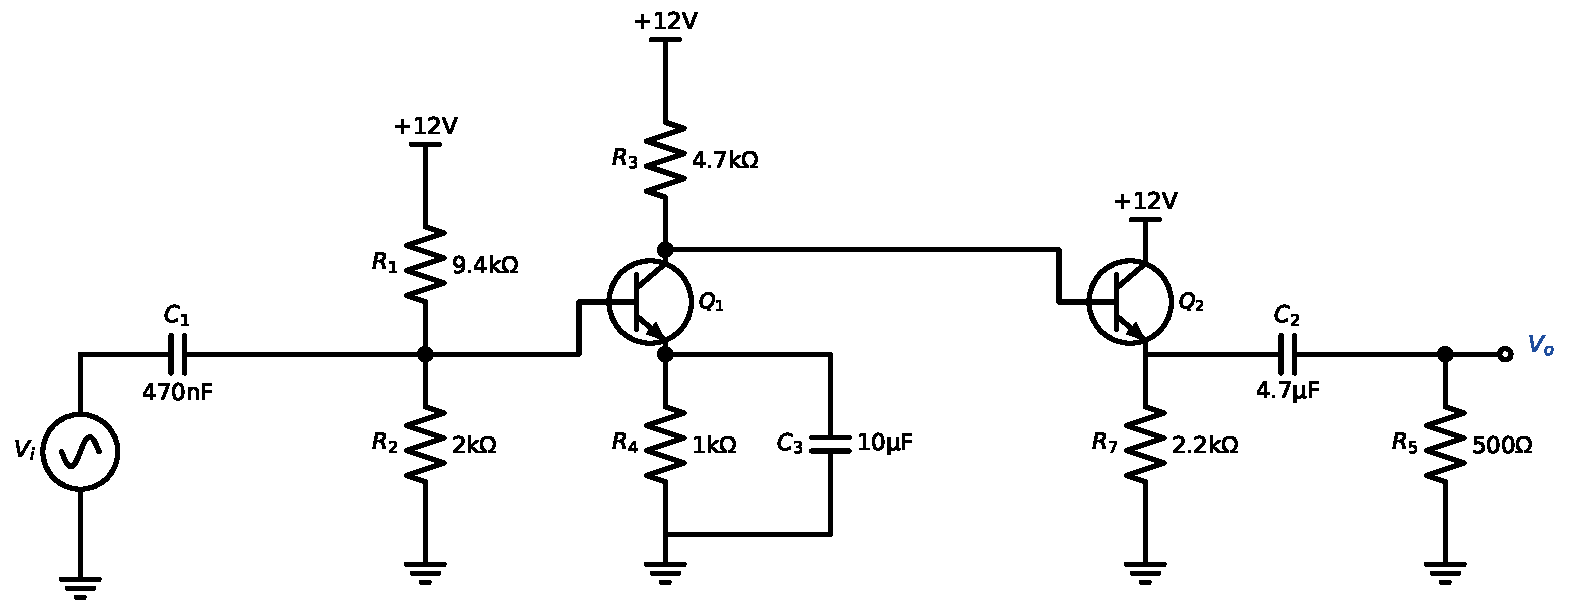
\includegraphics[width=0.9\linewidth,height=6cm,keepaspectratio]{p17_circuit}\end{center}
\solstep{1}{DC currents and small-signal parameters}The DC collector currents are given: $I_{C1} = 1.41\,\mathrm{m}\mathrm{A}$, $I_{C2} = 2.13\,\mathrm{m}\mathrm{A}$. For AC every DC supply is ground and every ``$\infty$'' capacitor is a short (tool T3). Small-signal emitter resistances (tool T3):\begin{align*}
r_{e1} &= \frac{V_T}{I_{C1}} = \frac{25\,\mathrm{mV}}{1.41\,\mathrm{m}\mathrm{A}} = 17.8\,\Omega \\
r_{e2} &= \frac{V_T}{I_{C2}} = \frac{25\,\mathrm{mV}}{2.13\,\mathrm{m}\mathrm{A}} = 11.7\,\Omega
\end{align*}

\solstep{2}{Input resistance of each stage}Input resistance of every stage, from the last stage back to the first (each one loads the stage before it; tool T4):\begin{align*}
R_{i1} &= Z_{base,1} = (\beta+1)(r_{e1} + R_{4} \parallel \frac{1}{sC_{3}}) = \dfrac{1800\,s + 1.03\times 10^{7}}{s + 100} \\
R_{i2} &= Z_{base,2} = (\beta+1)(r_{e2} + R_{7} \parallel \left(\frac{1}{sC_{2}} + R_{5}\right)) = \dfrac{42300\,s + 1.76\times 10^{7}}{s + 78.8}
\end{align*}

\solstep{3}{Gain along the signal path}Multiply the node-to-node gains along the signal path (tool T4):\[
H(s) = \frac{v_{b1}}{v_i}\cdot\frac{v_{c1}}{v_{b1}}\cdot\frac{v_{e2}}{v_{b2}}\cdot\frac{v_o}{v_{e2}}
\]
\begin{align*}
\frac{v_{b1}}{v_i} &= \frac{R_{1} \parallel R_{2} \parallel R_{i1}}{\frac{1}{sC_{1}} + R_{1} \parallel R_{2} \parallel R_{i1}} = \dfrac{s^{2} + 5720\,s}{s^{2} + 8200\,s + 7.5\times 10^{6}} \\
\frac{v_{c1}}{v_{b1}} &= -\alpha\frac{Z_{C1}}{r_{e1} + Z_{E1}},\quad Z_{C1} = R_{3} \parallel R_{i2},\ Z_{E1} = R_{4} \parallel \frac{1}{sC_{3}}\ \Rightarrow\ \dfrac{-235\,s^{2} - 1.21\times 10^{5}\,s - 9.79\times 10^{6}}{s^{2} + 6100\,s + 2.19\times 10^{6}} \\
\frac{v_{e2}}{v_{b2}} &= \frac{Z_{E2}}{r_{e2} + Z_{E2}},\quad Z_{E2} = R_{7} \parallel \left(\frac{1}{sC_{2}} + R_{5}\right)\ \Rightarrow\ \dfrac{0.972\,s + 414}{s + 416} \\
\frac{v_o}{v_{e2}} &= \frac{R_{5}}{\frac{1}{sC_{2}} + R_{5}} = \dfrac{s}{s + 426}
\end{align*}

\solstep{4}{Transfer function}Multiply and simplify:\[
H(s) = \dfrac{-229\,s^{3} - 22900\,s^{2}}{s^{3} + 8580\,s^{2} + 1.06\times 10^{7}\,s + 2.87\times 10^{9}}
\]

\solstep{5}{Standard (Bode-ready) form}Find the roots. Every root $s=-p$ of the denominator is a \emph{pole}, every root $s=-z$ of the numerator is a \emph{zero}; $|p|$ and $|z|$ are the corner frequencies (rad/s).
\begin{itemize}[leftmargin=*,itemsep=2pt]
\item Numerator: it has the factor $s^2$ $\Rightarrow$ 2 zeros at $s=0$.
\item Numerator (after taking out the $s$ factor): $-229\,s - 22900$; divide by the leading coefficient $-229$ (this does not move the roots): $s + 100$; $s + 100 = 0 \Rightarrow s = -100$.
\item Denominator: $s^{3} + 8580\,s^{2} + 1.06\times 10^{7}\,s + 2.87\times 10^{9}$; this is degree 3: use a calculator's polynomial solver (or \texttt{numpy.roots}) $\Rightarrow s = -382,\ -1050,\ -7150$.
\end{itemize}

Factored form (leading coefficient in front):
\[
H(s) = -229\,\dfrac{s^{2}(s+100)}{(s+382)(s+1050)(s+7150)}
\]

Bode-ready form: rewrite every $(s+p) = p\left(1+\frac{s}{p}\right)$ and $(s+z) = z\left(1+\frac{s}{z}\right)$, and collect all constants into $K$. Each $s$ in the numerator is paired with one of the \emph{lowest} poles as $\frac{s}{s+p}$ (that factor is $\approx 1$ above $p$). Then every factor except $K$ is $\approx 1$ inside the pass-band:
\[
H(s) = -3.2\,\dfrac{s}{s+2\pi\cdot 60.8}\,\dfrac{s}{s+2\pi\cdot 167}\,\left(1+\dfrac{s}{2\pi\cdot 15.9}\right)\,\dfrac{1}{1+\dfrac{s}{2\pi\cdot 1.14\mathrm{k}}},\qquad K = -3.2
\]

\begin{center}\renewcommand{\arraystretch}{1.35}
\begin{tabular}{cccc}
\toprule
type & $\omega_c$ (rad/s) & $f_c=\omega_c/2\pi$ & slope change \\
\midrule
zero & $100$ & 15.9 Hz & $+20$ dB/dec \\
pole & $382$ & 60.8 Hz & $-20$ dB/dec \\
pole & $1050$ & 167 Hz & $-20$ dB/dec \\
pole & $7150$ & 1.14 kHz & $-20$ dB/dec \\
\bottomrule
\end{tabular}\end{center}

\solstep{6}{Magnitude Bode plot}Below every corner $|H(s)|\approx 7.99\times 10^{-6}\,s^2$, so the plot starts with a slope of $+40$\,dB/dec. Then, moving right, each pole bends the line down by 20\,dB/dec and each zero bends it up by 20\,dB/dec (tool T6):
\begin{center}\renewcommand{\arraystretch}{1.35}
\begin{tabular}{lcl}
\toprule
frequency range & slope & asymptote level \\
\midrule
$f<$ 15.9 Hz & $+40$ dB/dec & -22 dB at end \\
15.9 Hz -- 60.8 Hz & $+60$ dB/dec & -22 dB at start, 13 dB at end \\
60.8 Hz -- 167 Hz & $+40$ dB/dec & 13 dB at start, 30.5 dB at end \\
167 Hz -- 1.14 kHz & $+20$ dB/dec & 30.5 dB at start, 47.2 dB at end \\
$f>$ 1.14 kHz & $0$ dB/dec (flat) & 47.2 dB at start \\
\bottomrule
\end{tabular}\end{center}

\begin{center}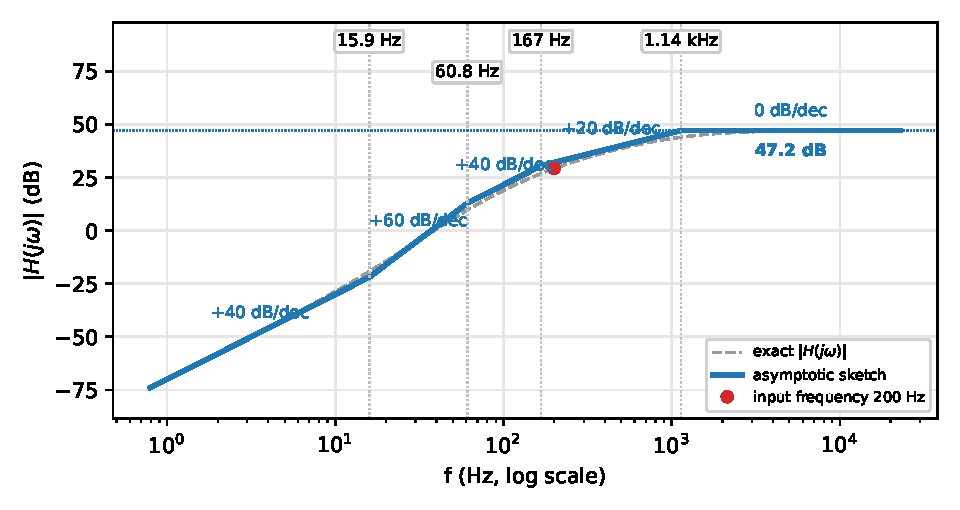
\includegraphics[width=0.78\linewidth,height=6.5cm,keepaspectratio]{p17_bode}\end{center}

{\small Blue: the straight-line sketch you are expected to draw. Dashed grey: the exact curve (about 3\,dB below the corner of an isolated pole). Red dot: the input frequency of Step 7.}
\solstep{7}{Steady-state output}The input is $V_i(t) = 0.002\cos\left(2\pi\cdot 200\,t-\frac{\pi}{3}\right)$, so $\omega_{in} = 2\pi\cdot 200 = 1260$\,rad/s. Put $s=j\omega_{in}$ in each factor (tool T5): magnitudes multiply, angles add.
{\small Rules: $\left|\frac{s}{s+p}\right| = \frac{\omega}{\sqrt{\omega^2+p^2}}$, $\angle = \frac{\pi}{2}-\tan^{-1}\frac{\omega}{p}$;\quad $\left|\frac{1}{1+s/p}\right| = \frac{1}{\sqrt{1+(\omega/p)^2}}$, $\angle = -\tan^{-1}\frac{\omega}{p}$;\quad $\left|1+\frac{s}{z}\right| = \sqrt{1+(\omega/z)^2}$, $\angle = \tan^{-1}\frac{\omega}{z}$;\quad a negative $K$ adds $-\pi$.}
\begin{center}\renewcommand{\arraystretch}{1.35}
\begin{tabular}{ccc}
\toprule
factor & magnitude & angle (rad) \\
\midrule
$-3.2$ & $3.203$ & $-3.14$ \\
$\rule[-1.1em]{0pt}{2.8em}\dfrac{s}{s+2\pi\cdot 60.8}$ & $0.9567$ & $0.295$ \\
$\rule[-1.1em]{0pt}{2.8em}\dfrac{s}{s+2\pi\cdot 167}$ & $0.7675$ & $0.696$ \\
$\rule[-1.1em]{0pt}{2.8em}\left(1+\dfrac{s}{2\pi\cdot 15.9}\right)$ & $12.61$ & $1.49$ \\
$\rule[-1.7em]{0pt}{4em}\dfrac{1}{1+\dfrac{s}{2\pi\cdot 1.14\mathrm{k}}}$ & $0.9849$ & $-0.174$ \\
\textbf{total} & $\mathbf{29.2}$ (product) & $\mathbf{-0.833}$ (sum) \\
\bottomrule
\end{tabular}\end{center}

\begin{align*}
|H(j\omega_{in})| &= 29.2, \qquad \angle H(j\omega_{in}) = -0.833\ \mathrm{rad} \\
v_{o,ac}(t) &= 29.2\times 0.002\,\cos\left(2\pi\cdot 200\,t - 1.88\right) = 0.0584\,\cos\left(2\pi\cdot 200\,t - 1.88\right)
\end{align*}

(phase: $\theta + \angle H = -\frac{\pi}{3} + (-0.833) = -1.88$\,rad.)
\[
\boxed{V_o(t) = 0.0584\,\cos\left(2\pi\cdot 200\,t - 1.88\right)\ \mathrm{V}}
\]

\begin{ansbox}
$H(s) = -3.2\,\dfrac{s}{s+2\pi\cdot 60.8}\,\dfrac{s}{s+2\pi\cdot 167}\,\left(1+\dfrac{s}{2\pi\cdot 15.9}\right)\,\dfrac{1}{1+\dfrac{s}{2\pi\cdot 1.14\mathrm{k}}}$\quad (corners: 15.9 Hz, 60.8 Hz, 167 Hz, 1.14 kHz)\\[4pt]
$V_o(t) = 0.0584\,\cos\left(2\pi\cdot 200\,t - 1.88\right)\ \mathrm{V}$
\end{ansbox}

\newpage
\subsection*{Solution 4D.18 \hfill Hard}
\begin{center}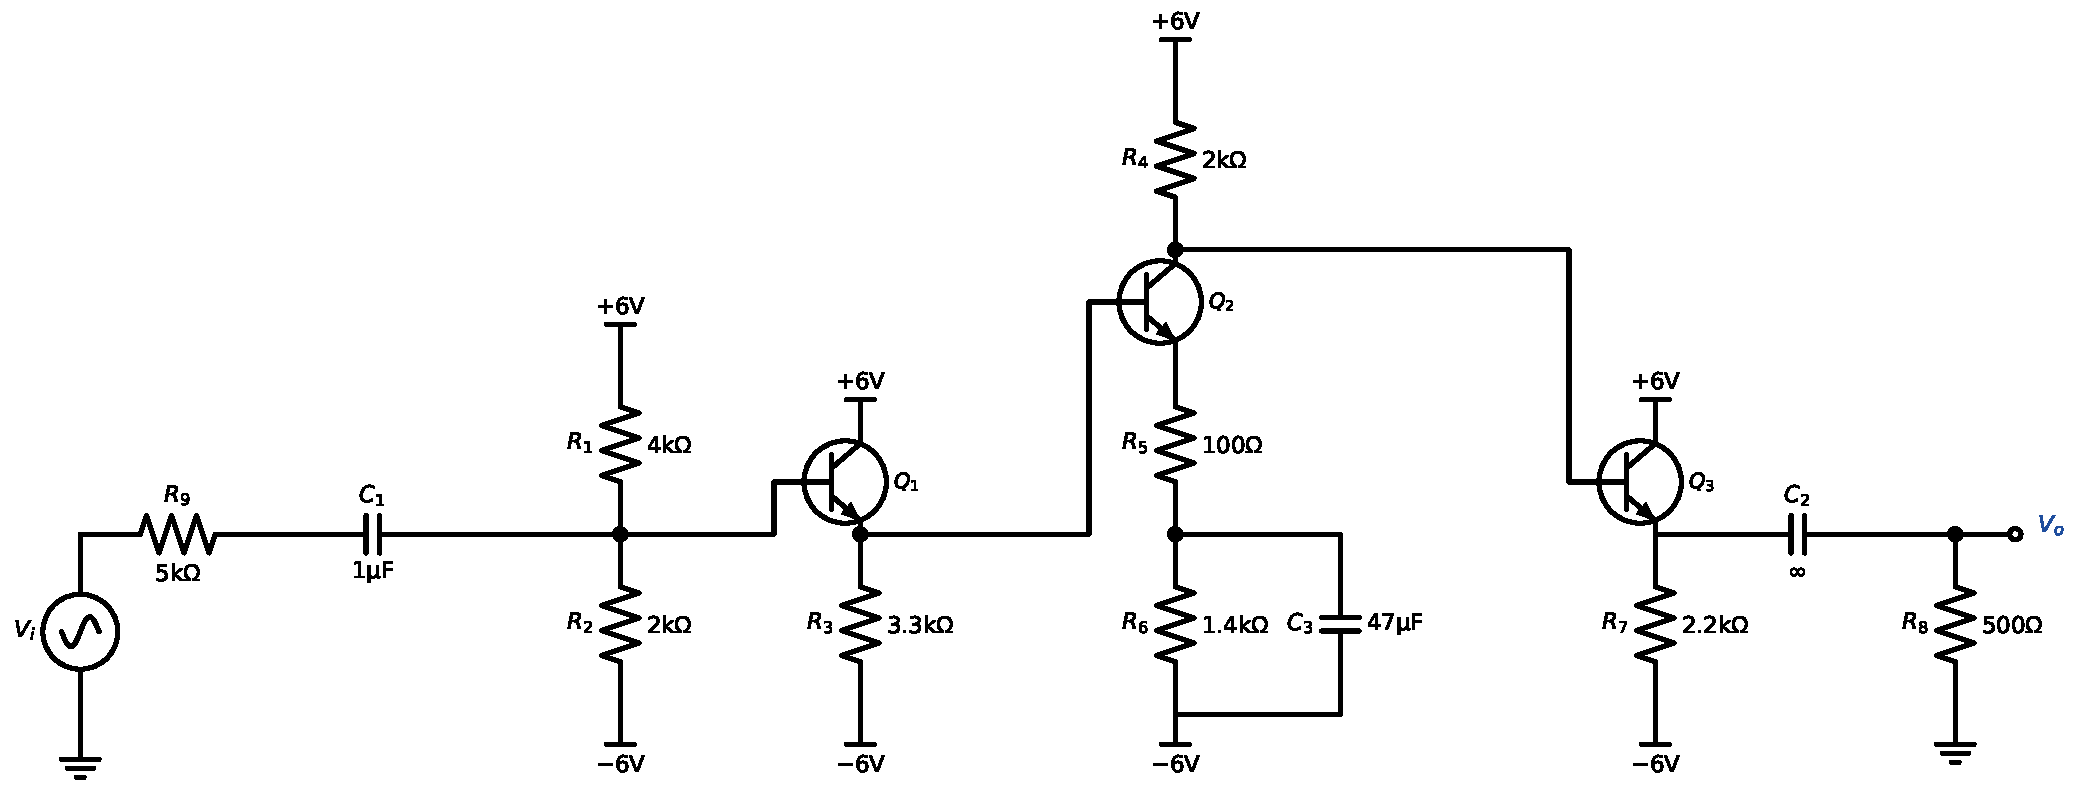
\includegraphics[width=0.9\linewidth,height=6cm,keepaspectratio]{p18_circuit}\end{center}
\solstep{1}{DC currents and small-signal parameters}The DC collector currents are given: $I_{C1} = 1\,\mathrm{m}\mathrm{A}$, $I_{C2} = 1.73\,\mathrm{m}\mathrm{A}$, $I_{C3} = 3.56\,\mathrm{m}\mathrm{A}$. For AC every DC supply is ground and every ``$\infty$'' capacitor is a short (tool T3). Small-signal emitter resistances (tool T3):\begin{align*}
r_{e1} &= \frac{V_T}{I_{C1}} = \frac{25\,\mathrm{mV}}{1\,\mathrm{m}\mathrm{A}} = 25\,\Omega \\
r_{e2} &= \frac{V_T}{I_{C2}} = \frac{25\,\mathrm{mV}}{1.73\,\mathrm{m}\mathrm{A}} = 14.4\,\Omega \\
r_{e3} &= \frac{V_T}{I_{C3}} = \frac{25\,\mathrm{mV}}{3.56\,\mathrm{m}\mathrm{A}} = 7.02\,\Omega
\end{align*}

\solstep{2}{Input resistance of each stage}Input resistance of every stage, from the last stage back to the first (each one loads the stage before it; tool T4):\begin{align*}
R_{i1} &= Z_{base,1} = (\beta+1)(r_{e1} + R_{3} \parallel R_{i2}) = \dfrac{2.62\times 10^{5}\,s + 5.26\times 10^{7}}{s + 160} \\
R_{i2} &= Z_{base,2} = (\beta+1)(r_{e2} + R_{5} + \left(R_{6} \parallel \frac{1}{sC_{3}}\right)) = \dfrac{11600\,s + 2.32\times 10^{6}}{s + 15.2} \\
R_{i3} &= Z_{base,3} = (\beta+1)(r_{e3} + R_{7} \parallel R_{8}) = 41.9\,\mathrm{k}\Omega
\end{align*}

\solstep{3}{Gain along the signal path}Multiply the node-to-node gains along the signal path (tool T4):\[
H(s) = \frac{v_{b1}}{v_i}\cdot\frac{v_{e1}}{v_{b1}}\cdot\frac{v_{c2}}{v_{b2}}\cdot\frac{v_{e3}}{v_{b3}}
\]
\begin{align*}
\frac{v_{b1}}{v_i} &= \frac{R_{1} \parallel R_{2} \parallel R_{i1}}{R_{9} + \frac{1}{sC_{1}} + R_{1} \parallel R_{2} \parallel R_{i1}} = \dfrac{0.21\,s^{2} + 42.1\,s}{s^{2} + 359\,s + 31700} \\
\frac{v_{e1}}{v_{b1}} &= \frac{Z_{E1}}{r_{e1} + Z_{E1}},\quad Z_{E1} = R_{3} \parallel R_{i2}\ \Rightarrow\ \dfrac{0.99\,s + 199}{s + 201} \\
\frac{v_{c2}}{v_{b2}} &= -\alpha\frac{Z_{C2}}{r_{e2} + Z_{E2}},\quad Z_{C2} = R_{4} \parallel R_{i3},\ Z_{E2} = R_{5} + \left(R_{6} \parallel \frac{1}{sC_{3}}\right)\ \Rightarrow\ \dfrac{-16.5\,s - 251}{s + 201} \\
\frac{v_{e3}}{v_{b3}} &= \frac{Z_{E3}}{r_{e3} + Z_{E3}},\quad Z_{E3} = R_{7} \parallel R_{8}\ \Rightarrow\ 0.983
\end{align*}

\solstep{4}{Transfer function}Multiply and simplify:\[
H(s) = \dfrac{-3.37\,s^{2} - 51.2\,s}{s^{2} + 359\,s + 31700}
\]

\solstep{5}{Standard (Bode-ready) form}Find the roots. Every root $s=-p$ of the denominator is a \emph{pole}, every root $s=-z$ of the numerator is a \emph{zero}; $|p|$ and $|z|$ are the corner frequencies (rad/s).
\begin{itemize}[leftmargin=*,itemsep=2pt]
\item Numerator: it has the factor $s$ $\Rightarrow$ 1 zero at $s=0$.
\item Numerator (after taking out the $s$ factor): $-3.37\,s - 51.2$; divide by the leading coefficient $-3.37$ (this does not move the roots): $s + 15.2$; $s + 15.2 = 0 \Rightarrow s = -15.2$.
\item Denominator: $s^{2} + 359\,s + 31700$; quadratic formula:\[
s = \frac{-359 \pm \sqrt{(359)^2 - 4(31700)}}{2} = \frac{-359 \pm 42.8}{2} \Rightarrow s = -158,\ -201
\]

\end{itemize}

Factored form (leading coefficient in front):
\[
H(s) = -3.37\,\dfrac{s(s+15.2)}{(s+158)(s+201)}
\]

Bode-ready form: rewrite every $(s+p) = p\left(1+\frac{s}{p}\right)$ and $(s+z) = z\left(1+\frac{s}{z}\right)$, and collect all constants into $K$. Each $s$ in the numerator is paired with one of the \emph{lowest} poles as $\frac{s}{s+p}$ (that factor is $\approx 1$ above $p$). Then every factor except $K$ is $\approx 1$ inside the pass-band:
\[
H(s) = -0.255\,\dfrac{s}{s+2\pi\cdot 25.1}\,\left(1+\dfrac{s}{2\pi\cdot 2.42}\right)\,\dfrac{1}{1+\dfrac{s}{2\pi\cdot 31.9}},\qquad K = -0.255
\]

\begin{center}\renewcommand{\arraystretch}{1.35}
\begin{tabular}{cccc}
\toprule
type & $\omega_c$ (rad/s) & $f_c=\omega_c/2\pi$ & slope change \\
\midrule
zero & $15.2$ & 2.42 Hz & $+20$ dB/dec \\
pole & $158$ & 25.1 Hz & $-20$ dB/dec \\
pole & $201$ & 31.9 Hz & $-20$ dB/dec \\
\bottomrule
\end{tabular}\end{center}

\solstep{6}{Magnitude Bode plot}Below every corner $|H(s)|\approx 0.00162\,s$, so the plot starts with a slope of $+20$\,dB/dec. Then, moving right, each pole bends the line down by 20\,dB/dec and each zero bends it up by 20\,dB/dec (tool T6):
\begin{center}\renewcommand{\arraystretch}{1.35}
\begin{tabular}{lcl}
\toprule
frequency range & slope & asymptote level \\
\midrule
$f<$ 2.42 Hz & $+20$ dB/dec & -32.2 dB at end \\
2.42 Hz -- 25.1 Hz & $+40$ dB/dec & -32.2 dB at start, 8.47 dB at end \\
25.1 Hz -- 31.9 Hz & $+20$ dB/dec & 8.47 dB at start, 10.6 dB at end \\
$f>$ 31.9 Hz & $0$ dB/dec (flat) & 10.6 dB at start \\
\bottomrule
\end{tabular}\end{center}

\begin{center}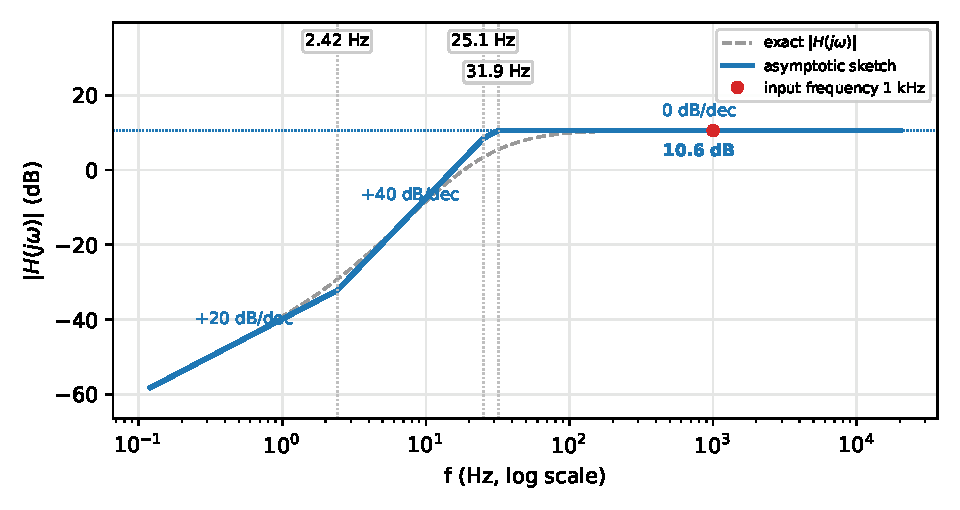
\includegraphics[width=0.78\linewidth,height=6.5cm,keepaspectratio]{p18_bode}\end{center}

{\small Blue: the straight-line sketch you are expected to draw. Dashed grey: the exact curve (about 3\,dB below the corner of an isolated pole). Red dot: the input frequency of Step 7.}
\solstep{7}{Steady-state output}The input is $V_i(t) = 0.01\sin\left(2\pi\cdot 1000\,t\right)$, so $\omega_{in} = 2\pi\cdot 1000 = 6280$\,rad/s. Put $s=j\omega_{in}$ in each factor (tool T5): magnitudes multiply, angles add.
{\small Rules: $\left|\frac{s}{s+p}\right| = \frac{\omega}{\sqrt{\omega^2+p^2}}$, $\angle = \frac{\pi}{2}-\tan^{-1}\frac{\omega}{p}$;\quad $\left|\frac{1}{1+s/p}\right| = \frac{1}{\sqrt{1+(\omega/p)^2}}$, $\angle = -\tan^{-1}\frac{\omega}{p}$;\quad $\left|1+\frac{s}{z}\right| = \sqrt{1+(\omega/z)^2}$, $\angle = \tan^{-1}\frac{\omega}{z}$;\quad a negative $K$ adds $-\pi$.}
\begin{center}\renewcommand{\arraystretch}{1.35}
\begin{tabular}{ccc}
\toprule
factor & magnitude & angle (rad) \\
\midrule
$-0.255$ & $0.2553$ & $-3.14$ \\
$\rule[-1.1em]{0pt}{2.8em}\dfrac{s}{s+2\pi\cdot 25.1}$ & $0.9997$ & $0.0251$ \\
$\rule[-1.1em]{0pt}{2.8em}\left(1+\dfrac{s}{2\pi\cdot 2.42}\right)$ & $413.4$ & $1.57$ \\
$\rule[-1.7em]{0pt}{4em}\dfrac{1}{1+\dfrac{s}{2\pi\cdot 31.9}}$ & $0.03193$ & $-1.54$ \\
\textbf{total} & $\mathbf{3.369}$ (product) & $\mathbf{-3.09}$ (sum) \\
\bottomrule
\end{tabular}\end{center}

\begin{align*}
|H(j\omega_{in})| &= 3.37, \qquad \angle H(j\omega_{in}) = -3.09\ \mathrm{rad} \\
v_{o,ac}(t) &= 3.37\times 0.01\,\sin\left(2\pi\cdot 1000\,t - 3.09\right) = 0.0337\,\sin\left(2\pi\cdot 1000\,t - 3.09\right)
\end{align*}

\[
\boxed{V_o(t) = 0.0337\,\sin\left(2\pi\cdot 1000\,t - 3.09\right)\ \mathrm{V}}
\]

\begin{ansbox}
$H(s) = -0.255\,\dfrac{s}{s+2\pi\cdot 25.1}\,\left(1+\dfrac{s}{2\pi\cdot 2.42}\right)\,\dfrac{1}{1+\dfrac{s}{2\pi\cdot 31.9}}$\quad (corners: 2.42 Hz, 25.1 Hz, 31.9 Hz)\\[4pt]
$V_o(t) = 0.0337\,\sin\left(2\pi\cdot 1000\,t - 3.09\right)\ \mathrm{V}$
\end{ansbox}

\end{document}
